\documentclass[12pt]{report}
\usepackage{array, amssymb, amsthm, linguex, enumerate, amsmath, physics, enumitem, xcolor, graphicx, xparse}
\let\fg\undefined %remove linguex/siunitx naming clash
\usepackage[english]{babel}
\usepackage[letterpaper,top=2cm,bottom=2cm,left=3cm,right=3cm,marginparwidth=1.75cm]{geometry}
\usepackage[colorlinks=true, allcolors=blue]{hyperref}
\usepackage[group-separator={,}]{siunitx} %\num{12345} -> "12,345"
\usepackage{listings} %code listings
\graphicspath{{images/}}

%Number sets
\newcommand{\R}{\mathbb{R}}
\newcommand{\C}{\mathbb{C}}
\newcommand{\N}{\mathbb{N}}
\newcommand{\F}{\mathbb{F}}
\renewcommand{\Re}{\operatorname{Re}}
\renewcommand{\Im}{\operatorname{Im}}
\renewcommand{\L}[1]{\mathcal{L}\left({#1}\right)} %Linear Map

\newcommand{\pmp}{\,\pm\,} %add small extra space to \pm

\NewDocumentCommand{\ceil}{ s m }{% ceiling brackets
    \IfBooleanTF{#1}%
    {\lceil #2 \rceil}% starred: no-autosizing
    {\left\lceil #2 \right\rceil}% unstarred: autosizing
}

\NewDocumentCommand{\ceiling}{ s m }{% ceiling brackets
    \IfBooleanTF{#1}%
    {\lceil #2 \rceil}% starred: no-autosizing
    {\left\lceil #2 \right\rceil}% unstarred: autosizing
}

\NewDocumentCommand{\floor}{ s m }{% floor brackets
    \IfBooleanTF{#1}%
    {\lfloor #2 \rfloor}% starred: no-autosizing
    {\left\lfloor #2 \right\rfloor}% unstarred: autosizing
}

\NewDocumentCommand{\pars}{ s m }{% parenthesis
    \IfBooleanTF{#1}%
    {( #2 ) }% starred: no-autosizing
    {\left( #2 \right) }% unstarred: autosizing
}

\NewDocumentCommand{\inner}{ s m }{% inner product
    \IfBooleanTF{#1}%
    {\langle #2 \rangle}% starred: no-autosizing
    {\left\langle #2 \right\rangle}% unstarred: autosizing
}

\NewDocumentCommand{\brac}{ s m }{% brackets
    \IfBooleanTF{#1}%
    {[#2] }% starred: no-autosizing
    {\left[ #2 \right] }% unstarred: autosizing
}

%default latex bracket size naming
\newcommand{\biggbrac}[1]{\bigg[ {#1} \bigg] }
\newcommand{\bigbrac}[1]{\big[ {#1} \big] }
\newcommand{\Bigbrac}[1]{\Big[ {#1} \Big] }


\RenewDocumentCommand{\over}{ s m }{% fraction 1/arg
    \IfBooleanTF{#1}%
    {\dfrac{1}{#2}}% starred: dfrac
    {\frac{1}{#2}}% unstarred: normal frac
}

\NewDocumentCommand{\pover}{ s m }{% parenthesis around fraction (1/arg)
    \IfBooleanTF{#1}%
    {\left(\dfrac{1}{#2}\right)}% starred: dfrac
    {\left(\frac{1}{#2}\right)}% unstarred: normal frac
}

\NewDocumentCommand{\pfrac}{ s m m}{% parenthesis around fraction (arg1/arg2)
    \IfBooleanTF{#1}%
    {\left( \dfrac{{#2}}{{#3}} \right)}% starred: dfrac
    {\left( \frac{{#2}}{{#3}} \right)}% unstarred: normal frac
}


\newcommand{\Xbar}{\bar{X}}
\newcommand{\Ybar}{\bar{Y}}
\newcommand{\xbar}{\bar{x}}
\newcommand{\ybar}{\bar{y}}


\newcommand{\limn}{\lim_{n\to\infty}}

\newcommand{\gammaDist}[2]{\operatorname{Gamma} \left( {#1},{#2} \right)} %gamma distribution
\NewDocumentCommand{\normalDist}{s g g}{ %normal distibution
    \IfBooleanTF{#1} { % starred, no autosizing parenthesis
      \IfNoValueTF{#2}{
          N (\mu,\, \sigma^2 ) %\normalDist* "default" normal distribution N(\mu, \sigma^2)
        } {
            \IfNoValueTF{#3}{N (#2)}{} %\normalDist{arg} --> N(arg)
        }
      \IfNoValueTF{#3}{}{N ( #2, #3 )}  %\normalDist*{arg1}{arg2} --> N(arg1,arg2)
    }  % else (unstarred) autosize parenthesis
    {
        \IfNoValueTF{#2}{
            N \left(\mu,\, \sigma^2 \right) %\normalDist "default" normal distribution N(\mu, \sigma^2)
        } {
            \IfNoValueTF{#3}{N \left(#2\right)}{} %\normalDist{arg} --> N(arg)
        }
        \IfNoValueTF{#3}{}{N \left( #2, #3 \right)} %\normalDist{arg1}{arg2} --> N(arg1,arg2)
    }
}



%colors
\definecolor{ggreen}{RGB}{0, 127, 0}
\definecolor{dgray}{RGB}{63,63,63}
\definecolor{neonorange}{RGB}{255,47,0}
\definecolor{mygray}{rgb}{0.5,0.5,0.5}
\definecolor{eblue}{RGB}{0,74,127}
\definecolor{darkorange}{RGB}{225,100,0}
\definecolor{gold}{RGB}{255,155,0}
\definecolor{purp}{RGB}{178,0,255}
\definecolor{turquoise}{RGB}{0,160,100}
\definecolor{brightblue}{RGB}{0,100,255}
\definecolor{mediumblue}{RGB}{0,125,200}
\newcommand{\red}[1]{\color{red}{#1}\color{black}}
\newcommand{\green}[1]{\color{ggreen}{#1}\color{black}}
\newcommand{\blue}[1]{\color{blue}{#1}\color{black}}
\newcommand{\setRed}{\color{red}}
\newcommand{\setBlack}{\color{black}}
\newcommand{\setBlue}{\color{blue}}
\newcommand{\setGreen}{\color{ggreen}}



\newcommand{\thru}[1]{{#1}_1, \dots, {#1}_n}
\newcommand{\sumThru}[1]{{#1}_1 + \cdots + {#1}_n}
\newcommand{\yn}{Y_1, \dots, Y_n} % Y_1, ..., Y_n
\newcommand{\xn}{X_1, \dots, X_n} % Y_1, ..., Y_n

%hats and tildes
\newcommand{\that}{\widehat{\theta}} % theta hat
\newcommand{\phat}{\widehat{p}} % p hat
\newcommand{\qhat}{\widehat{q}} % p hat
\newcommand{\psihat}{\widehat{\psi}} % psi hat
\newcommand{\Psihat}{\widehat{\Psi}} % Psi hat
\newcommand{\ptilde}{\widetilde{p}} % psi tilde
\newcommand{\Psitil}{\widetilde{\Psi}} % Psi tilde
\newcommand{\betah}{\widehat{\beta}} % beta hat
\newcommand{\muh}{\widehat{\mu}} % mu hat

\newcommand{\SSA}{\operatorname{SSA}} % sum square among
\newcommand{\SSW}{\operatorname{SSW}} % sum square within
\newcommand{\SST}{\operatorname{SST}} % sum square total

%2x2 matrix shortcuts
\newcommand{\detx}[4]{\begin{vmatrix}{#1} & {#2}\\{#3}&{#4}\end{vmatrix}} % 2x2 determinant
\newcommand{\bmat}[4]{\begin{bmatrix}{#1} & {#2}\\{#3}&{#4}\end{bmatrix}} % 2x2 matrix brackets
\renewcommand{\pmat}[4]{\begin{pmatrix}{#1} & {#2}\\{#3}&{#4}\end{pmatrix}} % 2x2 matrix parenthesis

%remove any enumerate/itemize indent temporarily
\makeatletter   %% <- make @ usable in macro names
\newcommand*\notab[1]{%
  \begingroup   %% <- limit scope of the following changes
    \par        %% <- start a new paragraph
    \@totalleftmargin=0pt \linewidth=\columnwidth
    %% ^^ let other commands know that the margins have been reset
    \parshape 0
    %% ^^ reset the margins
    #1\par      %% <- insert #1 and end this paragraph
  \endgroup
}
\makeatother    %% <- revert @


\newcommand{\dimrange}[1]{\operatorname{dim}\operatorname{range}{#1}} % dimrange
\newcommand{\dimnull}[1]{\operatorname{dim}\operatorname{null}{#1}} % dimnull
\newcommand{\range}[1]{\operatorname{range}{#1}} %range
\newcommand{\nullspace}{\operatorname{null}} %null

% polynomial notation
\NewDocumentCommand{\poly}{ s g g }{%
    \IfBooleanTF{#1} {
        \IfNoValueTF{#2} {
            \mathcal{P}(\mathbb{R})
        } {
            \mathcal{P}_{#2}(\mathbb{R})
        }
    } {
        \IfNoValueTF{#3} {
            {\mathcal{P}(#2)}
        } { %else
            {\mathcal{P}_{#2}(#3)}
        }
    }
}

\NewDocumentCommand{\bias}{ s m }{% bias(arg)
    \IfBooleanTF{#1}%
    {\operatorname{bias}(#2)}% starred: no autosizing
    {\operatorname{bias}\left(#2\right)}% unstarred: autosizing
}

\NewDocumentCommand{\MSE}{ s m }{% MSE(arg)
    \IfBooleanTF{#1}%
    {\operatorname{MSE}(#2)}% starred: no autosizing
    {\operatorname{MSE}\left(#2\right)}% unstarred: autosizing
}

\NewDocumentCommand{\Var}{ s m }{% variance with parenthesis V(arg)
    \IfBooleanTF{#1}%
    {\operatorname{Var}(#2)}% starred: no autosizing
    {\operatorname{Var}\left(#2\right)}% unstarred: autosizing
}

\NewDocumentCommand{\Varb}{ s m }{% variance with brackets V[arg]
    \IfBooleanTF{#1}%
    {\operatorname{Var}[\,#2\,]}% starred: no autosizing
    {\operatorname{Var}\left[\,#2\,\right]}% unstarred: has autosizing
}

\NewDocumentCommand{\Vb}{ s m }{% another renaming of variance with brackets V[arg]
    \IfBooleanTF{#1}%
    {\operatorname{Var}[\,#2\,]}% starred: no autosizing
    {\operatorname{Var}\left[\,#2\,\right]}% unstarred: has autosizing
}

\NewDocumentCommand{\E}{ s m }{% expectation with parenthesis E(arg)
    \IfBooleanTF{#1}%
    {\operatorname{E}(#2)}% starred: no autosizing
    {\operatorname{E}\left(#2\right)}% unstarred: has autosizing
}

\NewDocumentCommand{\Eb}{ s m }{% expectation with brackets E[arg]
    \IfBooleanTF{#1}%
    {\operatorname{E}[#2]}% starred: no autosizing
    {\operatorname{E}\left[#2\right]}% unstarred: has autosizing
}

\RenewDocumentCommand{\P}{ s m }{% probability with parenthesis Pr(arg)
    \IfBooleanTF{#1}%
    {\Pr (#2) }% starred: no autosizing
    {\Pr \left( #2 \right) }% unstarred: has autosizing
}

\NewDocumentCommand{\prob}{ s m }{% probability with parenthesis Pr(arg)
    \IfBooleanTF{#1}%
    {\Pr (#2) }% starred: no autosizing
    {\Pr \left( #2 \right) }% unstarred: has autosizing
}

\NewDocumentCommand{\eff}{ s m }{% efficiency with parenthesis eff(arg)
    \IfBooleanTF{#1}%
    {\operatorname{eff}(#2)}% starred: no autosizing
    {\operatorname{eff}\left(#2\right)}% unstarred: has autosizing
}

%vertical vector of up to 8 elements
\NewDocumentCommand\vvec{s m g g g g g g g}{%
    \IfBooleanTF{#1} {
        \begin{bmatrix}% if starred use brackets
            \IfNoValueTF{#2}{}{#2}
            \IfNoValueTF{#3}{}{\\#3}
            \IfNoValueTF{#4}{}{\\#4}
            \IfNoValueTF{#5}{}{\\#5}
            \IfNoValueTF{#6}{}{\\#6}
            \IfNoValueTF{#7}{}{\\#7}
            \IfNoValueTF{#8}{}{\\#8}
        \end{bmatrix}
    }  % else (unstarred) use parethesis
    {
        \begin{pmatrix}%
            \IfNoValueTF{#2}{}{#2}
            \IfNoValueTF{#3}{}{\\#3}
            \IfNoValueTF{#4}{}{\\#4}
            \IfNoValueTF{#5}{}{\\#5}
            \IfNoValueTF{#6}{}{\\#6}
            \IfNoValueTF{#7}{}{\\#7}
            \IfNoValueTF{#8}{}{\\#8}
        \end{pmatrix}
    }
}
\def\Cov{\operatorname{Cov}} %Covariance
\def\df{\text{df}} %degrees of freedom

\NewDocumentCommand{\example}{ s g }{% Example header
    \IfBooleanTF{#1}%
    {\vspace{0.1in}}% starred: 0.1in
    {\vspace{0.2in}}% unstarred: 0.2in
    \IfNoValueTF{#2} {\noindent\textbf{\color{eblue} Example: }}{\noindent\textbf{\color{eblue} Example (#2): }}
}
\NewDocumentCommand{\disc}{ s }{% Discussion header
    \IfBooleanTF{#1}%
    {\vspace{0.1in}\noindent\textbf{Discussion: } }% starred: 0.1in
    {\vspace{0.2in}\noindent\textbf{Discussion: } }% unstarred: 0.2in
}
\NewDocumentCommand{\defn}{ s }{% Definition header
    \IfBooleanTF{#1}%
    {\vspace{0.1in}\noindent\textbf{\color{neonorange} Definition: } }% starred: 0.1in
    {\vspace{0.2in}\noindent\textbf{\color{neonorange} Definition: } }% unstarred: 0.2in
}
\NewDocumentCommand{\reason}{ s }{% Reason header
    \IfBooleanTF{#1}%
    {\vspace{0.1in}\noindent\textbf{Reason:} }% starred: 0.1in
    {\vspace{0.2in}\noindent\textbf{Reason:} }% unstarred: 0.2in
}
\NewDocumentCommand{\recall}{ s }{% Recall header
    \IfBooleanTF{#1}%
    {\vspace{0.1in}\noindent\textit{Recall:} }% starred: 0.1in
    {\vspace{0.2in}\noindent\textit{Recall:} }% unstarred: 0.2in
}
\NewDocumentCommand{\remark}{ s }{% Remark header
    \IfBooleanTF{#1}%
    {\vspace{0.1in}\noindent\textit{Remark:} }% starred: 0.1in
    {\vspace{0.2in}\noindent\textit{Remark:} }% unstarred: 0.2in
}

\newcommand{\proj}[2]{\operatorname{proj}_{{#1}}{#2}} %projection
\newcommand{\wideand}{\qquad \text{and} \qquad}
\newcommand{\wideor}{\qquad \text{or} \qquad}

\newcommand{\bu}[1]{\textbf{\underline{{#1}}} } %bold underline
\newcommand{\boldit}[1]{\textbf{\textit{{#1}}} } %bold italix

% put actual quotation marks "around something"
\newcommand{\say}[1]{\textquotedblleft{#1}\textquotedblright}

% max{arg} and min{arg}
\renewcommand{\max}[1]{\operatorname{max}\left\{ #1 \right\}}
\renewcommand{\min}[1]{\operatorname{min}\left\{ #1 \right\}}

%circle around argument
\newcommand{\cir}[1]{\textcircled{\raisebox{-1pt}{#1}}}

% Updates the current chapter number.
% 0 based indices
\newcommand{\setChapter}[1]{
    \setcounter{chapter}{#1}
    \setcounter{section}{0}
}



% Update global section number, O based indices
\newcommand{\setSection}[1]{\setcounter{section}{#1}}



%Set table of contents depth
\setcounter{tocdepth}{3}


%Create a new vspace line no indent
\newcommand{\nl}{\vspace{0.1in}\noindent}
\newcommand{\nnl}{\vspace{0.2in}\noindent}
\newcommand{\nnnl}{\vspace{0.3in}\noindent}

% Code snippets
\newcommand{\code}[1]{{\fontfamily{qcr}\selectfont #1}}

\lstset{
    backgroundcolor=\color{white},
    basicstyle=\fontfamily{qcr}\footnotesize,
    breakatwhitespace=false,         % sets if automatic breaks should only happen at whitespace
    breaklines=true,                 % sets automatic line breaking
    captionpos=b,                    % sets the caption-position to bottom
    commentstyle=\color{dgray},    % comment style
    deletekeywords={...},            % if you want to delete keywords from the given language
    escapeinside={(*@}{@*)},          % if you want to add LaTeX within your code
    extendedchars=true,              % lets you use non-ASCII characters; for 8-bits encodings only, does not work with UTF-8
    firstnumber=1,                % start line enumeration with line 1
    frame=single,	                   % adds a frame around the code
    keepspaces=true,                 % keeps spaces in text, useful for keeping indentation of code (possibly needs columns=flexible)
    keywordstyle=\color{ggreen}\bfseries,       % keyword style
    language=SQL,                 % the language of the code
    morekeywords={*,...},            % if you want to add more keywords to the set
    numbers=left,                    % where to put the line-numbers; possible values are (none, left, right)
    numbersep=5pt,                   % how far the line-numbers are from the code
    numberstyle=\tiny\color{mygray}, % the style that is used for the line-numbers
    rulecolor=\color{black},         % if not set, the frame-color may be changed on line-breaks within not-black text (e.g. comments (green here))
    showspaces=false,                % show spaces everywhere adding particular underscores; it overrides 'showstringspaces'
    showstringspaces=false,          % underline spaces within strings only
    showtabs=false,                  % show tabs within strings adding particular underscores
    stringstyle=\bfseries\color{darkorange},     % string literal style
    tabsize=4	                   % sets default tabsize to 4 spaces
}

\lstdefinestyle{cpp}{language=C++,
    morekeywords={cout, cin, Comparable, T},numbers=none
}

\lstdefinestyle{sql}{
    language=sql,
    numbers=none,
    commentstyle=\color{ggreen},
    frame=none,
    keywords=[1]{SET, LEFT, OUTER, SELECT, UPDATE, DELETE, INSERT, INTO, FROM, GROUP, BY, INNER, JOIN, WHERE, DISTINCT, VALUES},
    keywordstyle=\bfseries,
    keywordstyle=[1]\color{eblue}\bfseries,
    keywords=[2]{AS, ON, NOT, AND, OR, IN, IS, NULL},
    keywordstyle=[2]\color{brightblue}\bfseries,
    keywords=[3]{COUNT, MAX, SUM, MIN},
    keywordstyle=[3]\color{purp}\bfseries,
    keywords=[4]{Eats, Person, Serves, Frequents, EMPLOYEE, WORKS\_ON, DEPENDENT, DEPT\_LOCATIONS, DEPARTMENT, PROJECT},
    keywordstyle=[4]\color{purp},
    keywords=[5]{name, age, gender, pizzeria, pizza, price, Fname, Lname, Ssn, Dno, Essn, Relationship, Dname, Dnumber, Mgr\_ssn, Mgr\_start\_date, Dlocation, Pno, Hours, Pname, Pnumber, Plocation, Dnum, Minit, Bdate, Address, Sex, Salary, Super\_ssn, Dependent\_name},
    keywordstyle=[5]\color{mediumblue}
}

%Remove hyphens
\tolerance=1
\emergencystretch=\maxdimen
\hyphenpenalty=10000
\hbadness=10000

%Page dimensions
\textwidth=6.5in
\hoffset=-0.25in
\textheight=9.5in
\voffset=0in

\begin{document}

\noindent
\begin{center}
    {\Huge \textbf{MATH 326}}
\end{center}
\begin{center}
    {\Large Probability \& Statistics II}\\[0.2cm]
    {\Large Tom Carty -- Spring 2022}\\[0.2cm]
    {\Large TeX'ed by Matthew Wilder (BU `23)}
\end{center}

\tableofcontents
\setChapter{-1}
\section*{Common Abbreviations and Notations}
\addcontentsline{toc}{section}{Abbreviations and Notations}
\begin{align*}
    \text{dist'n} &= \text{Distribution}\\
    \text{r.v.} &= \text{Random variable}\\
    \text{DOF} &= \text{degrees of freedom} \\
    \text{d.f.} &= \text{degrees of freedom} \\
    \text{MGF} &= \text{moment generating function} \\
    \text{mgf} &= \text{moment generating function}\\
    \text{pdf} &= \text{probability distribution function}\\
    \text{CLT} &= \text{Central Limit Theorem}\\
    \text{iid} &= \text{Independent Identically Distributed}\\
    \text{MSE} &= \text{Mean Square Error}\\
    \text{MoM} &= \text{Method of Moments}\\
    \text{MVUE} &= \text{Minimum Variance Unbiased Estimator}\\
    \text{MLE} &= \text{Maximum Likelihood Estimator}\\
    \mu &= \text{mean (average)}\\
    \sigma &= \text{standard deviation}\\
    \sigma^2 &= \text{variance}\\
    \Xbar &= \text{Sample mean}\\
    S &= \text{Sample standard deviation}\\
    S^2 &= \text{Sample variance}\\
    N(\mu,\sigma^2) &= \text{Normal distribution with: mean} = \mu \text{, variance} = \sigma^2\\
    Z &= \text{Z-score}
\end{align*}
\setChapter{6}
\chapter{Sampling Distributions and the Central Limit Theorem}
\section*{Chapter 7 Review}

Our first goal in Math 326 is to learn how to estimate global parameters of \say{population} like $\mu$ and $\sigma$. To do this, we need to understand how the random variable we use to estimate them are distributed. For example:
$$
\text{Parameters }\left\{\begin{aligned}
    \mu
    \\
    \sigma^2
\end{aligned}\right.
\hspace{0.5in}\text{Statistics }
\left\{\begin{aligned}
    \Xbar &= \over{n} \sum X_i
    \\
    S^2 &= \over{n-1} \sum \pars{X_i - \Xbar}^2
\end{aligned}\right.
$$

\setSection{1}
\section{Sample Means}

\begin{enumerate}[label=\textcircled{\raisebox{-1pt}{\arabic*}}]
    \item \textbf{Sample means: }
    \addcontentsline{toc}{subsection}{Theorem 7.1}

    \nl\textbf{Theorem 7.1}: Let $\yn$ be a random sample from $\normalDist*$ then $\Ybar$ is distributed by $\normalDist{\mu}{\dfrac{\sigma^2}{n}}$. The distribution of sample means, $\Ybar$, is also Normal.

    \reason* Linearity of Expectation and Variance properties 

    \disc* Recall in working with $\normalDist*$, we learned it was easier to standardize\\everything via
        $Z$-scores: $$Z = \frac{x-\mu}{\sigma}$$
        and $Z$ is distributed $\normalDist{0}{1}$, the \textbf{Standard Normal Distribution.}
        
        
    \item
        \textbf{Sample variance:}
        
        \nl Recall standard deviation $\sigma$ is a measure of the spread of the random variable and it's derived from $\pars{Y_i - \Ybar}^2$ terms. In all math, we normalize to take the \say{units} out of things.
        $$\underbrace{U_i = \frac{Y_i - \bar{Y}}{S}}_{\text{Data Driven = Stat}} \approx \underbrace{\frac{Y_i - \mu}{\sigma} = Z_i}_{\text{Not a stat}}$$
        
        \reason* $Z_i$ depends on unknown population parameters, nonetheless, it makes it easier to pretend that we start here.

        \addcontentsline{toc}{subsection}{Theorem 7.2}
        \nnl
        \textbf{Theorem 7.2} If $\yn$ are a random sample of $\normalDist*$. Then,
        $$U = \sum Z_i^2 = \sum \pars{\frac{Y_i - \mu}{\sigma}}^2$$
        has a $\chi^2$ distribution with $n$ degrees of freedom (df).

        \nl
        \textit{Recall}: $\chi^2$ distribution is a $\gammaDist{\dfrac{\nu}{2}}{2}$ where $\nu = \df$ (degrees of freedom).

        \reason In old homework (325), ${Z_i}^2$ is $\chi^2$ with $\df = 1$.
        By product of mgf, $\sum {Z_i}^2$ is $\chi^2$ with $\df = n$. Now to get sample variance, we do some algebra:
        \notab{\begin{align*}
            && S^2 &= \frac{1}{n-1}\sum(Y_i-\bar{Y})^2 \\
            &&& \approx \frac{1}{n-1}\sum(Y_i - \mu)^2 \\
            \iff && \frac{S^2}{\sigma^2} &\approx \frac{1}{n-1}\sum \pars{\frac{Y_i - \mu}{\sigma}}^2\\
            \iff && \frac{S^2(n-1)}{\sigma^2} &\approx \sum {Z_i}^2
        \end{align*}}

        \nl Showing it is okay to replace $\Ybar$ with $\mu$ is the point of the proof of the following theorem:

        \addcontentsline{toc}{subsection}{Theorem 7.3 (Fisher's Theorem)}
        
        \nnl \textbf{Theorem 7.3 (Fisher's Theorem)} The distribution of sample variance $S^2$

        \nl If $\yn$ is a random sample from $\normalDist*$. Then,
        \begin{enumerate}[label=\textcircled{\raisebox{-1pt}{\arabic*}}]
            \item 
                $\dfrac{S^2(n-1)}{\sigma^2}$ has $\chi^2$ distribution with $(n-1)$ degrees of freedom.
            
            \item
                $\bar{Y}$ and $S^2$ are independent random variables.

        \end{enumerate}

                    
        \item
        $t$-distribution and $F$-distribution
        $$\underbrace{\frac{Y_i-\mu}{\sigma}}_{\text{Normal}} \approx \underbrace{\frac{Y_i -\mu}{S}}_{\text{t-dist'n}} \approx \underbrace{\frac{Y_i - \bar{Y}}{S}}_{\text{Statistic}}$$

        \nl Address when to use what is the point of this class

        \nl Skip definitions (such as moments) for the time being

        \nl Also, The Law of Large Numbers. Used to prove the Central Limit Theorem.
\end{enumerate}








\newpage
\setSection{3}
\section{The Central Limit Theorem}

The reason Normal distributions play an outsized role in applied statistics is that the distribution of  $\bar{Y}$ can be made \emph{nearly normal}, no matter the underlying distribution of $Y$ (Does not need to start \say{life} Normal). So \emph{nearly} normal, that we just pretend it is.



\nnl \textbf{Theorem 7.4: The Central Limit Theorem (CLT)}

\nl Let $\yn$ be independent and identically distributed (iid) random variables with
$$\E{Y_i} = \mu \wideand \Var{Y_i} = \sigma^2 < \infty$$
(Need finite variance for CLT to hold)

\nl Define $$U_n = \frac{\bar{Y}-\mu}{\sqrt{\frac{\sigma^2}{n}}} = \frac{\sum (Y_i) - n\mu}{\sigma \sqrt{n}}.$$

\nl The CLT says the distribution function of
$U_n$ converges to $N(0,1)$ as $n\to\infty$.

\nl Big idea: The distribution $\Ybar$ can be thought of as $\normalDist{\mu}{\frac{\sigma^2}{n}}$.

\defn The \bu{support of $f$} is the domain on which $f$ is non-zero.

\example* Let $\Xbar$ denote the mean of a random sample of size $n=15$, from the distribution whose pdf is $$f(x) = \frac{3}{2}x^2, \qquad x \,\in\, [-1,1]$$


\nl Can be shown that
$$\mu = \Eb{X} = 0 \wideand \sigma^2 = \Eb{(X-\mu)^2} = \frac{3}{5}$$

\nl To compute $\P{0.03 \leq \Xbar \leq 0.15}$, we use the CLT and assume $\Xbar$ is distributed  by
$$\normalDist{\mu}{\frac{\sigma^2}{n}} = \normalDist{0}{\frac{3/5}{15}} = \normalDist{0}{\over{25}}.$$

\nl Then
\begin{align}
    \P{0.03 \leq \bar{X} \leq 0.15} &= \P{\frac{0.03-\mu}{\sigma} \leq \frac{\Xbar - \mu}{\sigma} \leq \frac{0.15-\mu}{\sigma}} \notag\\
    &= \P{\frac{0.03-0}{\sqrt{1/25}} \leq Z \leq \frac{0.15-0}{\sqrt{1/25}}} \notag\\
    &= \P{\frac{0.03}{\sqrt{1/25}} \leq Z \leq \frac{0.15}{\sqrt{1/25}}} \notag\\
    &= \P{0.15\leq Z \leq 0.75} \notag\\
    &= \text{Table4}(0.15) - \text{Table4}(0.75)\notag\\
    &= 0.4404 - 0.2266 \notag\\
    &= 0.2138 \notag
\end{align}
\recall Table 4 gives \underline{upper} tail probabilities.

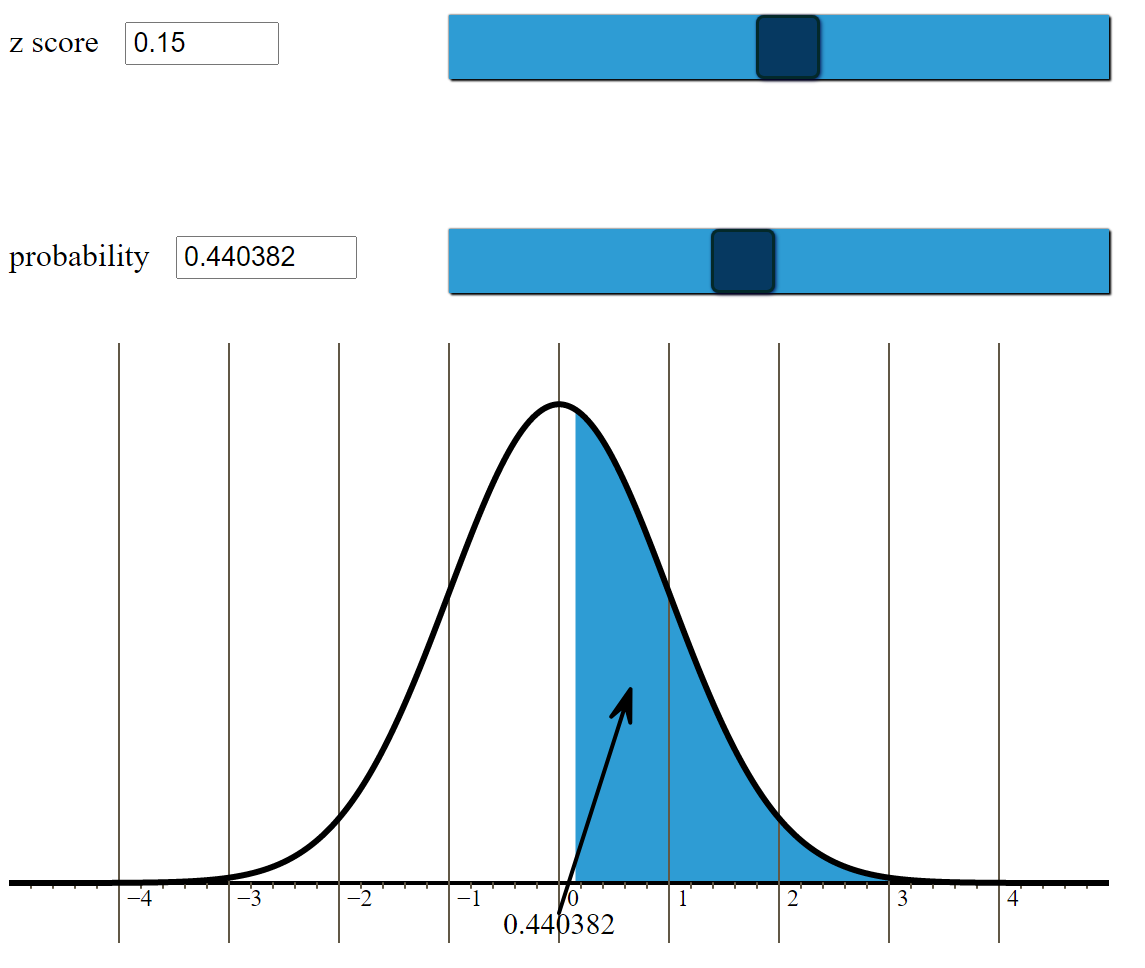
\includegraphics[width=3in]{z 0.15.PNG}
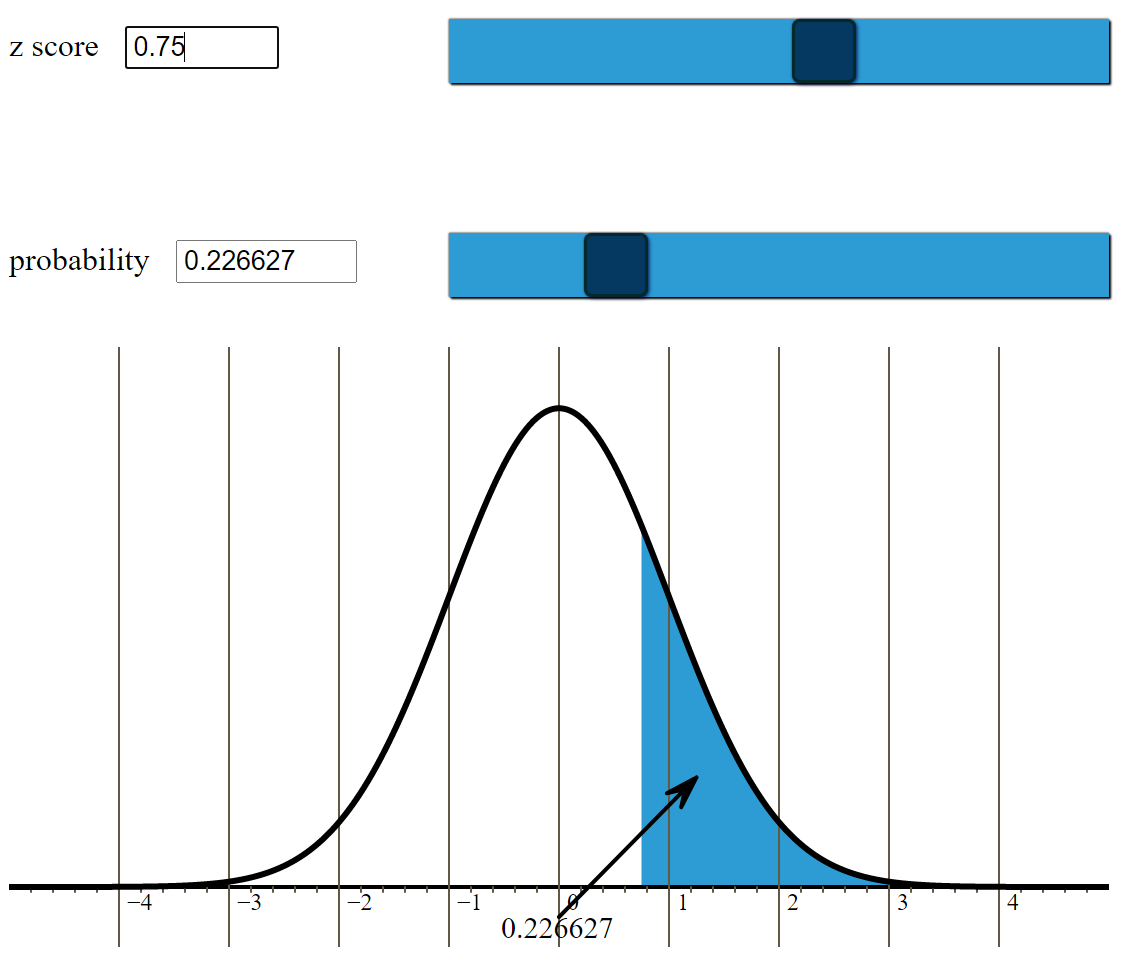
\includegraphics[width=3in]{z 0.75.PNG}

\nl Therefore, 
\begin{align*}
    \text{Table4}(0.15) - \text{Table4}(0.75) &= \P{Z > 0.15} - \P{Z > 0.75}\\ &= 0.4404 - 0.2266 \\ &= 0.2138
\end{align*}

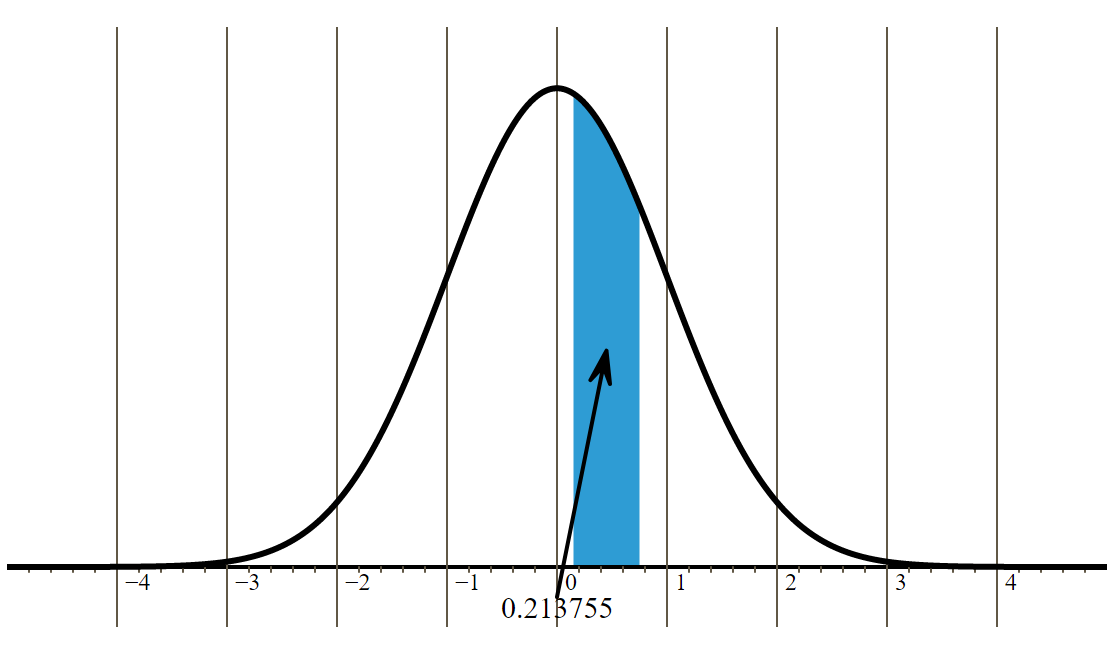
\includegraphics[width=6.25in]{7_4 normal area.PNG}

\disc* About $n$. Suprisingly, \say{large} $n$ doesn't need to be that large.\\Usually for any random variable $X$ and any distribution, then
$$\boxed{n \geq 30 \quad \text{is enough.}}$$

\noindent
That is, when $n \geq 30$, the CLT says $\normalDist{\mu}{\frac{\sigma^2}{n}}$ yields a good approximation of $\Xbar$.

\nl When $X$ is symmetric, unimodal, and continuous, $n = 4$ or $n = 5$ is often enough. 

\newpage
\addcontentsline{toc}{subsection}{Table 4: Normal Curve Areas}
\noindent\begin{center}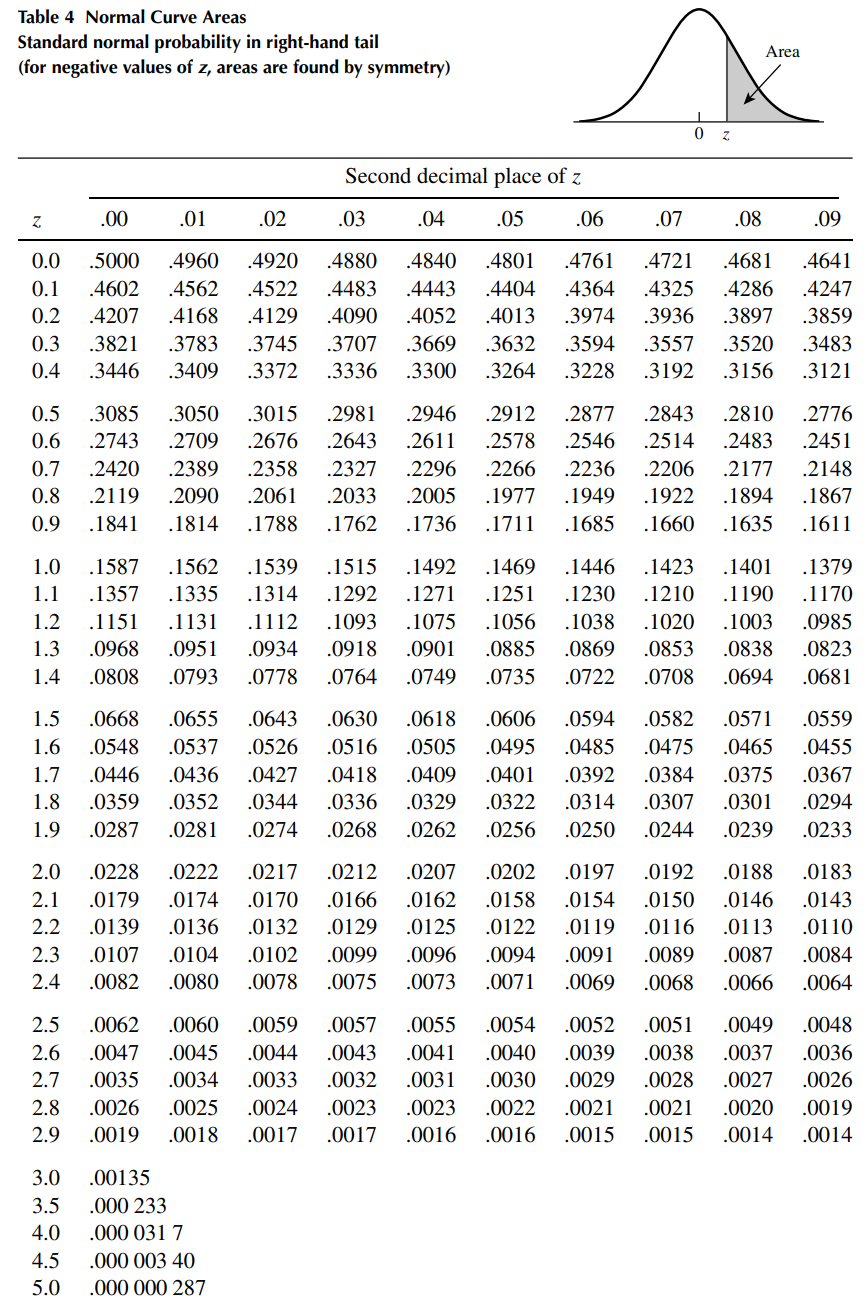
\includegraphics[width=6in]{Table4.png}
\end{center}
\chapter{Estimation}
\section{An Estimator}
We are seeking an unknown population parameter. General name of $\theta$ (e.g. $\mu$, $\sigma^2$, $\rho$, ...).

\nl The rule used to approximate or guess $\theta$ is called an \textbf{\underline{estimator}}. Any guess based on observations is called an \textbf{\underline{estimate}}.

\example Want $\theta = \mu$.

\vspace{0.2in}
Estimator: $\underbrace{\Xbar = \over{n} \sum x_i}_{\text{a function}}$

\vspace{0.15in}
Estimate: Given 7 observations, $Y_1, \dots, Y_7$, then
$\Ybar = \over*{7} \sum_1^7 Y_i$ is an \underline{estimate}.

\vspace{0.2in}
\nl This is an example of a \textbf{\underline{point}} estimator.

\nnl These are also \textbf{\underline{interval estimators}}.

\example Confidence interval, $\theta = \mu$.

$$\Xbar - SZ_x \leq \mu \leq \Xbar + SZ_x \qquad\iff\qquad |\Xbar - \mu | \leq SZ_x$$

\newpage
\section{The Bias and Mean Square Error of Point Estimators}
A start at trying to determine if a point estimator is any good.

\nl Let $\that$ be a point estimator for a parameter $\theta$. (e.g. $\theta = \mu, \quad \that = \Xbar$)
\begin{enumerate}[label=\textcircled{\raisebox{-1pt}{\arabic*}}]
    \item 
        One goal of a good estimator is that $E(\that) = \theta$ (e.g. by CLT, $\E{\Xbar} = \mu$)\\But this is not always the case.
        
        \defn If $\Eb*{\that}=\theta$, we say that $\that$ is an \textbf{\underline{unbiased}} point estimator.\\(e.g. $\Xbar$ is unbiased).

        \nl If $\that$ is a biased point estimator, we define the \underline{\textbf{bias}} to be
        $$\bias*{\that} = \Eb*{\that} - \theta$$
    
    \item 
        Another goal of a good estimator might be that its \say{spread} of observations is tightly packed (talking about variance), and hopefully near $\theta$.
        $$\text{spread}\, \Longrightarrow \text{variance}$$
        \defn* The \textbf{\underline{mean square error}} of $\that$ is
        $$MSE(\that) = E\brac{(\that - \theta)^2}$$
        Recall: $V[X] = E[X^2] - (E[X])^2$
        
        \nl \textbf{Corollary:}
        $$\MSE*{\that} = \Var*{\that} + \bigbrac{\bias*{\that}}^2$$
        \begin{proof}
            \begin{align*}
                \MSE*{\that} &= \Eb*{\that^2 - 2\that \theta + \theta ^2}\\
                &= \Eb*{\that^2} - 2\Eb*{\that\theta} + \Eb*{\theta ^2} \\
                &= \blue{\Eb*{\that^2}} - 2\Eb*{\that}\theta + \theta^2 \\
                &= \blue{\Eb*{\that^2} - \pars*{\Eb*{\that}}^2 + \pars*{\Eb*{\that}}^2} - 2\Eb*{\that}\theta + \theta ^2\\
                &= \Var*{\that} + \pars*{\Eb*{\that}-\theta}^2\\
                &= \Var*{\that} + \pars*{\bias*{\that}}^2
            \end{align*}
        \end{proof}
\remark We have decomposed MSE by:
$$\MSE*{\that} = \underbrace{\Var*{\that}}_{\text{Precision}} + \underbrace{\bias*{\that}^2}_{\text{Accuracy}}$$
\end{enumerate}
Idea of a \say{best} estimator is tricky. We'd like MSE to be as small as possible, but this is an impossible problem because MSE depends on the unknown $\that$.

\example (Population proportions). Want $p$.

\nnl To estimate, let
$$Y = \begin{cases} 
      1 & \text{\say{success}} \\
      0 & \text{\say{failure}} 
   \end{cases}$$
and $\{Y_i\}$ be an iid random sample.

\nnl \textbf{\red{Estimator 1:}} $\displaystyle \phat = \over{n}\sum Y_i = \Ybar$

\nl This sums the $\frac{\text{people said yes}}{\text{total people}}$

\recall* $\sum Y_i$ is $\text{binom}(n,p)$.

\nnl And for a Binomial Distribution, we know
$$\Eb{X} = np \wideand \Var{X} = npq = np(1-p)$$
Bias? Then what is the $\Eb*{\phat}$?
$$\Eb*{\phat} = \E{\over{n}\sum Y_i} = \over{n}\E{\sum Y_i} = \over{n}\cdot np = p$$
Because $\Eb*{\phat} = p$, then $\phat$ is an \underline{unbiased} estimator. For $\MSE*{\phat}$, we need $\Varb*{\phat}$:
$$\Varb*{\phat} = \Var{\over{n}\sum Y_i} = \pover{n}^2 \Var{\sum Y_i} = \pars{\over{n}}^2 np(1-p) = \frac{p(1-p)}{n}$$
Therefore,
\begin{align*}
    \MSE*{\phat} &= \Var*{\phat} - \bias*{\phat}^2\\
    &= \frac{p(1-p)}{n} + \underbrace{0^2}_{\text{\say{unbiased}}}
\end{align*}

\nnl \textbf{\red{Estimator 2: }} $\displaystyle \ptilde = \frac{\sum_1^n Y_i + 1}{n+2}$

$$n = 1, \qquad y = \begin{cases} 
      1\\
      0
   \end{cases} \qquad \ptilde = \begin{cases} 
      2/3 & \\
      1/3 \\
   \end{cases}$$
   $$n = 2, \qquad y = \begin{cases} 
      2\\
      1\\
      0
   \end{cases} \qquad \ptilde = \begin{cases} 
      3/4 \\
      2/4\\
      1/4
   \end{cases}$$
$$\Eb*{\ptilde} = \frac{\E{Y_i} + \E{1}}{n+2} = \frac{np+1}{n+2} = p + \frac{1-2p}{n+2} \neq p$$
Hence, $\ptilde$ is \underline{biased}. And,
$$\bias*{\ptilde} = \Eb*{\ptilde} - p = p + \frac{1-2p}{n+2} - p = \frac{1-2p}{n+2}$$

\nnl\textbf{Calc question:} What happens to $\Eb*{\ptilde}$ as sample size grows? ($\Eb*{\ptilde} \to p$)

\nnl Need
\begin{align*}
    \Var{\ptilde} &= \Var{\frac{\sum_1^n Y_i + 1}{n+2}} \\
    &=  \Var{\frac{\sum_1^n Y_i}{n+2} + \over{n+2}} \\
    &= \Var{\frac{\sum_1^n Y_i}{n+2}} \\
    &= \over{(n+2)^2} \Var{\sum_1^n Y_i} \\
    &= \frac{np(1-p)}{(n+2)^2}
\end{align*}
Then
\begin{align*}
    \MSE*{\ptilde} &= \Var{\ptilde} + \bias*{\ptilde}^2\\
    &= \frac{np(1-p)}{(n+2)^2} + \pars{\frac{1-2p}{n+2}}^2\\
    &= \frac{np(1-p) + (1-2p)^2}{(n+2)^2}
\end{align*}


\nl \textbf{Q:} Which estimator is better? \hspace{0.25in} \textbf{A:} \textit{it depends!}

\nnl Note that for both, $\MSE*{\ptilde}(n,p)$ are functions of $n$ and $p$. Let
$$\red{y=\MSE*{\ptilde}(n,p)} \wideand \blue{y=\MSE*{\phat}(n,p)}$$
\newpage
$$\text{fix } n = 10, \qquad p \in[0,1]$$
\begin{center}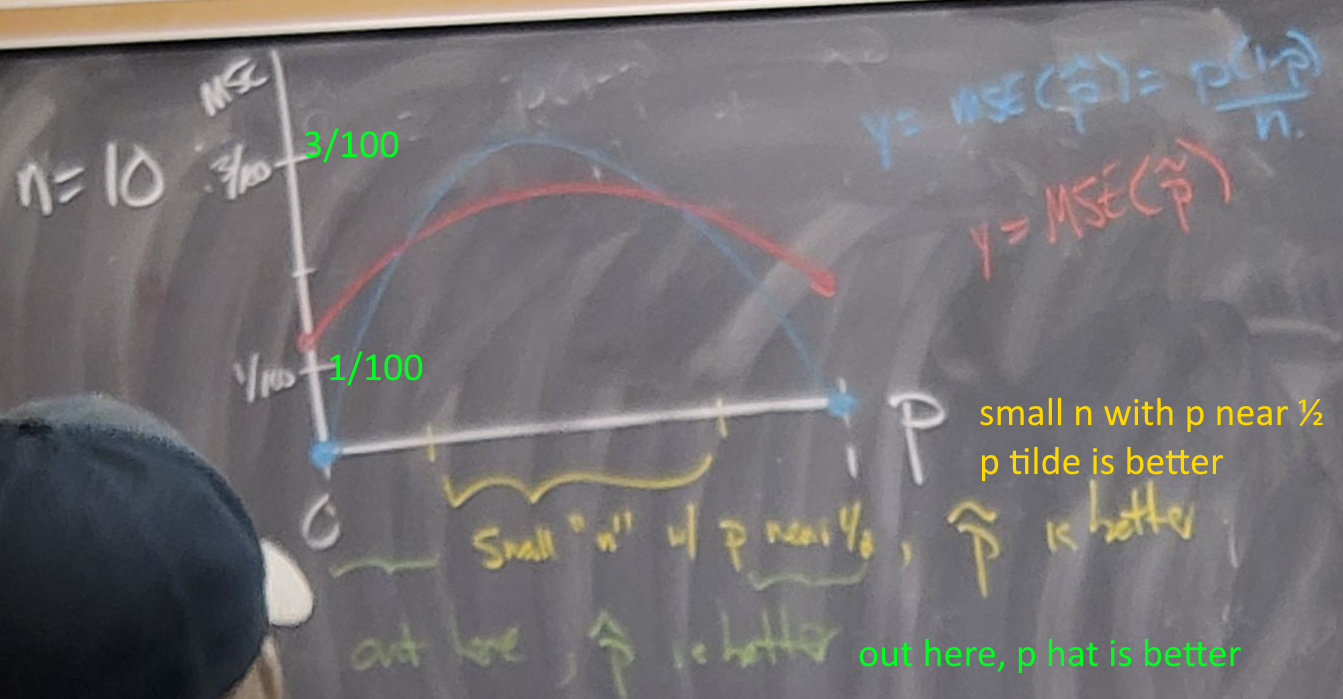
\includegraphics[width=15cm]{mse n 10.png}\end{center}

$$n = 25 \text{ and } 100 \qquad p \in [0,1]$$
\begin{center}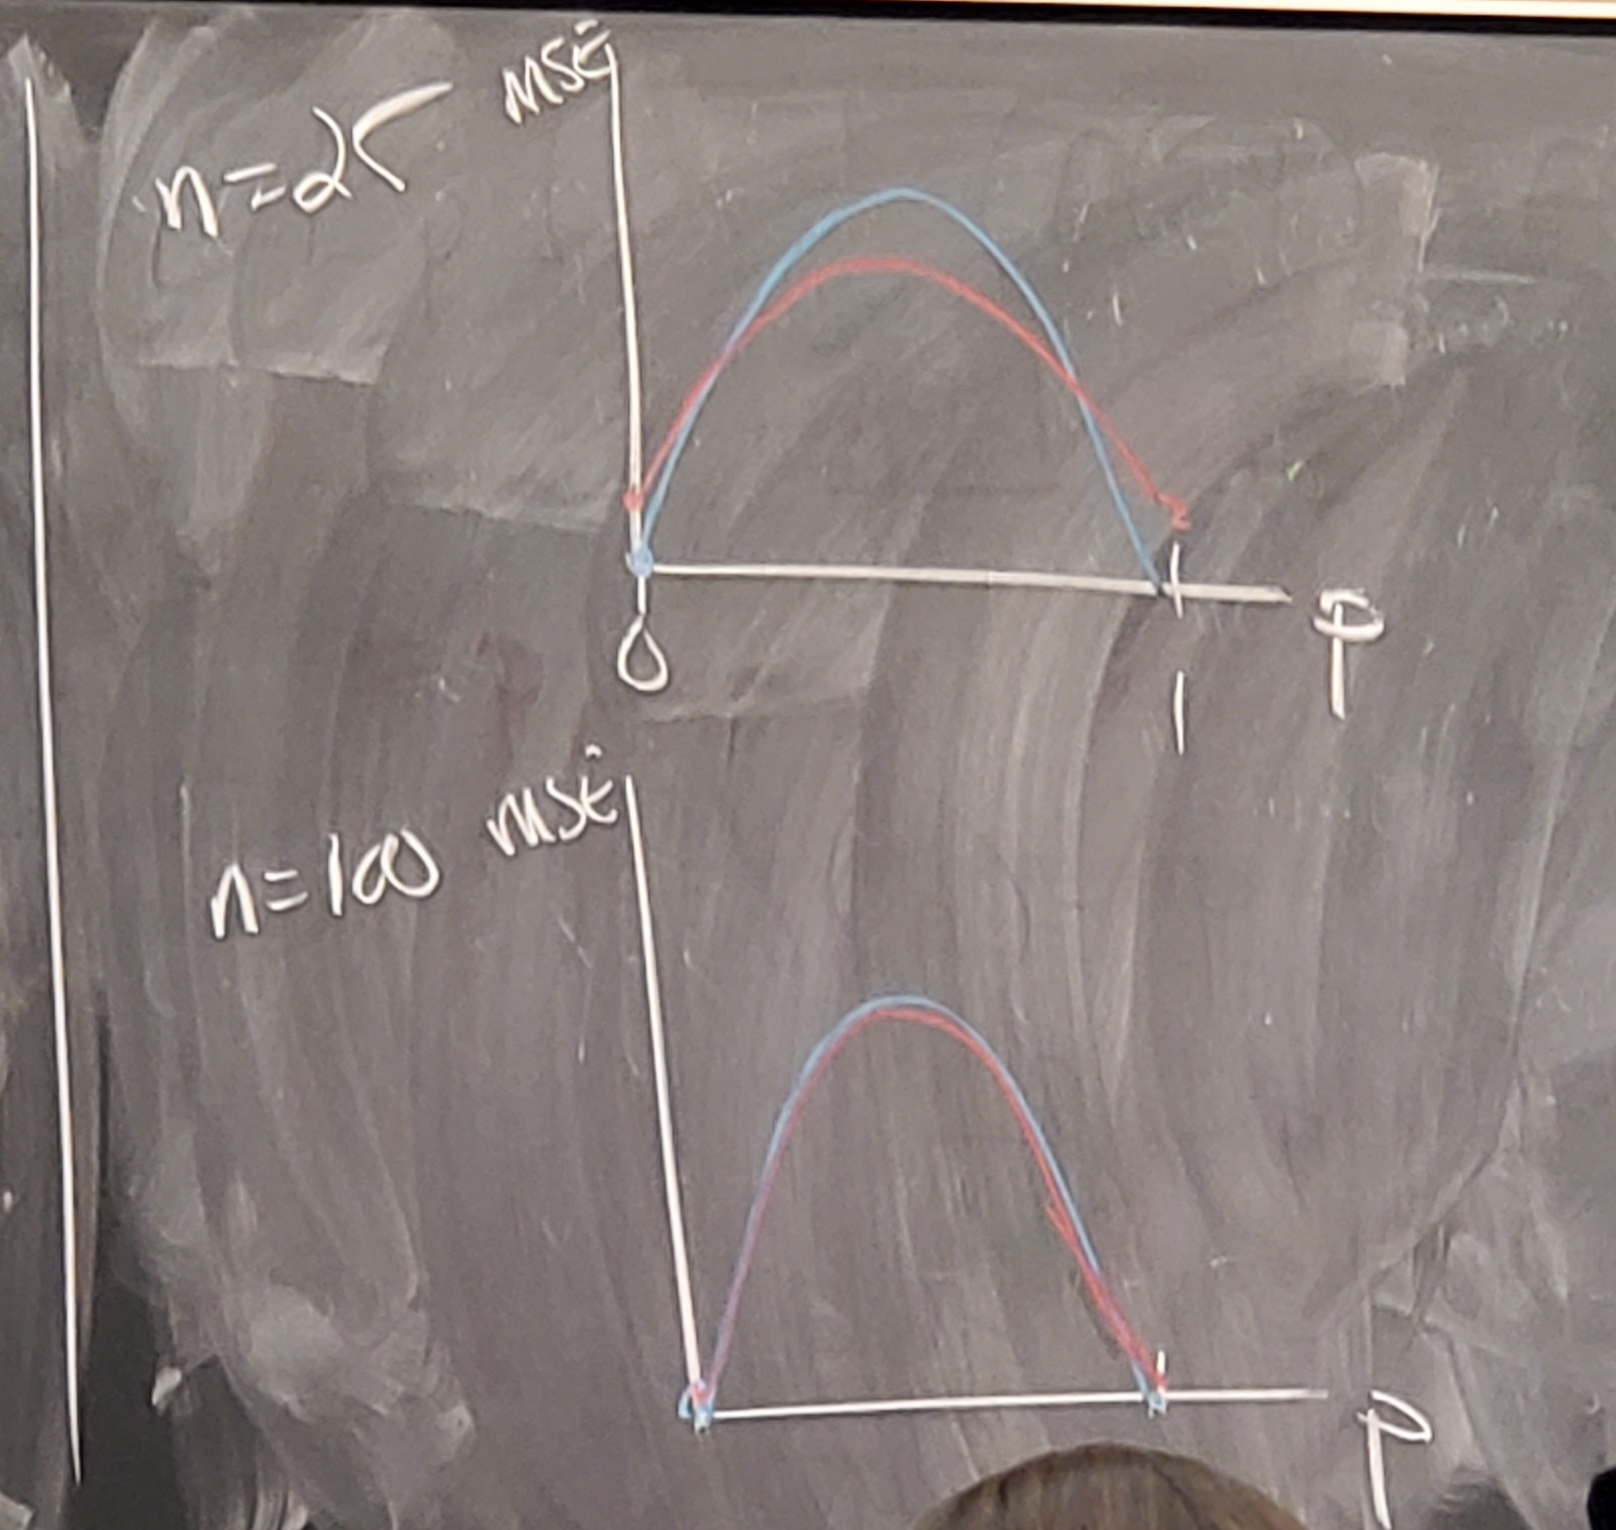
\includegraphics[width=4.5in]{mse 25 and 100.png}\end{center}
For larger $n$, they become indistinguishable.

\newpage
\section{Some Common Unbiased Point Estimators}
Table 8.1, page 397: Common unbiased estimator for $\mu,\quad \rho,\quad \mu_1 - \mu_2,\quad \rho_1 - \rho_0$.

\example Variance of a data set and the $n-1$.

\nnl Natural definition is $S^2 = \dfrac{1}{n}\sum \pars{X_i-\Xbar}^2$

\nnl Why do we use $n-1$?

\nl Check $\bias{S^2}$. Is $\E{S^2} = \sigma^2$? Let
$$\E{X} = \mu \qquad \text{and}\qquad \Var{X} = \sigma^2$$
and $\thru{X}$ iid random sample. Then,
\begin{align*}
    \E{S^2} &= \Eb{\over{n}\sum_{i=1}^{n} \pars{X_i - \Xbar}^2} \\
    &= \over{n}\underbrace{\Eb{\sum \pars{X_i^2 - 2X_i\Xbar + \Xbar ^2}}}_{\text{focus on this}}\\
    &= \over{n}\pars{\Eb{\sum X_i^2 - 2\sum X_i\Xbar + \sum \Xbar^2}}\\
    &= \over{n}\pars{\underbrace{\Eb{\sum X_i^2}}_{\text{\cir{1}}} - \underbrace{2\Eb{\sum X_i\Xbar}}_{\text{\cir{2}}} + \underbrace{\Eb{\sum \Xbar}^2}_{\text{\cir{3}}}} 
\end{align*}
\cir{1} and \cir{3} uses the same \say{trick} of $\Var{X} = \Eb{X^2} - \pars{\Eb{X}}^2 $. So,
\begin{align*}
    \text{Part \cir{1} } &= \Eb{\sum_{i=1}^{n} X_i^2} \\ 
    &= \sum \Eb{X_i^2}\\
    &= \sum \pars{\Var{X_i} + \pars{\Eb{X_i}}^2}\\
    &= \sum \pars{\sigma^2 + \mu^2} \\
    &= n\pars{\sigma^2 + \mu^2}
\end{align*}
\begin{align*}
    \text{Part \cir{3} } &= \Eb{\sum_{i=1}^{n} \Xbar^2} \\
    &= \sum \pars{\Var{\Xbar} + \pars{\Eb{\Xbar}}^2}\\
    &= \sum \pars{\frac{\sigma^2}{n} + \mu^2}\\ %since xbar dist by N(mu, sig^2/n)
    &= n \pars{\frac{\sigma^2}{n} + \mu^2} \\
    &= \sigma^2 + n \mu^2
\end{align*}
\begin{align*}
    \text{Part \cir{2} } &= -2\Eb{\sum_i X_i\pars{\over{n}\sum_j X_j}}\\
    &= -\frac{2}{n} \Eb{\sum_i \sum_j X_i X_j} \\%n^2 terms
    &= -\frac{2}{n} \Eb{\underbrace{\sum_i X_iX_j}_{n \text{ terms}} + \underbrace{\mathop{\sum\sum}_{i\neq j}  X_i X_j}_{n^2-n \text{ terms}}} \\
    &= -\frac{2}{n} \pars{\underbrace{\sum_i \Eb{X_i^2}}_{\text{this is part \cir{1} again}} + \underbrace{ \mathop{\sum\sum}_{i\neq j} \Eb{X_i X_j}}_{\text{covariance like}}}
\end{align*}
\recall
\begin{align*}
    \Cov(X_i,X_j) &= \Eb{\pars{X_i - \Xbar}\pars{X_j - \Xbar}} \\
    &= \Eb{X_iX_j} - \Eb{X_i}\Eb{X_j} 
\end{align*}
But iid, \say{i} for independent $\implies \Cov(X_i, X_j) = 0$. Therefore,
$$\Eb{X_i X_j} = \Eb{X_i}\Eb{X_j} = \mu \cdot \mu = \mu^2$$
\begin{align*}
    \text{Part \cir{2} } &= -\frac{2}{n}\Big(n(\sigma^2 + \mu^2) + (n^2 - n)\mu^2\Big)\\
    &= -2\brac{(\sigma^2+\mu^2) + (n-1)\mu^2}
\end{align*}
Substituting back into the original parts,
\begin{align*}
    \E{S^2} &= \over{n}\pars{\underbrace{\Eb{\sum X_i^2}}_{\text{\cir{1}}} - \underbrace{2\Eb{\sum X_i\Xbar}}_{\text{\cir{2}}} + \underbrace{\Eb{\sum \Xbar}^2}_{\text{\cir{3}}}} \\
    &= \over{n}\pars{\underbrace{n(\sigma^2+\mu^2)}_{\text{\cir{1}}} - \underbrace{2\Big( \pars{\sigma^2 + \mu^2} + (n-1)\mu^2 \Big) }_{\text{\cir{2}}} + \underbrace{\sigma^2 + n\mu^2}_{\text{\cir{3}}}} \\
    &= \over{n}\pars{n\sigma^2+n\mu^2 -2\sigma^2 -2\mu^2 -2(n-1)\mu^2+ \sigma^2 + n\mu^2} \\
    &= \over{n}\pars{n\sigma^2\color{red}{+n\mu^2} -2\sigma^2 \color{blue} -2\mu^2 \color{red}{-2n\mu^2} \color{blue} + 2\mu^2 + \sigma^2 \color{red}{+n\mu^2}} \\
    &= \over{n}\pars{n\sigma^2 -2\sigma^2 + \sigma^2} \\
    &= \over{n}\pars{n\sigma^2 -\sigma^2} \\
    &= \frac{\sigma^2(n-1)}{n} \\
    &\neq \sigma^2 
\end{align*}
Therefore, it is a \underline{biased} point estimate.

\nl To make an \underline{unbiased} estimator, rescale the summation of the natural definition...
$$S := \over{n-1} \sum_{i=1}^n \pars{X_i - \Xbar}^2$$

\newpage
\section{Evaluating the Goodness of a Point Estimator}
\defn* Given any $\that$, the exact (theoretical) error is defined as
$$\varepsilon = \big| \that - \theta \big|$$
Note that $\varepsilon$ is itself a random variable, and thus we can make probability statements about it. Obviously we want $\varepsilon$ to be small. Consider $\big| \that - \theta \big| < b$. We can make conclusions about
$$P\big(\big| \that - \theta \big| < b\big)$$

\noindent Chebyshev: $$P\big(\big| \that - \theta \big| < k\sigma\big) > 1 - \over{k^2}$$
\remark We call $\sigma = \sqrt{\sigma^2}$ the \bu{standard error} in stats.

\nl In practice, $k = 2$ is a common choice.
$$\P{\big| \that - \theta \big| < 2\sigma} > 1 - \over{2^2} = \frac{3}{4} = 0.75$$
In the real world, $2\sigma$ is usually much better than this (see Table 8.2) when the underlying distribution
$\that$ is symmetric and unimodal.

\nl Last working assumption for a few lectures: in real life we use $S^2 \approx \sigma^2$ (more later).

\example (Difference in means)

\nl 2 iid random samples:
$$n_1 = 100 \qquad \bar{Y_1} = \num[group-separator={,}]{26400} \qquad {S_1}^2 = \num{1440000}$$
$$n_2 = 200 \qquad \bar{Y_2} = \num{25100} \qquad {S_2}^2 = \num{1960000}$$

\nl Estimating difference in means $\mu_1 - \mu_2$. Here,
$$\bar{Y_1} - \bar{Y_2} = \underbrace{\num{26400} - \num{25100}}_{\text{a point estimate}} = \num{1300}$$
\recall $\sigma^2_{\Ybar_1 - \Ybar_2} = \dfrac{\sigma^2_1}{n_1} + \dfrac{\sigma^2_2}{n_2}$. Use $S^2_{\bar{Y_1} - \bar{Y_2}}$ to find a $2\sigma$ interval estimate:
$$\sigma^2_{\bar{Y_1} - \bar{Y_2}} \approx S^2_{\bar{Y_1} - \bar{Y_2}} = \frac{S_1^2}{n_1} + \frac{S_2^2}{n_2} \approx \frac{\num{1440000}}{100} + \frac{\num{1960000}}{200} = \num{22800}$$
$$\sigma_{\bar{Y_1} - \bar{Y_2}} \approx S_{\bar{Y_1} - \bar{Y_2}} = \sqrt{S_{\bar{Y_1} - \bar{Y_2}}^2} = \sqrt{\num{22800}} \approx 151$$

\nl Therefore, a $2\sigma$ interval estimate for $\mu_1 - \mu_2$ is $1300 \pm \green{2}(151) \implies 1300 \pm 302 \text{ or } (998, 1602)$

\newpage
\section{Confidence Intervals}
Goal: Take interval estimates from $\S$8.4 but make more precise comments about the probability $\P{\big| \that - \theta \big| < k\sigma}$
$$-k\sigma < \that-\theta < k\sigma\quad \iff \quad \that - k \sigma < \theta < \that + k\sigma$$

\nl Consider
$$\P{\that_L \leq \theta \leq \that_u} = 1 - \alpha$$
$\that_L$ and $\that_U$ are the lower and upper \bu{confidence limits}, respectively.

\nl $1-\alpha$ is the \bu{confidence coefficient}.

\example

\nl Want $9\%$ CI, chose $\alpha = 5\%$ when we know how $\that$ is distributed. We can use standardization methods to find the limits.

\nnl Two sided confidence interval:
$$\P{\that_L \leq \theta \leq \that_u} = 1 - \alpha$$
One sided:
$$\P{\that_L \leq \theta} = 1 - \alpha \qquad \P{\that_U \geq \theta} = 1 - \alpha$$
\textbf{Discussion:} The pivotal method for finding confidence intervals.
\begin{enumerate}[label=\textcircled{\raisebox{-1pt}{\arabic*}}]
    \item We know how a r.v. $Y$ is distributed, but \underline{not} some underlying parameter $\theta$.
    \item Using a distribution of an estimator $\that$, we convert to a probability distribution that does not depend on $\theta$ (standardizing).
\end{enumerate}

\example

\nl $\Xbar$ distributed $\normalDist{\mu}{\frac{\sigma^2}{n}}$, via
$$Z = \frac{\Xbar - \mu}{\sqrt{\sigma^2/n}} \quad \Longrightarrow \underbrace{N(0,1)}_{\text{Independent of $\mu$}}$$

\nl We use $N(0,1)$ to rescale the limits of $\that_L$ and $\that_U$.

\example

\nl $\yn$ an iid random sample of size $n$ from a uniform distribution on the interval $(0,\; \theta)$.

\nnl We want an estimate for $\theta$, use
$$\that = \max{\yn}$$
We know how $\that$ is distributed, but it is clearly dependent on $\theta$. 
$$\text{For } \, Y_i\;, \quad f(y) = \over{\theta}$$
$$\implies F(y) = \P{Y \leq y} = \int_0^y \over{\theta} = \frac{y}{\theta}, \qquad y \in [0,\theta]$$

$$F(y) =
\begin{cases} 
      0 & y < 0 \\
      y/\theta & y \in [0, \theta]\\
      1 & y > \theta\\
\end{cases}$$

\nl The max order stat $\that$ has CDF:
\begin{align}
    \P{\that < w} &= \P{Y_1 \leq w,\; Y_2 \leq w,\; \dots,\; Y_n \leq w} \notag\\
    &= [\P{Y \leq w}]^n \notag\\
    &= \begin{cases} 
        0 & w < 0 \\
        (w/\theta)^n & w \in [0, \theta]\\
        1 & w > \theta\\
    \end{cases} \notag
\end{align}

\nl Use a change of variables to find an associated pivotal distribution: $U = \dfrac{\that}{\theta}$

\nl The CDF of U,

\begin{align}
       \P{U\leq u} &= \P{\frac{\that}{\theta} \leq u} \notag\\
       &= \P{\that \leq \theta u}\notag\\
       &= \pars{\frac{\theta u}{\theta}}^n \notag\\
       &= u^n \text{ for } u \in [0,1]\notag
\end{align}
$$F(u) = 
\begin{cases} 
      0 & u < 0 \\
      u^n & u \in [0, 1]\\
      1 & u > 1\\
\end{cases}$$

\nl\color{red}Pivotal CDF of $u$, no longer depends upon $\theta$.\color{black}

\nl \color{ggreen} We use $U$'s CDF to construct a confidence interval.\color{black}

\nl Goal: Find a $95\%$ lower confidence interval for $\theta$.
Want:
$$\P{\underbrace{\that_L \leq \theta}_{\text{\color{red}One-sided C.I.}}} = 0.95$$
Using $U$'s CDF: \hspace{0.1in} $\P{U\leq u} = 0.95 \quad \iff \quad u^n = 0.95$
$$\color{red}u = \sqrt[n]{0.95} = (0.95)^{1/n}$$
Then,
\begin{align}
    \P{\frac{\that}{\theta} \leq (0.95)^{1/n} } &= 0.95\notag\\
    \P{\frac{\that}{(0.95)^{1/n}} \leq \theta} &= 0.95\notag
\end{align}
But $\that = \operatorname{max}(\yn) = Y_{(n)}$

\nl So, our $95\%$ confidence interval is
$$\frac{Y_{(n)}}{(0.95)^{1/n}} \leq \theta.$$

\example

\nl For a random sample
$$\underbrace{0.76, 0.88, 1.68, 1.74, 1.78}_{\textstyle \setGreen n\,=\, 5}$$
$$Y_{(5)} = 1.78$$
A $95\%$ C.I. for $\theta$ is given by $n=5, \; Y_{(5)} = 1.78$
$$\frac{1.78}{(0.95)^{1/5}} \leq \theta$$
$$\frac{1.78}{0.98979} \leq \theta$$
$$1.798 \leq \theta$$

\newpage
\section{Large Sample Confidence Intervals}
   The unbiased point estimates for $\mu,\; \rho,\; \mu_1 - \mu_0,\; \rho_1 - \rho_2$ all have near Normal distributions by the Central Limit Theorem.
   
   \nl Moreover, using
   $$Z = \frac{\that-\theta}{\sigma_{\that}}$$
   $Z$ is a pivotal quantity $N(0,1)$.

   \nnl For two-sided confidence intervals,
   $$\P{-Z_{\alpha/2} \leq Z \leq Z_{\alpha/2}} = 1 - \alpha$$
   
   \nl \begin{center}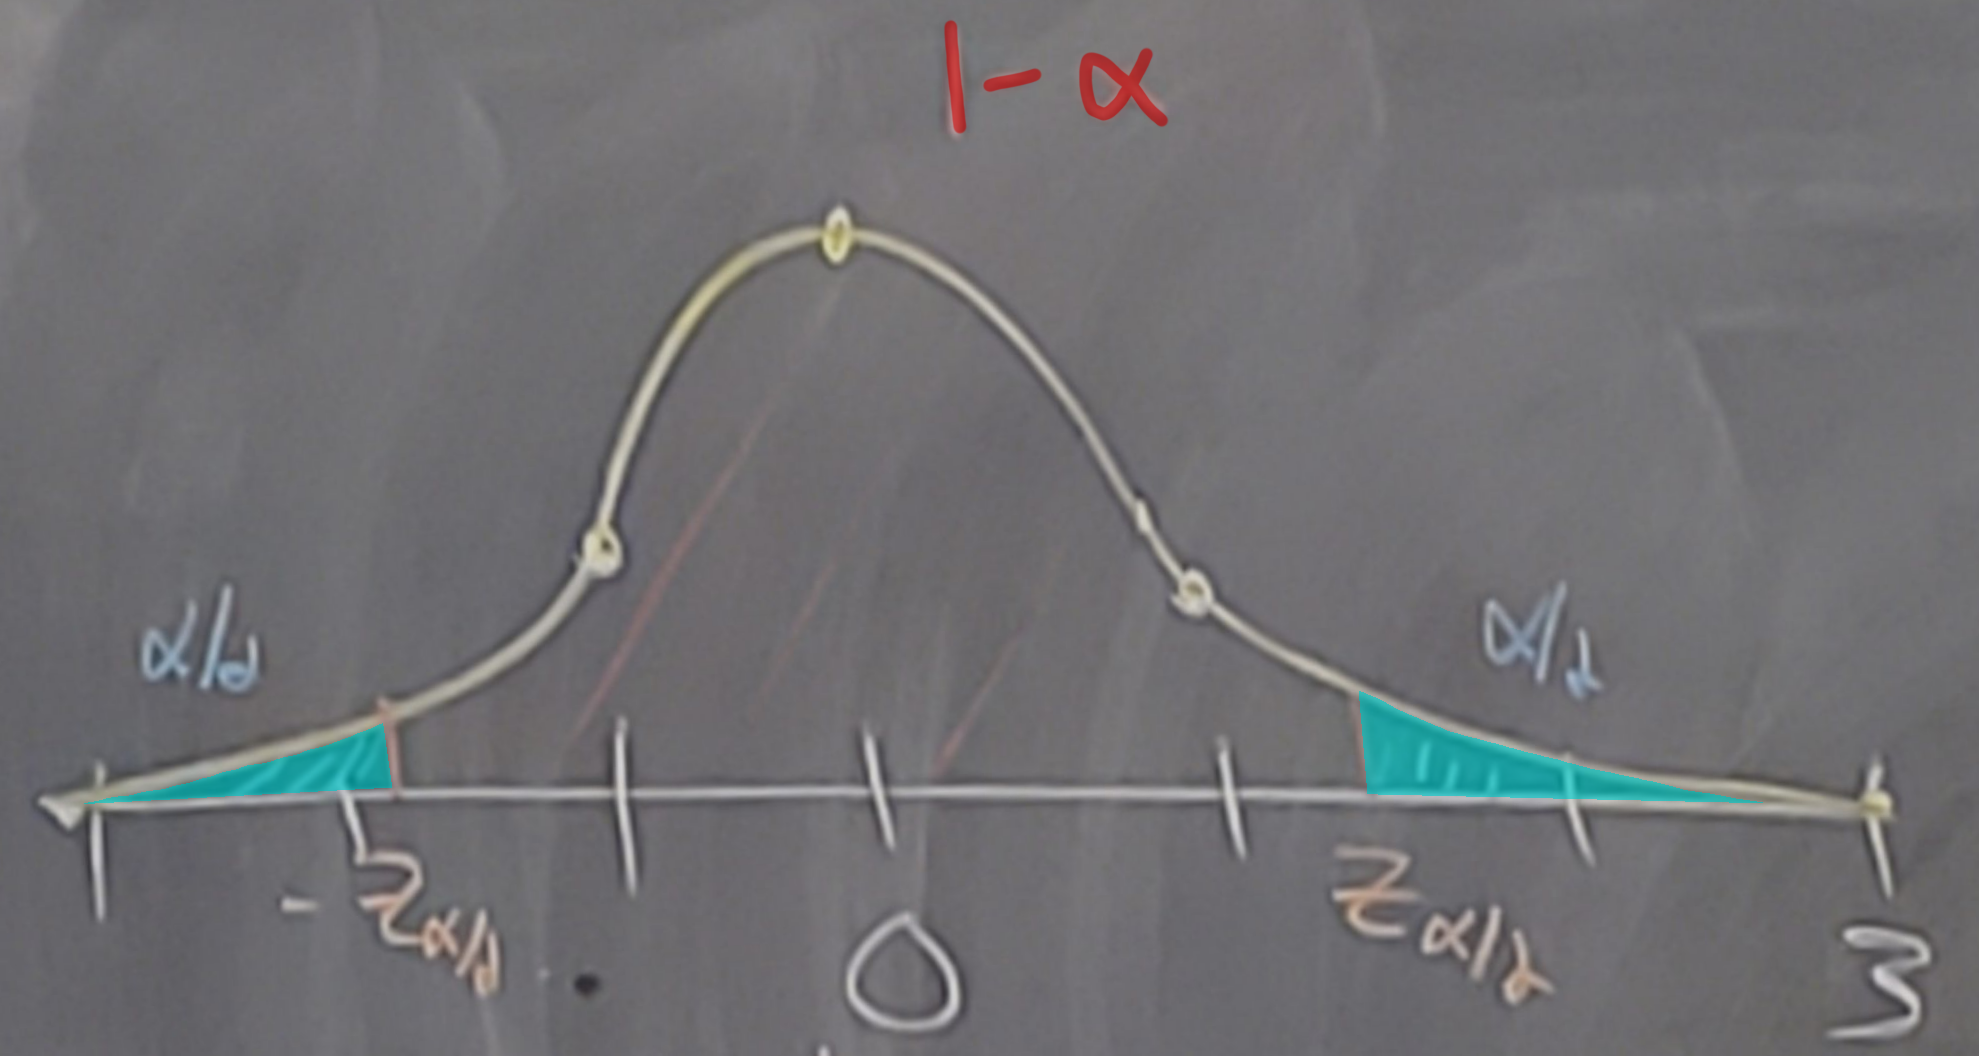
\includegraphics[width=6in]{alphaover2.png}\end{center}

   \nl Some common standard errors:
   \begin{align}
    90\% \text{ C.I. } \,& \Longrightarrow Z_{0.05} = 1.645\notag\\
    95\% \text{ C.I. } \, &\Longrightarrow Z_{0.025} = 1.960\notag\\
    99\% \text{ C.I. } \, &\Longrightarrow Z_{0.005} = 2.576\notag
   \end{align}
   Then
   $$-Z_{\alpha/2}  \leq Z \leq Z_{\alpha/2}$$
   $$-Z_{\alpha/2}  \leq \frac{\that-\theta}{\sigma_{\that}} \leq Z_{\alpha/2}$$
   $$-Z_{\alpha/2} \sigma_{\that}  \leq \that-\theta \leq Z_{\alpha/2} \sigma_{\that}$$
   $$-Z_{\alpha/2} \sigma_{\that} - \that \leq -\theta \leq Z_{\alpha/2} \sigma_{\that} - \that$$
   $$\underbrace{\that - Z_{\alpha/2} \sigma_{\that}}_{\that_L} \leq \theta \leq  \underbrace{\that + Z_{\alpha/2} \sigma_{\that}}_{\that_U}$$
           %green box around that with text 1-alpha confidence interval
           
    \noindent Of course, we don't know $\sigma_{\that}$ exactly. For \say{large} samples, we can use $\sigma_{\that} \approx S_{\that}$.
    
    \example*
    $$\Xbar = 19.07 \hspace{1in} S^2 = 10.60 \hspace{.75in}\text{with}\hspace{0.25in} n = 32$$
    \textit{Recall:} For \say{large} samples ($n \geq 30$), $\Xbar$ nearly distributed by $N(\mu, \sigma^2_{\Xbar}) \approx N(\mu, \frac{10.60}{0.32})$.
    \\For a $95\%$ CI for $\mu$,
    $$\sigma_{\Xbar} \approx \sqrt{\frac{10.60}{0.32}} \approx 0.576$$
    Here, $\alpha = 0.05$ and $\frac{\alpha}{2} = 0.025$. So $\Xbar \pm Z_{0.025} \sigma_{\Xbar}$, thus
    $$19.07 \pm (1.96)(0.576)$$
    $$\Rightarrow 19.07 \pm 1.128 \quad \text{or} \quad (17.94,\, 20.20)$$

    \disc* Differences in population proportions.

    \nl Estimating $p_1 - p_2$ by $\phat_1 - \phat_2$ for samples of size $n_1$ and $n_2$ respectively.
    \begin{align}
        \that\,\pm\, Z_{\alpha / 2} \sigma_{\that} &\quad\implies\quad \phat_1 - \phat_2 \,\pm\, Z_{\alpha/2} \sqrt{\sigma_{\phat_1}^2 + \sigma_{\phat_2}^2 } \notag\\
        &\quad\implies\quad \phat_1 - \phat_2 \,\pm\, Z_{\alpha/2} \underbrace{\sqrt{\frac{p_1q_1}{n_1}+\frac{p_2q_2}{n_2}}}_{\substack{\text{Depends on the} \\ \text{unknowns } p_1,\; p_2}}\notag
    \end{align}

    
    \nl Two standard fixes:
    \begin{enumerate}[label=\textcircled{\raisebox{-1pt}{\arabic*}}]
        \item $pq = p(1-p) \leq 1/4$\\
            Easy to show by calculus. Yields a \say{max} error via
            $$\sqrt{\over{4n_1}+\over{4_n2}}.$$
            However, in practice we use \cir{2} as smaller confidence intervals are desirable.
        
            \vspace{0.35in}
            \item When $n_i$ is large enough, we can use $\phat_1$ for $p_i$.
        
        \nl The $1-\alpha$ confidence interval is
        $$\phat_1-\phat_2 \,\pm\, Z_{\alpha/2}\sqrt{ \frac{\phat_1(1-\phat_1)}{n_1}   \, + \, \frac{\phat_2(1-\phat_2)}{n_2}  } $$
    \end{enumerate}
           

\newpage
\section{Selecting the Sample Size}

For our C.I. we have $\that\pm Z_{\alpha/2}\sigma_{\that}$
    \begin{itemize}
        \item $\sigma_{\that}$ is the standards error
        \item $E = Z_{\alpha/2}\sigma_{\that}$ is the error bounds of our C.I.
    \end{itemize}
    In real world, we choose our confidence level $1-\alpha$ and/or the error $E$ ahead of time. This leads to the problem of choosing an appropriate sample size $n$.
    
    \example For $\bar{X}, \dots$ distributions is $\normalDist*$.
    $$\sigma_{\Xbar} = \sqrt{\sigma^2/n} \qquad \text{and} \qquad E = Z_{\alpha/2} \sqrt{\sigma^2/n}$$
    $$\longleftrightarrow\quad n = \frac{Z_{\alpha/2}\sigma^2}{E^2}$$
    For desired $E$, we need to choose
    $$n \geq \left\lceil \frac{Z_{\alpha/2}\sigma^2}{E^2}\right\rceil$$
    Another issue: We don't really know ${\sigma_{\that}}^2$ and maybe not even $Z_{\alpha/2}$.

    \begin{enumerate}[label=\textcircled{\raisebox{-1pt}{\arabic*}}]
        \item For $Z_{\alpha/2}$, we have seen that the empirical rule $2\sigma$ usually works for large $n$.
        \begin{center}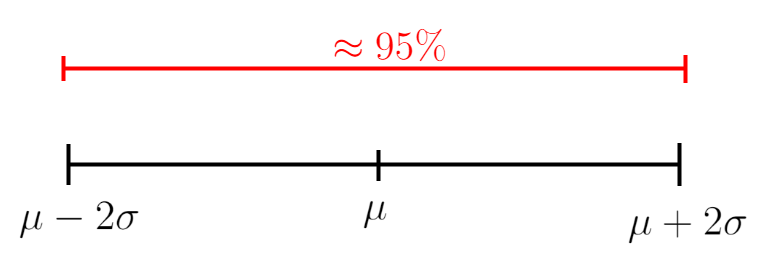
\includegraphics[width=4in]{2 sigma.png}\end{center}

        \item For $\sigma_{\that}$, either
        \begin{enumerate}[label=\textbf{{\alph*}.)}]
            \item Use old data or a \say{pilot} sample $S^2$
            \item Use $\over{4}$ the spread of the data set, i.e.,
            $$\sigma_{\that} \approx \over{4} \big( \operatorname{max}(Y_i)-\operatorname{min}(Y_i)\big) $$
        \end{enumerate}
    \end{enumerate}
    However, for proportions we can do even better.

    \example Proportions. For 
    $\phat = \dfrac{\displaystyle \sum Y_i}{n} \hspace{0.25in} \text{(relative frequency)}$,  
    $\;\phat$ distributed $N\pars{p, \dfrac{pq}{n}}$
    $$E = Z_{\alpha/2} \sqrt{\frac{pq}{n}} \hspace{.5in} \longleftrightarrow \hspace{0.5in} n \geq \left\lceil \frac{Z_{\alpha/2}^2p(1-p)}{E^2}\right\rceil $$
    Again, since $p(1-p) \leq \dfrac{1}{4}$ on $[0,\,1]$, we choose $n \geq \dfrac{Z_{\alpha/2}^2}{4E}$

    \newpage \noindent \example* Public opinion polls ($\pm 3\%$)

    \nnl For a 95\% Confidence interval,
    $$Z_{\alpha/2} = 1.960 \qquad \text{and} \qquad n \geq \ceiling{\frac{1.96^2}{4(0.03)^2}} = 1068$$

    \nnl For a 99\% Confidence interval,
    $$Z_{\alpha/2} = 2.576 \qquad \text{and} \qquad n \geq \ceiling{\frac{2.576^2}{4(0.03)^2}} = 1844$$

\newpage
\section{Small-Sample Confidence Intervals for $\mu$ and $\mu_1 - \mu_2$}

\nl So for for $\Xbar$ when $n$ is large, we have used
$$\frac{\that - \mu}{\sigma \big/ \sqrt{n}} \approx \frac{\that - \mu}{S \big/ \sqrt{n}}$$
\begin{center}{\color{red} for small $n$, no longer precise enough.}\end{center}

\nl But we set ourselves up for this issue back in Chapter 7.

\recall* We know $\displaystyle Z = \frac{\that - \mu}{\sigma \big/ \sqrt{n}}$ is distributed $N(0,\;1)$
\\and $\displaystyle V = \frac{(n-1)S^2}{\sigma^2}$ is distributed $\chi^2$ with $n-1$ df and $Z$ and $V$ are independent. Let
\begin{align*}
    T &= \frac{\Xbar - \mu}{S \big/ \sqrt{n}}\\
    &= \frac{\Xbar - \mu}{S \big/ \sqrt{n}} \cdot \over{s \big/ \sigma}\\
    &= \frac{\Xbar - \mu}{\sigma \big/ \sqrt{n}} \cdot \over{\sqrt{S^2 \big/ \sigma^2}}\\
    &= Z \cdot \frac{1}{\sqrt{\displaystyle\frac{(n-1)S^2}{\sigma^2} \bigg/ (n-1)}}
\end{align*}
We write $T = \dfrac{Z}{\sqrt{V \big/ r}}$ where $r = (n-1)$. \\\red{$T$ is the product of 2 pivotally distributed independent random variables.}

\defn We say $T$ has a $t$-sampling distribution ($t$-dist'n) with $(n-1)$ degrees of freedom and its pdf is given by
$$f_T(t) = \dfrac{\varGamma \pars{\dfrac{r+1}{2}}}{\sqrt{\pi r} \cdot \varGamma \pars{\dfrac{r}{2}}} \cdot \pars{1 + \dfrac{t^2}{r}}^{\textstyle-\frac{r+1}{2} }$$

\nl \textit{Remarks:}
\begin{enumerate}[label=\textcircled{\raisebox{-1pt}{\arabic*}}]
    \item We won't work with $f_T(t)$ explicity. \red{Note this distribution is pivotal... }  Independent of $\mu$ and $\sigma^2$. We pick our $t_{\alpha/2}$ from Table 5, page 849. Notice $\df = r = n-1 \geq 30$ are $Z$-scores:
    
    \nl To do so we need $\alpha$ and d.f. $= n-1$
    \newpage
    \addcontentsline{toc}{subsection}{Table 5: $t$-Distributions}
    \notab{\begin{center}
        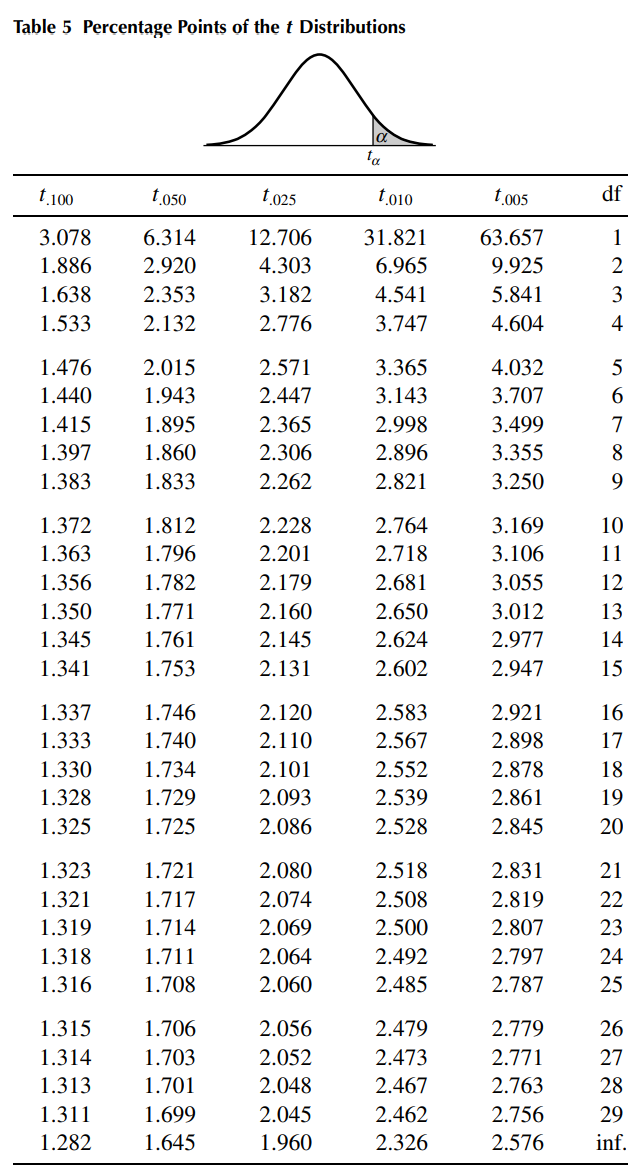
\includegraphics[width=5in]{Table5.png}
        \end{center}}
    \newpage
    \item $t$-distribution looks like \say{fat tailed} Normal Curves:
    \notab{\begin{center}
        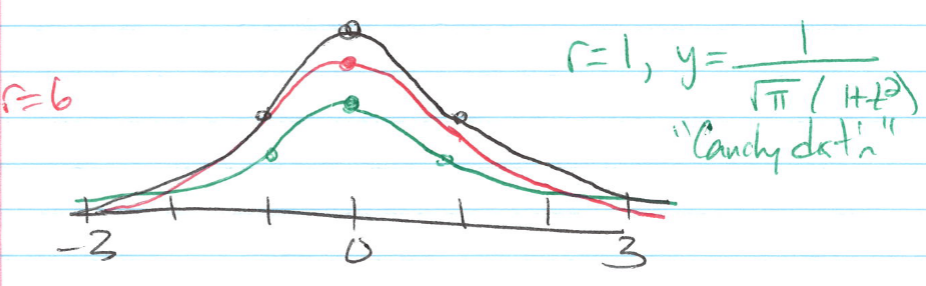
\includegraphics[width=5in]{8_8_rmk2.png}
        \end{center}}
    FACT: as $r \to \infty$, the D-distribution $\to N(0,\,1)$.

    \nl FUN FACT: Cauchy distribution is \say{famous}.
    $$r=1,\qquad \mu_T = 0, \quad \text{but} \quad \sigma^2_T = \infty$$

    \disc*    Small $n$ Confidence Interval.

    \nl For 2 sided, $T = \dfrac{\Xbar - \mu}{S \big/ \sqrt{n}}$
    \notab{\begin{center}
        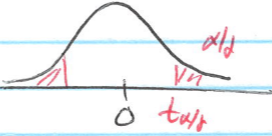
\includegraphics[width=2in]{8_8_im3.png}
        \end{center}}
    $$\P{-t_{\alpha/2} \, \leq \, T\, \leq t_{\alpha/2}} = 1 - \alpha$$
    $$\implies \Xbar \pm t_{\alpha/2} \pars{\dfrac{S}{\sqrt{n}}}$$

    \example $\quad n = 10, \qquad \Xbar = 3.22, \qquad S = 1.17$

    \nl Find a 95\% confidence interval for $\mu$.

    \nl Table 5: \hspace{.5cm} 95\% $\longrightarrow t_{0.025}$ with $\text{df} = (n-1) = 10-1 = 9$.

    \nl Use $t_{0.025} = 2.262$ and then $\Xbar \pm t_{0.025} \pars{\dfrac{S}{\sqrt{n}}} \implies 3.22 \pm (2.262) \pars{\dfrac{1.17}{\sqrt{10}}}$
    $$3.22 \pm 0.84 \; \implies \; (2.38,\;4.06)$$
    \newpage
    BONUS MATH: From the t-distribution.

    \nl For the math curious, it comes down to a fancy change of variables.

    \nl Recall from last semester, of $X$, $Y$ are independent, the joint pdf is $f(x,y) = f_x(x)f_y(y)$.

    \nl Here, $T = Z \pars{\dfrac{V}{r}}^{\textstyle  -\frac{1}{2} }$ and $Z$, $V$ are independent (as $\Xbar$ and $S$ are by Fisher's theorem).

    \nl To derive $f_T$, start with the join pdf of $Z$ and $Y$, a $\chi^2$ distribution of $r$ degrees of freedom. Then,
    $$f(y,z) = \frac{1}{\varGamma \pars{\dfrac{r}{2}} 2^{\scriptstyle r\scriptstyle/2 }} \cdot \displaystyle y^{\textstyle \frac{r}{2} \scriptstyle - 1} \cdot \exp\brac{-\frac{r}{2}} \cdot \over{\sqrt{2\pi}} \cdot \exp \brac{ \dfrac{Z^2}{2}} \qquad y\in(0,\;\infty), \quad Z \in \R$$
    Then let $t = Z \pars{\dfrac{V}{r}}^{\textstyle -\frac{1}{2}}, \qquad V = y$.
    \begin{align*}
        \P{Y<y,\; Z<z} &= \int_{-\infty}^{y} \int_{-\infty}^{z} f(y,z)\,dy\,dz\\
        &= \int_{-\infty}^{T} \int_{-\infty}^{V} f\Big(y(t,v),\, z(t,v)\Big) \red{\underbrace{\detx{Y_t}{Y_v}{Z_t}{Z_v}^{-1}}_{\text{Jacobian}}}  dt\,dv
    \end{align*}
    \setGreen Recall from MTH 420, for $u = h(x)$:
    $$\int_a^b f(x)\,dx = \int_{h(a)}^{h(b)} f\big(h^{-1}(a)\big) \frac{d}{dx}\Big(h^{-1}(u)\Big)\,du$$\setBlack

    \disc    Difference in means, small sample.

    \nl Start with $X,\; E[\,X\,] = \mu_x, \quad V[\,X\,] = \sigma^2_x$, \red{(Normal)}.\\
    And a r.v. $Y,\; E[\,Y\,] = \mu_y, \quad V[\,Y\,] = \sigma^2_y$, \red{(Normal)}.

    \nl Now we take 2 different iid random samples, which yields
    $$\Xbar \text{ and } S_{\Xbar}^2 \quad \text{with } \; n_1$$
    $$\Ybar \text{ and } S_{\Ybar}^2 \quad \text{with } \; n_2$$
    We have the unbiased estimator $\Xbar - \Ybar$ with $V(\Xbar - \Ybar) = \dfrac{\sigma^2_{\Xbar}}{n_1} + \dfrac{\sigma^2_{\Ybar}}{n_2}$. Then,
    $$Z = \frac{(\Xbar - \Ybar) - (\mu_x - \mu_y)}{\displaystyle \sqrt{\dfrac{\sigma^2_{\Xbar}}{n_1} + \dfrac{\sigma^2_{\Ybar}}{n_2}}} \quad \text{\red{a pivotal quantity.}}$$

    \nl Again, for small $n_i$, using $S_i \approx \sigma_i$ is not precise enough.

    \nl \red{Assumption: Let $\sigma_{\Xbar} = \sigma^{\Ybar}$. Thus}
    $$Z = \frac{(\Xbar - \Ybar) - (\mu_x - \mu_y)}{\displaystyle \sigma \sqrt{\dfrac{1}{n_1} + \dfrac{1}{n_2}}} \quad \text{\red{a pivotal quantity.}}$$

    \nl \red{Now we need to construct a point estimator for $\sigma$.}

    \nnl \textbf{Idea:} Try a \say{pooled} estimator.
    $$S_p^2 = \dfrac{\displaystyle \sum(X_i - \Xbar)^2 + \sum(Y_i-\Ybar)^2}{\red{r}}$$
    $$S_p^2 = \dfrac{\displaystyle (n_1-1) S_{\Xbar}^2 + (n_2-1) S_{\Ybar}^2}{\red{r}}$$
    Claim: $S_p^2$ is unbiased when $r = \big[ \red{(n_1-1)} + \red{(n_2-1)} \big] = n_1 + n_2 -2$. (i.e. $E[\,S^2_p\,] = \sigma^2 $)

    \nl \textit{Reason:} It is really the same computation as when we showed that $E[\,S^2\,] = \sigma^2$ when $S = \dfrac{1}{n-1}\displaystyle \sum(X_i-\Xbar)^2$\\Or, we can think about this as a product distribution of 2 independent $\chi^2$ distributions. One with $n_1-1$ df and another with $n_2-1$ df. Then (like with mgfs) the product distribution is $\chi^2$ with $n_1 - 1 + n_2 - 1$ df.

    \defn The \bu{pooled estimator} is
    $$S_p^2 = \dfrac{\displaystyle \sum(X_i - \Xbar)^2 + \sum(Y_i-\Ybar)^2}{n_1 + n_2 -2}.$$
    This is unbiased, and now we can define the t-statistic for $\mu_X - \mu_Y$ as
    $$T = \dfrac{(\Xbar-\Ybar)-(\mu_X-\mu_Y)}{S_p \displaystyle \sqrt{\dfrac{1}{n_1} + \dfrac{1}{n_2}}}.$$
    Which has $n_1 + n_2 - 2$ degrees of freedom.
\end{enumerate}

\newpage
\section{Confidence Intervals for \(\sigma^2\)}

\nl We have $S = \dfrac{1}{n-1} \displaystyle \sum (X_i-\Xbar)^2$ is unbiased and $V = \dfrac{(n-1)S^2}{\sigma^2}$ is a pivotal quantity with $\chi^2$ distribution and $(n-1)$ df.

\nl For a confidence interval, we use
$$\P{\,\chi^2_L \,\leq\, \frac{(n-1)S^2}{\sigma^2} \,\leq \, \chi^2_U \,} = 1 - \alpha$$

\nl As with t-distributions, we need both our $\alpha$ and df $n-1$. But $\chi^2$ itself is not symmetric. \red{The most common C.I. makes symmetric probability in the \say{tails}}
\notab{\begin{center}
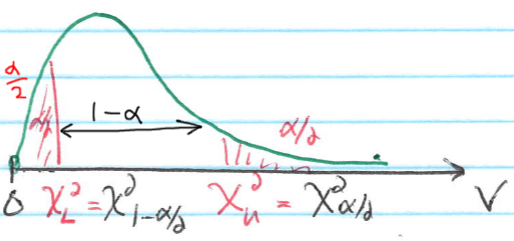
\includegraphics[width=3.5in]{89pic1.png}
\end{center}}
\noindent Then
\begin{align*}
	& \dfrac{\chi^2_L}{(n-1)S^2} \,\leq\, \dfrac{1}{\sigma^2} \,\leq\, \dfrac{\chi^2_U}{(n-1)S^2}\\\\
	\implies & \dfrac{1}{\chi^2_L} \,\geq\, \dfrac{\sigma^2}{(n-1)S^2} \,\geq\, \dfrac{1}{\chi^2_U}\\\\
	\implies & \dfrac{(n-1)S^2}{\chi^2_L} \,\geq\, \sigma^2 \,\geq\, \dfrac{(n-1)S^2}{\chi^2_U}\\\\
	\iff &  \color{red}\boxed{\color{black}  \dfrac{(n-1)S^2}{\chi^2_U} \,\leq\, \sigma^2 \,\leq\, \dfrac{(n-1)S^2}{\chi^2_L}}
\end{align*}
\begin{center}\red{Confidence interval for $\sigma^2$}\end{center}


\newpage
\addcontentsline{toc}{subsection}{Table 6: $\chi^2$ Lower Tail}
\notab{\begin{center} 
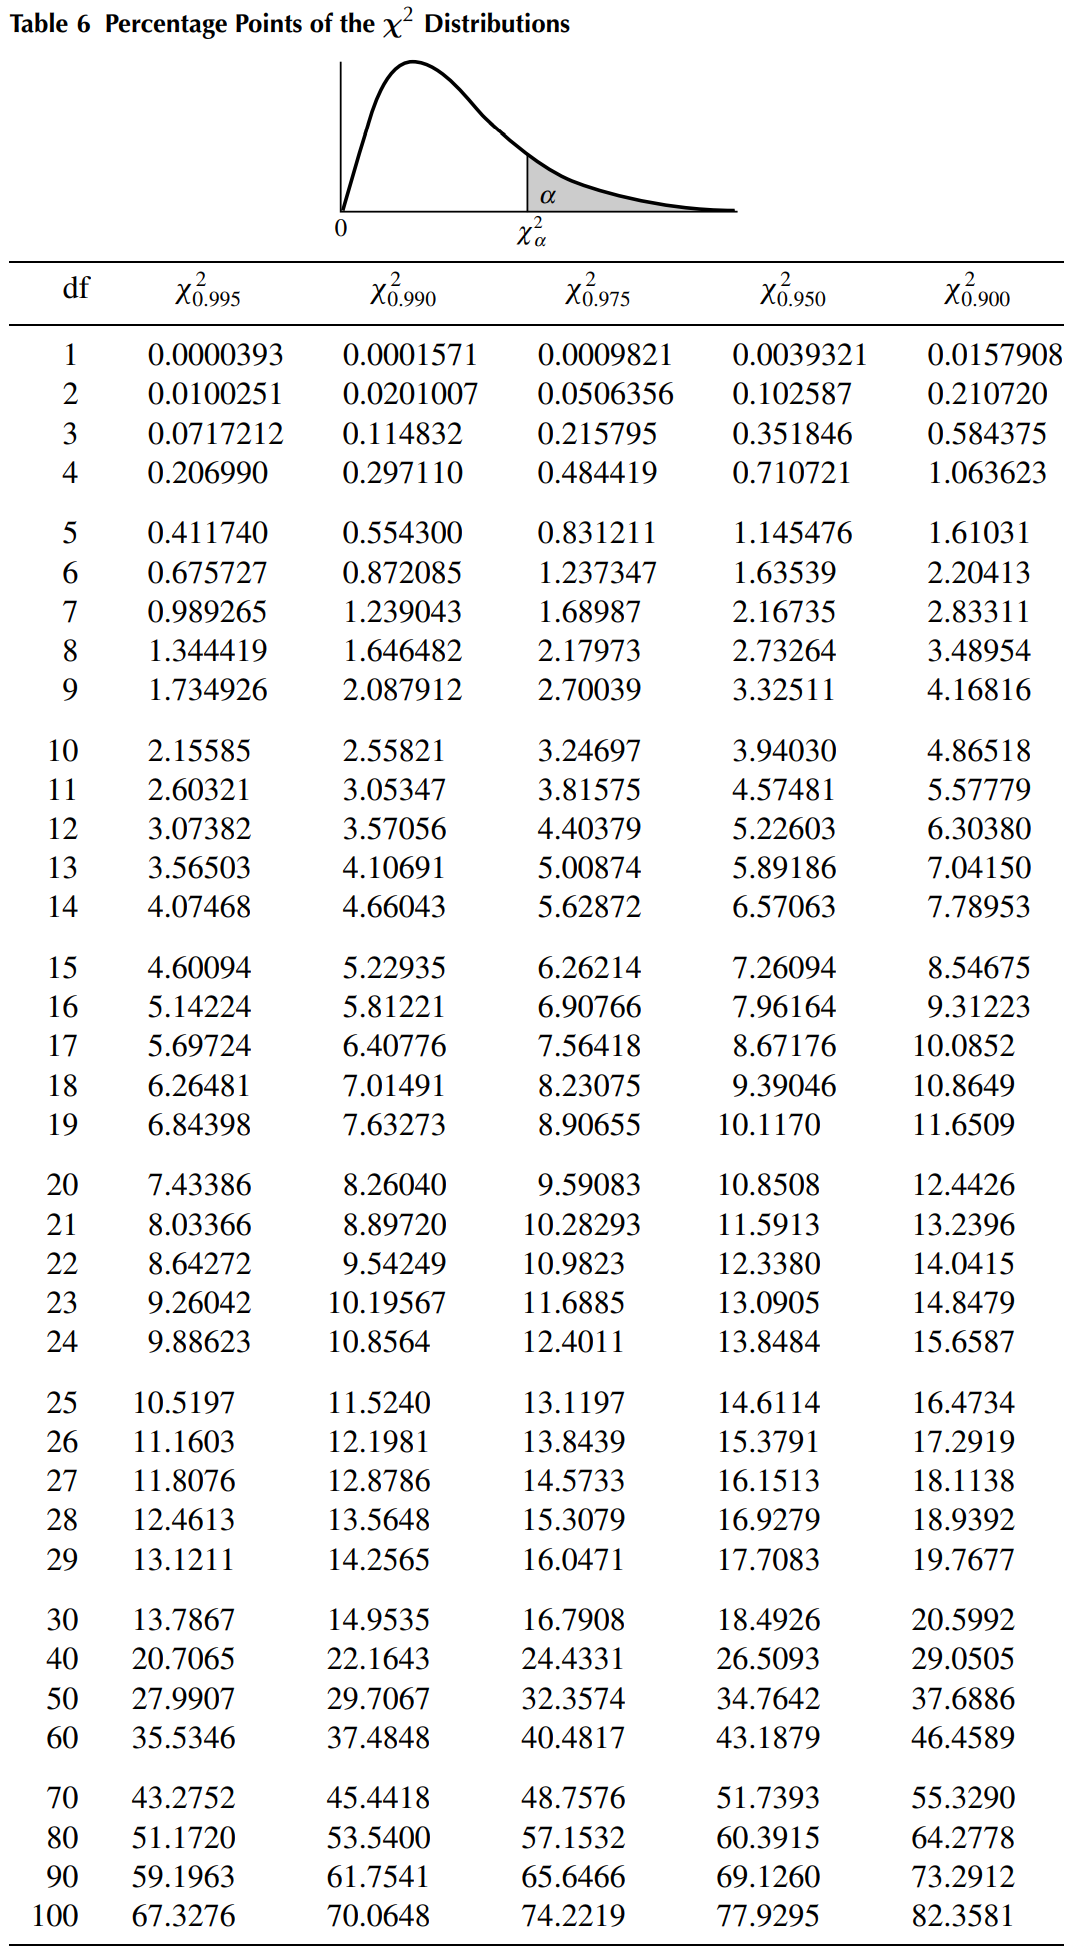
\includegraphics[width=5in]{Table6a.png}
\end{center}}

\newpage
\addcontentsline{toc}{subsection}{Table 6: $\chi^2$ Upper Tail}
\notab{\begin{center}
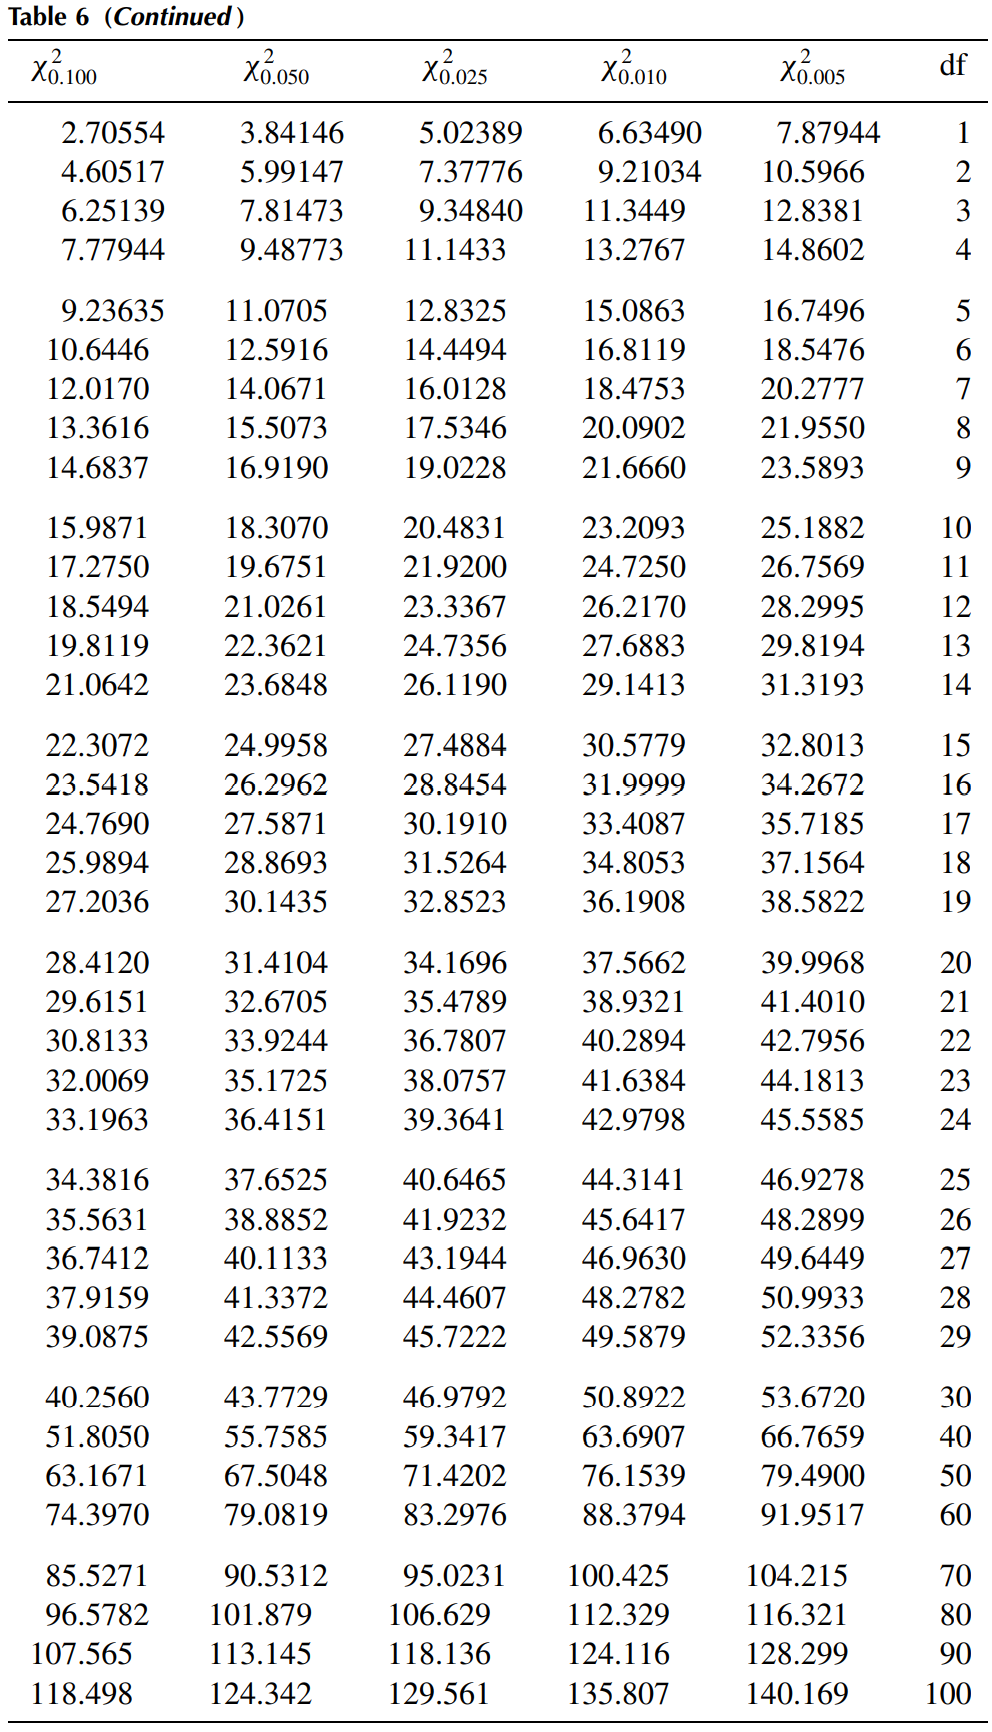
\includegraphics[width=5in]{Table6b.png}
\end{center}}

\newpage

\example Construct a 90\% C.I. for $\mu$ and $\sigma^2$.
$$\underbrace{85.4 \qquad 86.8 \qquad 86.1 \qquad 85.3 \qquad 84.8 \qquad 86.0}_{\textstyle \text{Data set, } n = 6}$$
$$\Xbar = 85.7\overline{3} \qquad S^2 = 0.502\overline{6} \qquad S \approx 0.7089$$
90\% C.I. $\implies \alpha = 0.10, \; \dfrac{\alpha}{2} = 0.05$ with df $n-1 = 5$.
$$\color{blue} \chi^2_L = \chi^2_{0.950} = 1.145476 \qquad \color{ggreen}\chi^2_U = \chi^2_{0.050} = 11.0705\color{black}$$

\nl A common mistake people make is forgetting that the lower bound is $\chi^2_U$. For $\sigma^2$,
\begin{center}
	$\dfrac{5\cdot(0.502\overline{6})}{\color{ggreen}11.0705}\color{black} \, \leq \, \sigma^2 \,\leq\, \dfrac{5\cdot(0.502\overline{6})}{\color{blue}1.145475\color{black}} $

	\nl $0.227 \,\leq\, \sigma^2 \,\leq\, 2.194$
	
	\nl $\sigma^2 \in (0.227,\;2.194)$\end{center}


\nl For $\mu$, use a $t$-distribution with 5 degrees of freedom.
$$\red{\Xbar} \pmp \color{ggreen}t_{0.050}\color{black} \cdot \color{blue}S\color{black}\quad\implies\quad \red{85.7\overline{3}} \pmp (\color{ggreen}2.015\color{black})(\color{blue}0.7089\color{black})$$
$$\mu \in (84.305,\; 87.162)$$
\chapter{Properties of Point Estimators and Methods of Estimation}
\setSection{1} \section{Relative Efficiency}
In general, given two estimators $\that_1$ and $\that_2$ of a parameter $\theta$, we claim the one with smaller MSE is better.

\nl For unbiased estimators, MSE \textit{is} variance $(\sigma^2)$. So an idea of \say{better} is if $\Var*{\that_1} < \Var*{\that_2}$, we say $\that_1$ is the better estimator.

\defn Given unbiased estimators $\that_1$ and $\that_2$ of $\theta$, the \bu{efficiency}of $\that_1$ relative to $\that_2$ is defined by
$$\eff*{\that_1,\; \that_2} = \dfrac{\Var*{\that_2} }{\Var*{\that_1} }.$$
\textit{Note: } If $\eff*{\that_1,\; \that_2} > 1$, then $\dfrac{\Var*{\that_2} }{\Var*{\that_1} } > 1 \implies \underbrace{\Var*{\that_1}  < \Var*{\that_2} }_{\textstyle \red{\that_1 \scriptstyle \text{ is \say{better}}}}$

\example Let $\thru{Y}$ be an iid random sample from $\normalDist*$. Two estimators of $\sigma^2$ are:
$$\widehat{\sigma^2_1} = S^2 = \dfrac{1}{n-1} \sum_{i=1}^n (Y_i -\Ybar)^2$$
$$\widehat{\sigma^2_2} = \over{2} \pars{Y_1 - Y_2}^2$$
We know $S^2$ is unbiased.

\newpage Show $\widehat{\sigma^2_2}$ is unbiased.
\begin{align*}
    \E*{\widehat{\sigma^2_2}} &= \E{\over{2}\pars{Y_1^2 - 2Y_1Y_2 + Y_2^2} }\\
    &= \over{2}\bigg[ \E{Y_1^2} -2\E{Y_1Y_2} + \E{Y_2^2} \bigg]\\
    &= \over{2}\bigg[ \Var{Y_1} + \big(\E{Y_1}\big)^2 -2\E{Y_1}\E{Y_2} + \Var{Y_2} +  \big(\E{Y_2}\big)^2 \bigg]\\
    &= \over{2}\bigg[ \sigma^2 + \mu^2 - 2\mu\cdot \mu + \sigma^2 + \mu^2 \bigg]\\
    &= \sigma^2 \qquad \text{\red{unbiased.}}
\end{align*}
To compute relative efficiency, we need variances.

\nl For $\Var{S^2}$, we know $\dfrac{(n-1)S^2}{\sigma^2} \sim \chi^2 (n-1)$.

\nl By properties of $\chi^2$ distribution, $\Var{\dfrac{(n-1)S^2}{\sigma^2}} = 2(n-1)$.

\nl Then, $\dfrac{(n-1)^2}{\sigma^4}\cdot \Var{S^2} = 2(n-1) \quad \implies \quad \Var{S^2} = \dfrac{2\sigma^4}{n-1}$.

\nnl For $\Var*{\widehat{\sigma^2_2}}$, this takes more work.
$$\Var{\over{2}(Y_1 - Y_2)^2} = \color{ggreen}\underbrace{\color{black}\E{\pars{\over{2}(Y_1 - Y_2)^2}^2}}_{\displaystyle \ast} \color{black} - \color{red}  \underbrace{\color{black}\brac{\E{\over{2}(Y_1 - Y_2)^2}}^2}_{\displaystyle \sigma^4}$$
\begin{align*}
    {\color{ggreen}\ast} &= \over{4} \E{(Y_1-Y_2)^4}\\
    &= \over{4} \E{Y_1^4   - 4Y_1^3Y_2    + 6Y_1^2Y_2^2    - 4 Y_1Y_2^3  + Y_2^4}\\
    &= \over{4} \biggbrac{\E{Y_1^4}  - 4\E{Y_1^3}\E{Y_2}  + 6\E{Y_1^2}\E{Y_2^2} - 4 \E{Y_1}\E{Y_2^3}  + \E{Y_2^4}}\\
    &= \over{4} \biggbrac{2\E{Y^4}  - 8\E{Y^3}\E{Y}  + 6\E{Y^2}^2}\\
\end{align*}
We need the higher moments $m_3'$ and $m_4'$. Recall the mgf for $\normalDist*$ is $m(t) = \exp \biggbrac{\mu t + \dfrac{t^2 \sigma^2}{2}}$

\nl 

\begin{align*}
    m'(t) &= (\mu + t \sigma^2)m(t)\\m'(0) &= \mu m(0) \\ &= \mu \\ &= \E{Y}\\\\
    m''(t) &= \sigma^2 m(t) + (\mu + t \sigma^2)^2 m(t)\\
    m''(0) &= \sigma^2 + \mu^2 m(0) \\ &= \sigma^2 + \mu^2 \\&= \E{Y^2}\\\\
    m^{(3)}(t) &= \sigma^2 m'(t) + 2(\mu + t \sigma^2) \sigma^2 m(t) + (\mu + t \sigma^2)^2 m'(t)\\
    m^{(3)}(0) &= \sigma^2 m'(0) + 2(\mu + 0 \sigma^2) \sigma^2 m(0) + (\mu + 0 \sigma^2)^2 m'(0)\\
    &= \sigma^2 \mu + 2\mu\sigma^2 + \mu^3\\
    &= \mu^3 + 3\mu\sigma^2\\
    &= \E{Y^3}\\\\
    m^{(4)}(t) &= \cdots \\
    m^{(4)}(0) &= \cdots \\
    &=  \mu^4 + 6\mu^2\sigma^2 + 3\sigma^4\\
    &= \E{Y^4}
\end{align*}
Substituting back into {\color{ggreen}*}, we get ${\color{ggreen}*} = \dfrac{1}{4} (12\sigma^4) = {\color{ggreen}3\sigma^4}$. Thus, 
$$\Var{\widehat{\sigma^2_2}} = \Var{\over{2}(Y_1 - Y_2)^2} = \color{ggreen}\underbrace{\color{black}3\sigma^4}_{\displaystyle \ast} \color{black} - \color{red}  \underbrace{\color{black} \sigma^4}_{\displaystyle \sigma^4}\color{black} = 2\sigma^4$$
Hence, $\eff*{S^2,\, \widehat{\sigma^2_2} } = \dfrac{\quad2\sigma^4\quad}{\frac{2\sigma^4}{n-1}} = n-1$
\newpage \section{Consistency}
\textbf{Discussion: } \say{Covergence in probability}

\nl This is a different type of analysis than that of Calculus.

\example MTH 420, \say{pointwise} convergence:
$$f_n(x) = x^n,\quad x \in [0,\,1] \qquad \limn f_n(x) = \begin{cases}0 & x \in [0,\,1)\\ 1 & x = 1\end{cases}$$

\nl Let $x \in (0,1)$. To show $x^n \to 0$:\\
For any $\epsilon > 0$, need an index $N$ such that when $n > N$ we get $\abs{x^n - 0} < \epsilon$
$$\text{Choose } \; N > \ceiling{\frac{\ln \epsilon}{\ln x}}$$
In probability, convergence is about the probabalistic measure of an event.

\example Law of Large Numbers:

\nl $A$, an event associated with an event $E$. $\Pr(A) = p.$

\nl Do $n$ iid repetitions of $E$ and count $n_A := \text{number of times } A \text{ occurs}$.

\nl The relative frequency $f_A = \dfrac{n_A}{n}$. \red{The Law of Large Numbers says $f_A \to p$}

\nl What does this mean exactly? \red{Conclusion: $\underbrace{\Pr(\abs{f_A-p}<\epsilon)}_{{\color{ggreen}*}} \geq 1 - \dfrac{p(1-p)}{n\epsilon^2}$}

\nl {\color{ggreen}*} This means the probability that $p$ is in the confidence interval $f_A - \epsilon \leq p \leq f_A + \epsilon$.

\nl Convergence? $\displaystyle \limn \Pr(\abs{f_A-p} < \epsilon ) \geq \limn \pars{1-\frac{p(1-p)}{n\epsilon^2}} = 1$
$$\implies \limn \Pr(\abs{f_A - p} < \epsilon) = 1$$
\begin{center}\red{This is convergence in probability!}\end{center}

\nl In probability, convergence is about the probabalistic measure of an event (measure theory).

\defn Estimatior $\that$ is \bu{consistent} if $\that \to \theta$ in probability.

\nl That is $\that_n$ is a consistent estimator of $\theta$ if for any $\epsilon > 0$
$$\limn \P{\abs{\that_n - \theta} \leq \epsilon} = 1$$

$$\text{or } \quad \limn \P{\abs{\that_n - \theta} > \epsilon} = 0$$

\disc A tool for showing consistency:

\nl \textbf{Theorem} \addcontentsline{toc}{subsection}{Consistency Theorem} An unbiased estimator $\that_n$ for $\theta$ is consistent if
$$\limn \Var*{\that_n} = 0$$

\begin{proof}
Let $\epsilon > 0$, then consider, 
$$\prob{\left| \that_n - \theta \right| > \epsilon}$$

\nl Recall Chebyshev's Theorem
$$\Pr (\abs{Y-\mu} > k\sigma) \leq \over{k^2}$$
Here $\epsilon = k\sigma_{\that_n} \implies k = \dfrac{\epsilon}{\sigma_{\that_n}}, \qquad \displaystyle 0 \leq \P{\left| \that_n - \theta \right| > \epsilon} \leq \frac{1}{(\epsilon \big/\sigma_{\that_n})^2}$

\nl Then
$$\P{\left|\that_n- \theta \right| > \epsilon} \leq \frac{\sigma_{\that_n}^2}{\epsilon^2} = \frac{\Var*{\that_n}}{\epsilon^2}$$

\nl As $n \to \infty$,
$$0 \leq \limn \P{\left| \that_n - \theta \right| > \epsilon} \leq \limn \frac{\Var*{\that_n}}{\epsilon^2} = 0$$
$$\implies \P{\left| \that_n - \theta \right| > \epsilon} = 0$$
Hence, $\that_n \to \theta$ in probability.
\end{proof}

\example (Common) Consistent Estimators

\begin{enumerate}[label=\textcircled{\raisebox{-1pt}{\arabic*}}]
	\item
		$\Ybar$ know unbiased for $\mu$ and
		$$\Var*{\Ybar} = \frac{\sigma^2}{n}$$
		Provided that $\sigma^2$ is finite, $\limn \Var*{\Ybar} = 0$

		\nl $\Ybar$ is consistant, that is, $\Ybar \to \mu$

	\item
		$\phat$ unbiased for $p$.
		$$\Var{\phat} = \frac{pq}{n} \quad \text{and}\quad \limn \Var{\phat} = 0$$
		$$\implies \phat \to p \text{ i.e. consistent}$$
\end{enumerate}

\nnl \textbf{Example: (9.17 \& 9.18)}\\$\thru{X}$ and $\thru{Y}$ are iid random samples with $\mu_x$ and $\mu_y$ \\but
$\Var*{X} = \Var*{Y} = \sigma^2$.

\begin{enumerate}[label=\textbf{\alph*}.) ]
	\item
		Show that $\Xbar - \Ybar$ is a consistent estimator of $\mu_x - \mu_y$.
		
		\nl \textbf{Solution:} We showed in Chapter 8 that $\E*{\Xbar - \Ybar} = \mu_x - \mu_y$ is unbiased.

		\nl Then $\Var*{\Xbar -\Ybar} = \Var*{\Xbar} + (-1)^2\Var{\Ybar} = \dfrac{2\sigma^2}{n}$.

		\nl Because $\displaystyle \limn \Var*{\Xbar -\Ybar} = 0$, we have consistency. 

	\item
		Show that the pooled estimator,
		$$S^2_p = \frac{\sum_1^n (X_i - \Xbar)^2 + \sum_1^n(Y_i - \Ybar)^2}{2n-2}$$
		is a consistent estimator of $\sigma^2$ when $X, Y \sim \normalDist*$.

		\nl \textbf{Solution:} To show unbiased we need $\Var{S_p^2}$.

		\nl \say{Trick,} convert to a distribution we understand well.
        \begin{align*}
		\underbrace{\frac{(2n-2)S_p^2}{\color{red}\sigma^2\color{black}}}_{\substack{\chi^2(2n-2)\\ \text{By Fisher's}} } &= \frac{\displaystyle \sum_{i=1}^n (X_i - \Xbar)^2 + \sum_{i=1}^n(Y_i - \Ybar)^2}{\color{red}\sigma^2\color{black}}\\
		&= \underbrace{\sum_{i=1}^n \pars{\frac{X_i - \Xbar}{\sigma}}^2 + \sum_{i=1}^n \pars{\frac{Y_i - \Ybar}{\sigma}}^2}_{\textstyle U_n \sim \chi^2 (2n-2)}
		\end{align*}

		$$\E{\frac{(2n-2)S_p^2}{\sigma^2}} = 2n-2 \text{ by properties of } \chi^2$$
		$$\frac{2n-2}{\sigma^2} \E{S_p^2} = 2n-2 \implies \E{S_p^2} = \sigma^2 \quad \text{\red{unbiased.}}$$
		
        \nnl For consistency, use same \say{trick.}
		$$\Var{\frac{(2n-2)S_p^2}{\sigma^2}} = \Var{U_n}$$
		$$\pars{\frac{2n-2}{\sigma^2}}^2 \Var{S_p^2} = 2\cdot(2n-2)\quad \text{ by properties of } \chi^2$$
		$$\Var{S_p^2} = \frac{2\sigma^4}{2n-2}$$
		$$\limn \Var{S_p^2} = 0 \;\text{ therefore } S_p^2 \text{ is consistent.}$$
\end{enumerate}

\newpage\noindent \textbf{Theorem:} \say{The Limit Laws} (For probability convergence)
\addcontentsline{toc}{subsection}{Probabalistic Convergence Limit Laws} 

\nl Let $\that_n \to \theta$ and $\Psihat_n \to \Psi$. Then,
\begin{enumerate}[label=\textcircled{\raisebox{-1pt}{\arabic*}}]
\item $\that_n + \Psihat_n \to \theta + \Psi$
\item $\that_n \cdot \Psihat_n \to \theta \cdot \Psi$
\item $\dfrac{\that_n}{\Psihat_n} \to \dfrac{\theta}{\Psi}$
\item If $g$ is a continuous function at $\theta$, then $g(\that_n) \to g(\theta)$
\end{enumerate}

\example $S_p^2$ again.
\begin{align}
    S^2_p &= \frac{\sum_1^n (X_i - \Xbar)^2 + \sum_1^n(Y_i - \Ybar)^2}{2n-2} \notag\\
    &=  \frac{(n-1)S_{\Xbar}^2 + (n-1)S_{\Ybar}^2}{2n-2}\notag\\
    &= \frac{S^2_{\Xbar} + S^2_{\Ybar}}{2}\notag
\end{align}

\nl But we already know $S_{\Xbar}^2 \to \sigma^2 \text{ and } S^2_{\Ybar} \to \sigma^2$

\nl Hence, by the Limit laws,
$$S_p^2 \to \frac{\sigma^2 + \sigma^2}{2} = \sigma^2$$

\disc Consistency and large $n$ confidence intervals

\nl We have $\Ybar_n \pm Z_{\alpha/2} \dfrac{S_n}{\sqrt{n}}$
By consistency, $\Ybar_n \to \mu$ and $S_n \to \sigma$

\nl Hence, when $\sigma$ is finite, $\Ybar_n \pm Z_{\alpha/2}\frac{S_n}{\sqrt{n}} \to \mu$

\nl Hence $\displaystyle \limn \Pr\pars{\abs{\Ybar_{(n)} - \mu < Z_{\alpha/2}\frac{S_n}{\sqrt{n}}} < \epsilon } = 1$

\nl That is, $\Ybar_{(n)} \pmp Z_{\alpha/2} \dfrac{S_n}{\sqrt{n}} \to\mu $ in probability.

\nl \say{Consistency justified our working assumption in Chapter 8}

\newpage \noindent \textbf{Example: (9.24)}

\nl Let $\thru{Z}$ be an iid random sample with $Z \sim N(0,1)$

\nl Let $\displaystyle U_n = \sum_{i=1}^n Z_i^2 \qquad Z = \frac{Z_i - \mu}{\sigma}$

\nl We \say{know} $U_n \sim \chi^2(n)$
$$\text{Showed in old HW that } Z^2 \sim X^2(n)$$

\nl In notes, we used the product of $n$ mgfs to show that $U_n \sim \chi^2(n).$

\nl Hence, $\E{U_n} = n$ and $\Var{U_n} = 2n$. Let
$$W_n := \over{n} U_n$$
Note that $\displaystyle \E{W_n} = \over{n}\E{U_n} = 1$

\nl \red{Hence, $W_n$ is an unbiased estimator when $\sigma^2 = 1$}
\begin{align*}
\Var{W_n} &= \Var{\over{n} U_n} \\
&= \over{n^2} \Var{U_n} \\
&= \over{n^2} \cdot 2n \\
&= \frac{2}{n}
\end{align*}

\nl Since $\displaystyle \limn \Var{W_n} = 0$, we get $W_n \to 1$ in probability.
\newpage \section{Sufficiency}
\disc Among a collection of estimators, how do we choose which one to work with and why?

\nl Conceptually: A statistic is deemed \bu{\color{neonorange}sufficient} if it \say{contains all of the available information about a parameter,} given some random sample.

\example

\nl Statistician 1 has the data $\thru{X}$ and computes an estimator $\that$.

\nl Statistician 2 has only the stat $T = \tau(\thru{X})$ estimating $\theta$.

\nl Sufficient implies both statisticians can make equally correct estimates about $\theta$. Equivalently, a sufficient estimator $\that$ utilizes all of the information in a sample relating to $\theta$.

\nl In either case, both are able to make the \say{same} conclusions about $\theta$. 

\defn Let $\yn$ be a sample from a probability distribution that is known up to parameter $\theta$.

\nl The statistic $T = \tau(\yn)$ is \bu{sufficient for $\theta$} if the conditional distribution of $\yn$ given $T$ does not depend on $\theta$.

\nnl \textit{Remark:} \bu{Sufficiency Principle:}

\nl Given 2 data sets $\thru{X}$ and $\thru{Y}$ where the stats $$\tau(\thru{X}) = \tau(\thru{Y}) = T$$
Any inference about $\theta$ should be the same regardless of the data set.

\example (One time only via the definition)

\nl Let $Y \sim \operatorname{Bern}(p)$\\
i.e. $\Pr(Y=1) = p,\; \Pr(Y=0) = 1-p$.

\nl Let $Y_n$ be a sequence of observations. We have $\phat = \dfrac{\sum Y_i}{n}$.

\nl \red{Sufficiency Principle:}

\nl Any sequence with $k$ 1's and $n-k$ 0's is going to yield the same $\phat$. In other words, same inferences about $p$.

\nl Let $S = \sum Y_i$

\nl To show $S$ is sufficient for $p$, we must show that the conditional distribution of the data $\yn$ given $S$ does not depend on $p$.

\newpage\noindent For $k \in (0, 1, 2, \dots, n), \; S = Y_1 + \cdots + Y_n = k$. We have,
\begin{align*}
    \prob{Y_1 = y_1, \dots,\; Y_n = y_n \mid S = k} &= \frac{\prob{Y_1 = y_1, \; \dots, \; Y_n = y_n \text{ and } S = k}}{\Pr(S=k)}\\
    &= \left\{ \begin{array}{cc}
        0 & \hspace{5mm} \sum Y_i \neq k \\
        \displaystyle \frac{\prob{Y_1 = y_2, \; \dots, \; Y_n = y_n \text{ and } S = k}}{\Pr(S=k)} & \hspace{5mm} \sum Y_i = k
        \end{array} \right.\\
     &=  \frac
     {\overbrace{\prod_{i=1}^n \Pr(Y_i=y_i)}^{\color{blue}\text{independent}}}
     {\underbrace{\Pr(S=k)}_
     {\color{red}\substack{\text{Binomial, } k \text{ \say{successes}}\\ \text{in } n \text{ trials}}
     \color{black}}}\\
     &= \frac
     {\displaystyle p^{y_1}(1-p)^{1-y_1} \times \cdots \times p^{y_n}(1-p)^{1-y_n}}
     {\displaystyle  \binom{n}{k}p^k (1-p)^{n-k}}\\\\
     &=  \frac
     {\displaystyle  p^{\textstyle \sum_1^n Y_i}(1-p)^{\textstyle n-\sum_1^n Y_i}}
     {\displaystyle  \binom{n}{k}p^k (1-p)^{n-k}}\\\\
     &= \frac
     {\displaystyle  p^k (1-p)^{n-k}}
     {\displaystyle \binom{n}{k}p^k(1-p)^{n-k}}\\\\
     &= \left\{ \begin{array}{cl}
        0 & \hspace{5mm} S \neq k \\\\
        \displaystyle \dfrac{1}{\displaystyle \binom{n}{k}} & \hspace{5mm} S = k  \qquad \leftarrow \text{ independent of } p
        \end{array} \right.
\end{align*}

\noindent \red{By definition, $S = \sum Y_i$ is sufficient.}

\nl \textit{Remark:} Started with $\phat = \frac{S}{n}$.

\nnl \textbf{Note:} Any one-to-one transformation (injection) of a sufficient stat will again be sufficient. 

\example $f(x) = \dfrac{x}{n}$ is an injection (has invertible form).

$$S \text{ sufficient} \implies \frac{S}{n} \text{ sufficient}$$
Thus $\phat$ is also sufficient.

\example $\sqrt{x}$ is also an injection on $[0,\,1]$.

\nl Thus $\sqrt{S}$ is sufficient.

\nnl \textbf{Topic:} The Factorization Theorem:

\nl \color{red}In practice we do not use the definition.\color{black}

\addcontentsline{toc}{subsection}{The Factorization Theorem}
\nl \textbf{Theorem: The Factorization Theorem}


\nl Let $\thru{X}$ denote a random sample from a distribution with pdf $f(x \mid \theta)$

\nl \color{orange}(distribution depends on the unknown parameter $\theta$)\color{black}

\nnl The statistic $T = \tau(\thru{x})$
is a sufficient statistic for $\theta$ if and only if the conditional pdf can be factored as follows.
$$L(\thru{x} \mid \theta) = g(\tau(\thru{x}) \mid \theta) \cdot h(\thru{x})$$
Where
\begin{itemize}
    \item $g$ is a function that depends on the data only through the stat $T$
    \item $h$ does not depend on $\theta$
\end{itemize}

\nnl\textit{Remarks:}
\begin{enumerate}[label=\textcircled{\raisebox{-1pt}{\arabic*}}]
    \item Via independence (of data)
    $$L(\thru{x} \mid \theta) = f(x_1 \mid \theta) \cdot f(x_2 \mid \theta) \times \cdots \times f(x_n \mid \theta)$$
    The product of the marginals.
    \vspace{.2in}
    \item The function $L$ is called the \bu{likelihood of the sample.}
\end{enumerate}

\example Let $\thru{X}$ denote a random sample from a Poisson distribution with parameter $\lambda > 0$. Find a sufficient statistic for the parameter $\lambda$.

\nl Here,
$$f(x) = \frac{\lambda^x e^{-\lambda}}{x!}\;,\; x = 0,\, 1,\, 2,\,\dots$$
\begin{align}
L(x_1,\, x_2\, \dots,\,x_m \mid \lambda) &= 
f(x_1 \mid \lambda)\cdot f(x_2 \mid \lambda)\times \cdots \times f(x_n \mid \lambda) \notag\\
&= \frac{\lambda^{x_1} e^{-\lambda}}{x_1!} \cdot \frac{\lambda^{x_2} e^{-\lambda}}{x_2!}\times \cdots \times \frac{\lambda^{x_n} e^{-\lambda}}{x_n!}\notag\\
&= \underbrace{\lambda^{x_1 + \cdots + x_n}e^{-\lambda n}}_{\substack{\color{ggreen}\textstyle S := \sum X_i\\ \color{ggreen}\textstyle g(S \mid \lambda) }} \cdot \underbrace{\frac{1}{x_1! \cdot x_2! \cdot \cdots \cdot x_n!}}_{\color{red}\textstyle h(\thru{x})}\notag
\end{align}
With $S=\sum X_i$,
$$\color{ggreen}g(S \mid \lambda)\color{black} = e^{-\lambda n}\lambda^S$$
and
$$\color{red}h(\thru{x})\color{black} = \over{x_1! \cdot x_2! \cdot \cdots \cdot x_n!}$$

\noindent \color{orange} By Factorization Theorem, $S$ is a sufficient statistic.\color{black}

\nnl \textbf{Note:} $\Xbar = \dfrac{1}{n} \sum X_i$ or $n\Xbar = S = \sum X_i$. So,
$$g(S \mid \lambda) = e^{-\lambda}\lambda^{n\Xbar} = g(\Xbar \mid \lambda)$$
Therefore $\Xbar$ is also a sufficient statistic.

\example The $\phat$ example again. $Y\sim \operatorname{Bern}(p)$.
\begin{align}
    L(\thru{y} \mid p) &= f(y_1 \mid p) \times \cdots \times f(y_n \mid p)     \notag\\
    &= p^{y_1}(1-p)^{1-y_1}\times \cdots \times p^{y_n}(1-p)^{1-y_n} \notag\\
    &= p^{\sum y_i}(1-p)^{n-\sum y_i} \hspace{0.5in} \color{orange}\textstyle S := \sum y_i\color{black} \notag\\
    &= \color{ggreen}\underbrace{\color{black} p^{\color{orange}S}(1-p)^{n-\color{orange}S}}_{\textstyle g(S \;\mid\; p)}\cdot \color{red} \underbrace{1}_{\textstyle h(\vec{y})} \notag
\end{align}
Where $\vec{y}$ is the $n$ tuple $y_1, y_2, \dots, y_n$.

\nl By Factorization Theorem, $S$ is sufficient.

\nnl \textbf{Yesterday:} Sufficiency
$\underbrace{f(\thru{x}\mid S)}_{S \text{ is sufficient for }\theta} = \underbrace{\frac{f(\thru{x} \text{ and } S(p) = s)}{f(s)}}_{\text{conditional prob is independent of } \theta}$

\nl Factorization theorem:
$$L(\thru{x} \mid \mu) = \underbrace{g(\mu,\;s)}_{\substack{S \text{ is} \\ \text{sufficient} \\ \text{for } \theta }} \cdot h(\vec{x})$$

\example Let $\thru{X}$ be a random sample from $N(\mu,1)$. \color{blue} (unknown $\mu$, $\sigma^2 = 1$.)\color{black}
$$f(x) = \frac{1}{\sqrt{2\pi} \exp\brac{\dfrac{-(x-\mu)^2}{2}}}$$

\nl Find a sufficient statistic for $\mu$.

\nl Construct Likelihood function,
\begin{align}
    L(\thru{x}\mid \mu) &= f(x_1 \mid \mu) \cdots f(x_n \mid \mu)\notag\\
    &= \frac{1}{\sqrt{2\pi}} \exp\brac{\frac{-(x_1-\mu)^2}{2}} \times \cdots\times \frac{1}{\sqrt{2\pi}} \exp\brac{\frac{-(x_n-\mu)^2}{2}}\notag\\
    &= \pars{\over{\sqrt{2\pi}}}^2\exp\brac{-\over{2} \sum (x_i - \mu)^2}\notag\\
    &= \over{(2\pi)^{n/2}}\exp\brac{-\over{2} \sum (x_i^2 - 2x_i\mu + \mu^2)}\notag\\
    &= \over{(2\pi)^{n/2}}\exp\brac{-\over{2} \sum (-2x_i\mu + \mu^2)}\cdot \exp\brac{-\over{2}\sum x_i^2}\notag\\
    &= \over{(2\pi)^{n/2}}\exp\brac{-\over{2}\pars{-2\mu \sum x_i + n\mu^2}}\cdot \exp\brac{-\over{2}\sum x_i^2}\notag\\
    &= \over{(2\pi)^{n/2}}\underbrace{\exp\brac{\mu \sum x_i -\over{2}n\mu^2}}_{\textstyle \text{Define } S := \sum x_i}\exp\brac{-\over{2}\sum x_i^2}\notag
\end{align}
\color{ggreen}
$$g(S \mid \mu) = \over{(2\pi)^{n/2}} \operatorname{exp}\brac{\mu S - \frac{n\mu^2}{2}}$$
\color{orange}
$$h(\vec{x}) = \operatorname{exp}\brac{-\over{2}\sum x_i^2}$$\color{black}
By Factorization Theorem, $S$ is a sufficient statistic for $\mu$.

\example (9.49)

\nl Suppose $X_i \sim \operatorname{Unif}(0,\,\theta)$, $\theta$ unknown. Then,
$$f(x) = \over{\theta} \,, \qquad x \in [0, \, \theta]$$
(In this, we use $X_{(n)} = \operatorname{max}\{\thru{x}\}$ as an estimator of $\theta$.)

\nl $f(x_1 \mid \theta) \times \cdots \times f(x_n \mid \theta) = \dfrac{1}{\theta^n}$
independent of any $x_i$'s.

\nl To bring the $x_i$'s into the story, we use the indicator function
$$I_{[0,\,\theta]}(x) = \begin{cases} 1 & x \in [0,\theta]\\ 0 & \text{else} \end{cases}$$
So, 
$$f(x) = \frac{I_{[0,\,\theta]}(x)}{\theta}$$
With this,
\begin{align}
    L(\thru{x} \mid \theta) &=  \frac{I_{[0,\,\theta]}(x_1)}{\theta} \times \cdots  \times \frac{I_{[0,\,\theta]}(x_n)}{\theta}\notag\\
    &= \over{\theta^n}I_{[0,\,\theta]}(x_i \in [0, \theta],\; i=1,2,\dots, n)\notag
\end{align}
Now, $x_i \leq \theta$ for all $i$ if and only if $\operatorname{max}\{\thru{x}\} \leq 0$. So,
$$L(\thru{x} \mid \theta) = \over{\theta^n}I_{[0,\,\theta]}(\operatorname{max}\{\thru{x} \leq \theta\})$$
Define statistic $T := \operatorname{max}\{\thru{x}\}$ and then
$$g(T \mid \theta) = \over{\theta^n}I_{[0,\,\theta]}(T)$$
$$h(\thru{x}) = 1$$
By the Factorization Theorem, $T = \operatorname{max}(\thru{x})$ is a sufficient statistic.

\nl \textbf{Note:} $\Xbar$ is not sufficient since there is no way to bring $\Xbar$ into $L$.\\
(Of course, no reason we should be able to do so since $\Xbar$ is also biased for $\theta\dots$ and clearly not consistent. $\Xbar \to \dfrac{\theta}{2}$ and these $\Xbar \to \theta$ in probability)
\newpage \section{Rao-Blackwell Theorem and Minimum-Variance Unbiased Estimation}%9.5
\textbf{Theorem: The Rao-Blackwell Theorem}

\nl Let $X$ and $Y$ be a random variable such that $\E{Y} = \mu$ and $\Var{Y} = \sigma^2 y.$

\nl Let $\phi(x) = \E{Y \mid X}$.

\nl Then $\E{\phi(x)} = \mu$ and $\sigma^2_{\phi(x)} \leq \sigma^2y$

\begin{proof}
    Have $f(x,y)$, $f_1(x)$, $f_2(y)$, and
    $$h(y\mid x) = \frac{f(x,y)}{f_1(x)} \color{red}{\ast}\color{black}$$
    
    \begin{align*}
        \phi(x) &= \E{\phi(x)} \\
        &= \int_{\R} yh(y \mid x)dy.\\
        &= \int_{\R} y\frac{f(x,y)}{f_1(x)}dy\\
        &= \over{f_1(x)}\int_{\R} yf(x,y) dy
    \end{align*}
    Then
    $$f_1(x) \phi(x) = \int_{\R} y f(x,y) dy$$
    \begin{align*}
        \E{\phi(x)} &= \int_{\R} \phi(x)f_1(x)dx\\
        &= \int_{\R} \brac{\int_{\R} y f(x,y) dy}dx\\
        &= \int_{\R}\int_{\R}f(x,y)dydx\\
        &= \int_{\R} y \brac{\int_{\R}f(x,y)dx}dy\\
        &= \int_{\R} y f_2(y)dy \\
        &= \E{Y} \\
        &= \mu.
    \end{align*}

\nl Note that $\sigma^2_{\phi(x)} = \E{(\phi(x)-\mu)^2}.$
\begin{align*}
    \sigma_y^2 &= \E{(y-\mu)^2}\\
    &= \E{(\color{red}(\color{black}y \color{orange}-\phi(x) \color{red})(\color{orange}\phi(x)\color{black}-\mu \color{red})\color{black}  ^2}\\
    &=\E{ (y-\phi(x))^2 + 2(y-\phi(x))(\phi(x)-\mu) + (\phi(x)-\mu)^2}\\
    &= \underbrace{\E{(y-\phi(x))^2}}_{\textstyle \geq\; 0} + \underbrace{2\E{(y-\phi(x))(\phi(x)-\mu)}}_{\textstyle \color{orange}\ast\color{black}} + \underbrace{\E{(\phi-\mu)^2}}_{\textstyle \color{red}\sigma^2_{\phi(x)}\color{black}}\\
    \color{orange}(\ast) \color{black} &= \int_{\R} \int_{\R} (y-\phi(x))(\phi(x)-\mu)f(x,y)\,dydx\\
    &= \int_{\R}(\phi(x)-\mu)\brac{\int_{\R}(y-\phi(x))f(x,y)\,dy}dx\\
    \color{red}(\ast) \color{black} &= \int_{\R} (\phi(x)-\mu)\brac{\int_{\R} (y-\phi(x)) f_1(x) h(y \mid x) \,dy }dx\\
    &= \int_{\R} (\phi(x)-\mu)f_1(x)\brac{\underbrace{\int_{\R} (y-\phi(x))h(y\mid x)\,dy}_{\text{\color{orange}note**\color{black}}}}dx\\
    &= 0
\end{align*}
\color{orange}\textbf{Note**}: This is \underline{zero} as $$\phi = \E{y \mid x} = \int yh(y\mid x)\,dy$$\color{black}

\nl So $\sigma^2_y = \E{(y-\phi(x))^2}+\sigma^2_{\phi(x)} \geq \sigma^2_{\sigma(x)}$

\nl Aside: This almost always a strict inequality. For equality,
$$\P{Y-\phi = 0} = 0$$
\end{proof}

\disc Using the RBT (Rao-Blackwell Theorem) to construct \say{best} statistics.

\nl Big Idea: We can take any unbiased estimator of $\theta$ and combine with a sufficient stat for $\theta$ to get a \say{better} estimator.

\nl Let $\thru{x}$ denote a random sample of $f(x \mid \theta)$. We have $T = \tau(\thru{x})$ sufficient for $\theta.$ Let $U = u(\thru{x})$ be an unbiased stat for $\theta$ which is not itself a function of $T$. Consider $\E{u \mid T}$:

\noindent Since $T$ is sufficient, the conditional probability of $U$ given $T = \tau$ does \underline{not} depend upon $\theta$.

\nl Define a new stat
$$\phi(\tau) = \E{U \mid T}$$
which is a function of $\tau$ alone. Hence, $\phi(T)$ is a statistic (does not depend opon $\theta$). (i.e. only a function of the data.)

\nl By RBT, $\phi(T)$ is an unbiased statistic for $\theta$ with the guarantee that
$$\sigma^2_{\phi(T)} < \sigma^2_u$$

\nnl Theorem: Rao-Blackwell Theorem (Textbook version):

\noindent Let $\that$ be an unbiased estimator for $\theta$ such that $\Var*{\that} < \infty$.\\If $T$ is a sufficient statistic for $\theta$, define $\that^* = \E{\that^* \mid T}$.

\nl Then, for all $\theta$, $\E{\that^*}= \theta$ and
$$\Var*{\that^*} \leq \Var*{\that}$$

\disc Minimum Variance Unbiased Estimator (MVUE)

\nl If $\that$ is an MVUE, then
$$\Var*{\that} \leq \Var*{\Psihat} \quad \text{for any other estimator } \Psihat.$$

\nl \underline{Typically} (almost always) the process we described above lends to an MVUE.

\begin{enumerate}[label=\textcircled{\raisebox{-1pt}{\arabic*}}]
    \item $\that$ unbiased estimator for $\theta$
    \item $T$ sufficient for $\theta$
    \item $\E{\that \mid T}$ is a MVUE
\end{enumerate}

\nl Remark: All of yesterdays sufficiency examples indicate that all traditional estimators are MVUE.

\example $\operatorname{Bern}(p)$\\
Here unbiased estimator $\phat = \dfrac{S}{n}$.\\
Here $S = \sum Y_i$ is sufficient.
$$\E{\phat\mid S} = \frac{S}{n} \text{ sufficient stat, has no } p.$$
Rao-Blackwell $\quad \implies \quad \phat \text{ is an}$ MVUE.

\nl Also note, $\Var{\phat} < \Var{S}$, is much better $\dfrac{p}{n} < np$.

\example Last day we showd that $S = \sum Y_i$ is a sufficient stat for $\lambda$ in $\operatorname{Pois}(\lambda)$.
$$f(y) = \frac{\lambda^ye^{\lambda}}{y!}\;, \quad y = 0, 1, 2, \dots$$

\nl We seek an MVUE of $e^{-\lambda}$. Need an unbiased estimator of $\thru{Y}$ iid.

\begin{enumerate}[label={\alph*})]
    \item Show that
    $$W= \begin{cases} 1 & Y_1 = 0\\0 & Y_1 \neq 0\end{cases}$$
    is unbiased for $e^{-\lambda}$. (New idea: Not just looking for $\lambda$, but a function of $\lambda$.)
    
    %add align
    \nl \textbf{Solution:} $\E{W} = 1 \cdot \P{Y_1 = 0} + 0 \cdot \P{Y_1 \neq 0} = \P{Y_1 = 0} = \dfrac{\lambda^0 e^{-\lambda}}{0!} = e^{-\lambda}$

    \item Use RBT to find a MVUE. Compute $\E{W \mid S}$
    \begin{align}
        \E{W \mid S} &= 1 \cdot \Pr(Y_1 = 0 \mid Y_1 + Y_2 + \cdots + Y_n = S) + 0 \cdot \Pr(Y_1 \neq 0 \mid S)\notag\\
        &=\frac
        {\Pr(Y_1 = 0 \;\text{ and }\; \sumThru{Y} = S)}
        {\Pr(\sumThru{Y} = S)}\notag\\
        &= \frac
        {\Pr(Y_1 = 0 \;\text{ and }\; Y_2 + \cdots + Y_n = S)}
        {\Pr(\sumThru{Y} = S)}\quad \text{top now independent events}\notag\\
        &= \frac{\Pr(Y_1=0)\cdot \Pr(Y_2 + \cdots + Y_n = S)}{\Pr(\sumThru{Y} = S)}\notag\\
        &= \frac{ e^{-\lambda} \cdot \Pr(Y_2 + \cdots Y_n = s)}{\Pr(Y_1 + \cdots + Y_n = s)}\notag
    \end{align}
    \color{red}325 FACT: \color{black} How is $Y_1 + \cdots + Y_n$ distributed? $Y_i \sim \operatorname{Pois}(\lambda)$.
    
    \nl Via moment generating functions, we proved that $Y_1 + \cdots + Y_n \sim \operatorname{Pois}(n\lambda)$

    \nl Hence $Y_2 + \cdots + Y_n \sim \operatorname{Pois}\pars{(n-1)\lambda}$, so
    \begin{align}
        \E{W \mid S} &=
        \frac{e^{-\lambda}\pars{\dfrac{((n-1)\lambda)^S e^{-(n-1)\lambda} }{S!} } }
        {\dfrac{(n\lambda)^S e^{-n\lambda}}{S!} } \notag\\
        &= e^{-\lambda} \pars{\frac{(n-1)\lambda}{n\lambda}}^S\cdot \frac{e^{-(n-1)\lambda}}{e^{-n\lambda}} \notag\\
        &= e^{-\lambda} \cdot \pars{\frac{n-1}{n}}^S e^{\lambda}\notag\\
        &=  \pars{\frac{n-1}{n}}^S\notag
    \end{align}
    By RBT, $\displaystyle \phi(S) =  \pars{\frac{n-1}{n}}^S$ is an MVUE of $e^{-\lambda}$, $\displaystyle S = \sum Y_i$.

    \nnl Aside: $$e^{-\lambda} = \limn \pars{1-\over{n}}^n$$
    $$\phi(S) =  \limn \pars{1-\over{n}}^S$$
\end{enumerate}
\newpage \section{The Method of Moments}%9.6
This is out oldest estimation technique. If there are $k$ parameters that have to be estimated, set the $1^{\text{st}}$ $k$ population moments \underline{(given in terms of the parameters)} and set them equal to the sample moments.

\recall*
$$\underbrace{\mu_k' = \E{Y^k}}_{\textstyle \text{\color{red}population}} \qquad \text{and} \qquad \underbrace{m_k' = \over{n}\sum Y_i^k}_{\textstyle \text{\color{red}data set}}$$

\example Let $Y \sim \normalDist*$. Then
\begin{align*}
\mu_1' &= \E{Y} = \mu\\
\mu_2' &= \E{Y^2} = \sigma^2 + \mu^2\\\\
m_1' &= \over{n}\sum Y_i = \Ybar\\
m_2' &= \over{n}\sum Y_i^2
\end{align*}
Set equal and solve for paramters, then 
$$\mu = \Ybar$$
$$\sigma^2 + \mu^2 = \over{n}\sum Y_i^2$$
Want $\sigma^2$ in terms of sample moments.
$$\sigma^2 + \Ybar ^2 = \over{n}\sum Y_i^2$$
$$\sigma^2 = \over{n}\sum Y_i^2 - (\Ybar)^2$$
Yields 2 estimators:
\begin{align*}
    \that &= \Ybar \quad \text{for } \mu\\
    \Psihat &= \over{n} \sum Y_i^2 - (\Ybar)^2 \quad \text{for } \sigma^2
\end{align*}
Note: $\Psihat$ is our \say{old} biased estimator for $\sigma^2$. While both of these are consistent stats, $\Psihat$ is biased as $\E*{\Psihat} = \dfrac{n-1}{n}\sigma^2$.

\example Suppose $\thru{Y} \sim \gammaDist{\alpha}{\beta}$. Use MoM to find estimators for $\alpha$ and $\beta$.

\nnl Recall for Gamma, $\E{Y} = \alpha\beta$, $\Var{Y} = \alpha\beta^2$. So,

\begin{align*}
    \mu_1' &= \alpha\beta\\
    m_1' &= \Ybar\\
    \mu_2' &= \over{n}\sum Y_1^2\\
    &= \E{Y^2} \\
    &= \Var{Y} + \pars{\E{Y}}^2\\
    &= \alpha\beta^2 + (\alpha\beta)^2\\
    &= \beta^2(\alpha + \alpha^2)\\
    m_2' &= \over{n}\sum Y_i^2
\end{align*}

\nl \red{System:} $\qquad \alpha\beta = \Ybar \qquad  \beta^2(\alpha + \alpha^2) = m_2' \qquad \alpha = \dfrac{\Ybar}{\beta} \qquad$ Then,
\begin{align}
m_2' &= \beta^2 \pars{\frac{\Ybar}{\beta} + \frac{\Ybar^2}{\beta^2}}\notag\\
&= \Ybar^2 + \beta \Ybar \notag\\
\Longleftrightarrow \quad \beta\Ybar &= m_2' - \Ybar^2 \notag\\
\Longleftrightarrow \quad \beta &= \frac{m_2' -\Ybar^2}{\Ybar}\notag\\
\Longrightarrow \quad \alpha &= \frac{\Ybar^2}{m_2'-\Ybar^2}\notag
\end{align}

\nl Define $\alpha$'s estimator $\displaystyle \that :=  \frac{\Ybar^2}{m_2'-\Ybar^2}$.

\nl and $\beta$'s estimator $\Psihat := \dfrac{m_2' -\Ybar^2}{\Ybar}$.

%new day
\nnl The following is the last example using MoM:

\example* $\thru{Y} \sim \operatorname{Unif}(0,\,\theta)$, with $\theta$ unknown.

$$\mu_1' = \E{Y} = \frac{\theta}{2} \hspace{1in} m_1' = \over{n} \sum Y_i = \Ybar$$
Mom set equal solution for population parameters.
$$\frac{\theta}{2} = \Ybar \quad \Longrightarrow \quad \theta = 2\Ybar$$
Define $\that := 2\Ybar$.

\nl So this is another estimator for $\theta$. Is it any good?

\nl Well, it is unbiased since $\E{2\Ybar} = 2\cdot\frac{\theta}{2} = \theta$ and it is consistent.

\nl Use variance trick to show$\dots$

$$\Var{2\Ybar} = 4\Var{\Ybar} = 4 \frac{\Var{Y}}{n} = 4 \cdot \frac{\theta^2 / 12}{n} = \frac{\theta^2}{3n}$$

\nl Note:
$$\limn \Var{2\Ybar} = \limn \frac{\theta^2}{3n} = 0$$
Consistent by theorem. However, earlier we showed $\Psihat = \max{\thru{Y}}$ is sufficient. Consider $\Var*{\Psihat}$.

\nl Like in Homework, $\displaystyle F(y) = \int_0^y \frac{1}{\theta}\,dy = \frac{y}{\theta}$
$$\P{Y_{(n)} \leq y} = \pars{\frac{y}{\theta}}^n = \frac{y^n}{\theta^n}.$$

\nl And $\displaystyle f_{(n)}(y) = \frac{ny^{n-1}}{\theta^n}$, thus
$$\E*{\Psihat} = \int_0^{\theta} y \cdot f_{(n)}(y)\,dy = \frac{n}{n+1}\theta.$$
$\Psihat$ is biased but it is consistent since $\displaystyle \limn \operatorname{E}[\,\Psihat\,] \to \theta$. For $\Var*{\Psihat} = \E*{\Psihat^2} - \E*{\Psihat}^2$:
$$\E*{\Psihat^2} = \int_0^{\theta} y^2 \cdot \frac{ny^{n-1}}{\theta^n} = \frac{n}{n+2}\theta^2$$
So...
$$\Var*{\Psihat} =  \frac{n}{n+2}\theta^2 - \pars{\frac{n}{n+1}\theta}^2 = \frac{n\theta^2}{(n+1)^2(n+2)}$$
And this variance is much better than $\Var*{\that}$.

$$\bias*{\that} = 0$$
$$\bias*{\Psihat} = \frac{n}{n+1} \theta - \theta = -\frac{\theta}{n+1}$$%the RH value is wrong
$$\MSE*{\that} = \Var{\that} + \bias*{\that}^2 = \frac{\theta^2}{3n}$$
$$\MSE*{\Psihat} = \frac{n\theta^2}{(n-2)(n+1)^2} + \frac{\theta^2}{(n+1)^2}$$
We see both $\Var*{\Psihat} < \Var*{\that}$ and $\MSE*{\Psihat} < \MSE*{\that}$

\nl Of course, if we were to define
$$\Psitil := \frac{n+1}{n}\Psihat$$
Now we have an unbiased consistent statistic. Last day, we showed that $\Psihat$ is sufficient. So by the Rao-Blackwell Theorem, $\Psitil$ will be an MVUE. That is, $\Var*{\Psitil} \leq \Var*{\Psihat}$.

\newpage \section{The Method of Maximum Likelihood}%9.7
Recall, the likelihood function is simply the joint pdf with the interpretation that a parameter(s) is unknown.
$$Y_1 \sim \text{ via } f(y \mid \theta)$$
$Y_i$'s are iid random sample.

\nl If $\theta$ is known, the joint pdf is
\begin{align}
    \setGreen \underbrace{\setBlack f(\thru{y})}_{\text{domain } f\; \subseteq\; \R^n}\setBlack  &= \color{red} \underbrace{\setBlack f_1(y_1) \cdot f_2(y_2) \cdots f_n(y_n)}_{\text{product of marginals}} & \text{ by independence}\notag\\
    &= f(y_1) \cdot f(y_2) \cdots f(y_n) & \text{by i.i.d.}\notag\\
    &= \prod_{i=1}^n f(y_i)\notag
\end{align}
If $\theta$ unknown, we emphasize this via the \bu{likelihood function}.
%make left underbrace green, right red
$$\setGreen \underbrace{ \setBlack L(\thru{Y} \mid \theta) }_{\text{domain } L\; \subseteq\; \R^{n+1}} \setBlack = \color{red} \underbrace{\setBlack f(y_1 \mid \theta) \cdot f(y_2 \mid \theta) \times \cdots\times f(y_n \mid \theta)}_{\text{really the same}}$$

\disc The reason this is called a \say{likelihood} function. Given a set of observations $Y_i$, what is the most likely value of $\theta$. 

\nl \underline{Fix} $(\thru{Y})$, $L$ at this number is a 1 variable function in terms of $\theta$.
\begin{center}
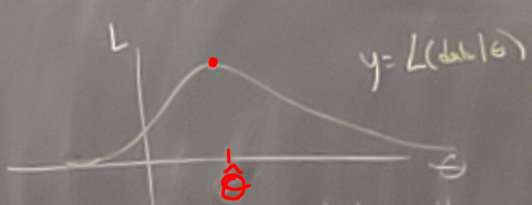
\includegraphics[width=4in]{L fn.png}
\end{center}
\nl Given this data set, what is the most likely value that $\theta$ takes? That would be $\theta$ corresponding to the largest value of pdf $\prod_i^n f(y_i \mid \theta)$.

\nl How do we find the largest? (\color{red}Optimize with respect to $\theta$\color{black}). That is, set $\displaystyle \pdv{L}{\theta} = 0$ solve and verify.

\defn The solution to $L_{\theta} = 0$ defines an estimator $\that$ of $\theta$, called the maximum likelihood estimator (MLE).

\nl \textit{Remark:} In computations, verify the critical point \textit{is} a maximum.

\newpage\noindent\example* $X \sim \operatorname{Bern}(p) = \operatorname{Binom}(1,p)$

\nl Given $\thru{X}$ an iid sample.
\begin{align}
    L(\thru{X} \mid p) &= p^{X_1}(1-p)^{1-X_1} \cdots p^{X_n}(1-p)^{1-X_n} \notag\\
    &= p^S(1-p)^{n-S}, \qquad S := \sum X_i\notag
\end{align}
Then,
\begin{align}
    \pdv{L}{p} &= Sp^{S-1}(1-p)^{n-S} + p^S (n-s)(1-p)^{n-S-1} (-1)\notag\\
    &= p^{S-1}(1-p)^{n-S-1}\brac{S(1-p)-p(n-S)}\notag
\end{align}
And $\displaystyle \pdv{L}{p} = 0$ when 
\begin{align}
    S - Sp - pn + Sp &= 0\notag\\
    S-pn &= 0\notag\\
    p &= \frac{S}{n} = \Xbar\notag
\end{align}
Is this a max? Yes, use the $1^{\text{st}}$ derivitive test: $\displaystyle \pdv{L}{p} = p^{S-1}(1-p)^{n-S-1} \brac{S-pn}.$

\nl If $p < \dfrac{S}{n}$, then $\;\displaystyle \pdv{L}{p} > 0.\;$

\nl If $p > \dfrac{S}{n}$, then $\;\displaystyle \pdv{L}{p} < 0$

\nl Therefore $\Xbar$ is an MLE for $p$. 

\disc The log-likelihood function.
$$L(\vec{X} \mid \theta) = \prod_{i=1}^n f(X_i \mid \theta)$$
Always an $n$-product. Depending on $f$, computing $\pdv{L}{\theta}$ can be difficult.

\nl Since $f(X_i \mid \theta) > 0$ and we have a function whose existance is to turn products into sums$\dots$

\defn The log-likelihood function:
$$\ln L(\vec{X} \mid \theta)$$
Claim: The MLE of $L(\vec{X} \mid \theta)$ also maximizes $\ln L(\vec{X} \mid \theta)$

\nl Reason:
$$\pdv{}{\theta}\pars{\ln L(\vec{X} \mid \theta)} = \frac{\displaystyle \pdv{L}{\theta} \pars{\vec{X}\mid \theta}}{L(\vec{X} \mid \theta)} = 0 \quad \iff \quad \; \pdv{}{\theta}\pars{L(\vec{X} \mid \theta)} = 0$$

\example The last one again\dots
$$L(\thru{X}\mid p) = p^S (1-p)^{n-S}, \quad S := \sum X_i$$
$$\ln L(\vec{x} \mid p) = S\ln p + (n-S)\ln (1-p)$$
$$\pdv{}{p}\pars{\ln L} = \frac{S}{p} + (n-s) \cdot \frac{-1}{1-p}$$
\begin{align}
    \pdv{}{p}\pars{\ln L} = 0 \quad \Longleftrightarrow& \quad S(1-p) + (n-S)(-p) = 0\notag\\
    \Longleftrightarrow& \quad S - Sp - np + Sp = 0\notag\\
    \Longleftrightarrow& \quad p = \frac{S}{n}\notag
\end{align}

\nnl \textbf{Topic: } More population parameters.

\nl This idea scales. If $f$ depends upon $k$ unknowns $\theta_1, \dots, \theta_k$, then define
$$L(\thru{X} \mid \theta_1, \dots, \theta_k) = \prod_{i=1}^n f(x_i \mid \theta_1, \dots, \theta_k)$$
Optimizing this is a calculus problem.

\remark* We could have also extended the idea of the Factorization Theorem the same way with sufficient statistics to get 
$$L(\thru{x} \mid \theta_1, \dots, \theta_k) = \blue{g(S_1, \dots, S_k, \theta_1, \dots, \theta_k) }\cdot \red{h(\thru{x})}$$

\example* Let $\thru{X}$ be an iid from $\normalDist*$ with both parameters unknown. Find the MLE for $\mu$ and $\sigma^2$.

\nl For ease of computation, $N(\mu, \theta)$ such that $\theta := \sigma^2$.
$$L(\thru{x} \mid \mu_1 = \theta) = \prod_{i=1}^n \over{\sqrt{2\pi\theta}}\exp\brac{-\dfrac{(X_i-\mu)^2}{2\theta}}$$
Fixing $\vec{x}$, we consider $L_{\vec{x}}(\mu,\;\theta)$\dots. I have no intentions of $\nabla L_{\vec{x}}$ under a product sign\dots
\begin{align*}
    \ln L &= \sum_{i=1}^n \pars{\ln(\over{\sqrt{2\pi\theta}}) + \dfrac{-(X_i-\mu)^2}{2\theta}}\\
    &= - \over{2} \ln (2\pi\theta)n - \over{2\theta} \sum_{i=1}^n (X_i-\mu)^2
\end{align*}
\begin{align*}
    \pdv{}{\mu}\pars{\ln L} &= 0 - \over{2\theta} \sum_{i=1}^n 2(X_i-\mu)(-1)\\
    &= \over{\theta} \sum (X_i-\mu)\\
    &= 0 \quad \text{when} \quad \textstyle \sum X_i - n\mu = 0 \rightarrow \widehat{\mu} = \Xbar 
\end{align*}
$$\text{i.e. } \mu = \dfrac{1}{n}\sum X_i = \Xbar$$

\begin{align*}
    \pdv{}{\theta}\pars{\ln L} &= -\frac{n}{2} \cdot \frac{2\pi}{2\pi\theta} + \over{2\theta^2} \sum_{i=1}^n(X_i-\mu)^2\\
    &= -\frac{n}{2\theta} + \over{2\theta^2} \sum_{i=1}^n(X_i-\mu)^2\\
    &= 0 \quad \text{At our potential critical point } \mu = \Xbar\\
    &\iff -n\theta + \sum_{i=1}^n(X_i-\Xbar)^2 = 0\\
    \text{or } & \that = \over{n}\sum_{i=1}^n(X_i-\Xbar)^2\\
    & \red{\text{our old biased estimator for } \sigma^2}
\end{align*}
Is this a max? We need to construct the Hessian Matrix\dots
\begin{align*}
    H &= \bmat{\ln L_{\mu\mu}}{\ln L_{\mu\theta}}{\ln L_{\theta\mu}}{\ln L_{\theta\theta}}\\
    &= \bmat{-\dfrac{n}{\that}}{-\dfrac{\sum X_i - n\mu }{\that^2}}{-\dfrac{\sum X_i - n\mu }{\that^2}}{\dfrac{n}{2\that^2}-\dfrac{1}{\that^3} \sum(X_i-\mu)^2}\\
    \text{At } (\widehat{\mu},\;\that) \\
    H(\mu, \theta) &= \bmat{-\dfrac{n}{\that}}{0}{0}{\dfrac{n}{2\that^2}-\dfrac{1}{\that^3} \sum(X_i-\mu)^2}
\end{align*}
For a maximum, by the $2^{\text{nd}}$ derivitive test, we need $(\ln L)_{\mu\mu} = -\dfrac{n}{\that} < 0$, \hspace{.1cm} \red{which it is! } And $\det H > 0$.

\nl Note, $\displaystyle (\ln L)_{\theta\theta} = \dfrac{\that n - 2 \sum(X_i - \Xbar)^2}{2 \that^3}$.

\nl But $n\that = \sum (X_i - \Xbar)^2$, so $\displaystyle (\ln L)_{\theta\theta} = \dfrac{\that n - 2 \that n}{2 \that^3} = - \frac{n}{2\that^2} \;\red{ < 0}$.

\nl So $\displaystyle \det H = \dfrac{-n}{\that} \cdot \dfrac{-n}{2\that^2} = \dfrac{n^2}{2\that^3}\;\red{ > 0 }$. Hence $(\Xbar,\, \that)$ is the location of a MLE by the 2nd derivitive test.

\disc Why MLEs? Because they have nice properties.
\begin{enumerate}[label=\textcircled{\raisebox{-1pt}{\arabic*}}]
    \item If $U$ is a sufficient statistic of $\theta$, then the MLE \red{is} a function of $U$.
    
    \nl Reason: If $U$ is sufficient, then $L(\vec{x} \mid \theta)$ is factorable:
    $$L(\thru{x} \mid \theta_1, \dots, \theta_k) = g(U, \theta) \cdot h(\thru{x})$$
    This $\displaystyle \pdv{L}{\theta} = \pdv{g}{\theta} \cdot h(\vec{x})$ 
    $$\text{i.e. }\; \underbrace{ \pdv{L}{\theta} = 0 }_{  
        \substack{ \text{sol'n to this is} \\ \that \text{ (the MLE)} }
    } \iff \underbrace{\pdv{g}{\theta} = 0}_{
        \substack{\text{sol'n to this is} \\ \that \text{ a function of } U}
    }$$

    \item The invariance properties of the MLE.
    
    \nl Suppose we want to estimate a function of the parameter (say $t(\theta)$). If $t$ is a one-to-one (injective) function (i.e. invertible), the MLE of $t(\theta)$ will be simply $t(\that)$, where $\that$ is the MLE of $\theta$.

    \nl Reason: Let $t(\theta)$ be injective. Assume $\that$ the MLE of $\theta$ $t(\theta)$ invertible $\implies$ $\Psi = t(\that)$ and $t^{-1}(\Psi) = \theta$

    \nl Then $L(\vec{x} \mid \theta)$ is maximized at $\theta = \that$. Then $L(\vec{x} \mid t^{-1}(\Psi))$ is maximized at the same $\that$. Hence $t^{-1}(\Psi) = \that$ or $\Psihat = t(\that)$.

    \example (\#1) Show $\Xbar$ is MLE for $\lambda$ when $X \sim \operatorname{Pois}(\lambda)$. 

    \nl In showing $S := \sum X_i$ is sufficient, we had factored the likelihood function 
    $$L(\vec{x} \mid \lambda) = \green{\underbrace{\setBlack e^{-n \lambda}\lambda^S}_{g(S,\;\lambda)}}  \cdot \over{x_1! \cdot x_2! \cdots x_n!}$$
    To find the MLE $\displaystyle \pdv{L}{\lambda} = 0$ when $\displaystyle \pdv{g}{\lambda} = 0$.
    \begin{align*}
        \pdv{g}{\lambda} &= -ne^{n\lambda} \lambda^S + e^{-n\lambda} s\lambda^{S-1}\\
        &= e^{-n\lambda}\lambda^{S-1}\bigbrac{-n\lambda + S}\\
        &= 0\\
        &\implies \lambda = \frac{S}{n} \hspace{1in} \text{i.e. } \widehat{\lambda} = \xbar
    \end{align*}
    As before, can show a max by the 1st derivitive test.

    \example Lots of bits together
    
    \nl We have shown that $\chi^2 \sim \operatorname{Pois}(\lambda)$ with $S = \sum x_i$ is a sufficient statistic for $\lambda$. And we just showed that $\that = \xbar$ is MLE for $\lambda$. 

    \nl Hence, by the Rao-Blackwell Theorem, $\E{\Xbar \mid S} = \Xbar$, then $\Xbar$ is an MVUE for $\lambda$. At the end of RBT, via
    $$w = 
    \left\{ \begin{array}{cc}
            1 & \hspace{5mm} x_1 = 0 \\
            0 & \hspace{5mm} x_1 \neq 0
            \end{array} \right. (w \text{ unbiased for } e^{-\lambda})$$
            Combining $w$ with $S$ we get the MVUE $\Psihat = \pfrac*{n-1}{n}^S = \pfrac*{n-1}{n}^{n\Xbar}$ for $e^{-\lambda}$. \red{(also $\Var*{\Psihat} < \Var*{w} $)} \hspace{1mm} by RBT.

            \nl Now, since $\Xbar$ is MLE for $\lambda$, by the invariance properties of MLE,
            $$\theta^* = e^{-\Xbar} \; \text{ is MLE for } e^{-\lambda}.$$
            Reason: $g(x) = e^-x$ is clearly injective on $\R$.

            \nl Moreover, by RBT $\Var*{\Psihat} < \Var{e^{-\Xbar}}$. And we have a conjecture that $e^{-\Xbar}$ is actually biased.

            \nl While $e^{-\Xbar}$ is the \say{natural} estimator for $e^{-\lambda}$, the RBT says $\Psihat = \displaystyle \pfrac*{n-1}{n}^{n\Xbar}$ is \red{\say{better}} \hspace{0.5mm} as $\Psihat$ \underline{is} unbiased and $\Var*{\Psihat} < \Var*{\theta^*}$.

            \nl \red{Q: Can we show this directly?}
            \\Maybe. \red{If $\theta^*$ is unbiased\dots}
            $$\Var*{\Psihat} < \Var*{\theta^*} \leftrightsquigarrow \Eb{(\Psihat)^2} < \Eb{(\theta^*)^2}$$
            FACT: $\displaystyle \limn \pfrac*{n-1}{n}^n = \limn \pars{1-\over*{n}}^n = e^{-1}$. (This is via Calc I application of L'Hopitals)

            \nl Moreover, via the same $\ln$ technique, it can be shown that $f(x) = \pfrac*{x-1}{x}^x$ is increasing on $x \geq 2$ (see addendum). Hence,
            \begin{align*}
                & \pfrac{n-1}{n}^n < e^{-1}\\
                \implies & \pfrac{n-1}{n}^{2n} < e^{-2}\\
                \implies & \pfrac{n-1}{n}^{2n\Xbar} < e^{-2\Xbar}\\
                \implies & \pars{\pfrac{n-1}{n}^{n\Xbar}}^2 < {e^{-\Xbar}}^2\\
                \implies & \E{\Psihat^2} < \E{(\theta^*)^2}\\
                \implies & \Var{\Psihat} < \Var{\theta^*}\\
                & \red{\text{(if } \theta^* \text{ is unbiased)}}
            \end{align*}

            \newpage\noindent \textbf{Addendum:}
            
            \nl Claim: $f(x) = \displaystyle \pfrac*{x-1}{x}^x$ is increasing on $x \geq 2$.

            \nl Reason:
            \begin{align*}
                \ln f &= x \ln (x-1) - x \ln x\\
                \frac{f'}{f} &= \ln (x-1) + \frac{x}{x-1} - \ln x - 1\\
                &= \ln \pfrac{x-1}{x} + \over{x-1}\\
                f'(x) = 0 \implies& \ln \pfrac{x-1}{x} + \over{x-1} = 0
            \end{align*}
            But this does not happen on $(1, \infty)$. Equivalently, $\displaystyle \ln \pfrac*{x-1}{x}^{1-x} = 1 \implies \dfrac{x-1}{x} = 1$ has no solutions.

            \nl Since $f'(2) = \ln \pfrac*{1}{2} + 1 = 1 - \ln 2 > 0$, we get $f'(x) > 0$ on $(1, \infty)$.
            
\end{enumerate}
\chapter{Hypothesis Testing}

\nl \textbf{Motivational example:}

\nl I claim that I am a 75\% free-throw shooter. You need to verify, and make me shoot 20 free throws. \color{red}I make 8.\color{black}

\nnl You are suspicious of my claim.

\nl Is that suspicion founded?

\nl We can think of a free-throw as $\operatorname{Bern}(0.75)$.

\nl The probability of getting 8 is binomial.
    $$\P{X = 8} = \binom{20}{8} \pars{\frac{3}{4}}^8 \pars{\frac{1}{4}}^{12} = 0.00075$$

\nl This implies that if $p = \frac{3}{4}$ is true, we observed a \say{rare event.}

\nl But, another way to think about this is if $p = \frac{3}{4}$, what is the probability that I would shoot 8 or worse?

$$\P{X \leq 8} = \sum_{i=0}^8 \binom{20}{i} \pars{\frac{3}{4}}^{i} \pars{\frac{1}{4}}^{20-i} < 0.001$$

\nl The entire array, $0, 1, \dots, 8$ is less than $\over{1000}$ probability. We are \say{safe} to conclude that the true free-throw percentage is less than 75\%.

\nl This is what hypothesis testing is all about.
\begin{itemize}
    \item Assume something is true
    \item Observe and compute the probabilty of this outcome, or more extreme (rarer) events.
    \item Decide if there is evidence against your assumption.
\end{itemize}

\nl Flip-side: In chapter 8 we would have constructed a confidence interval for the true $p$.

\nl $n = 20$ is small... we need $t(\df = 19)$ distribution.

\nl A 99\% C.I. for $p$

\nl Uses $t_{0.005}(19) = 2.861 \text{ standard errors}$.
$$\phat \pm t_{0.005}\sqrt{\frac{\phat\qhat}{20}} \approx 0.4 \pm 0.256 \implies p \in (0.144, 0.656)$$

\nl \color{red} $p = \dfrac{3}{4}$ is very far outside.\color{black} \hspace{.5mm} Again, very unlikely that $p = \dfrac{3}{4}$.\\
*C.I. and the Hypothesis Test are 2-sides of the same coin.

\nnl Hypothesis Testing Vocab
\begin{enumerate}[label=\textcircled{\raisebox{-1pt}{\arabic*}}]
    \item The Hypotheses.
    \begin{itemize}
        \item \textbf{\color{neonorange}The null hypothesis} $H_0$ : Assumption of no change.
        \\ Assumed true unless \say{proven} otherwise.
        \\\example* $H_0 : p_0 = 0.75$
        \item \textbf{\color{neonorange}The alternative hypothesis} $H_a$ : The claim we aim to test.
        \\ $H_a : p < 0.75$
        \\\example*{One sided} $H_a : p < p_0$ or $H_a : p > p_0 $
        \\\example*{Two sided} $H_a : p \neq p_0$
    \end{itemize}
    \item \textbf{\color{neonorange}The decision rule}. This is the cutoff \setRed $\alpha$ \setBlack we use to accept or reject $H_a$. Usually stated beforehand.
    \item \textbf{The decision}. After a probability calculation, either
    \begin{enumerate}[label=(\roman*)]
        \item Reject the null hypothesis $H_0$ or
        \item Not enough evidence to reject $H_0$ (accept $H_a$)
    \end{enumerate}
    \item \textbf{$p$-value.} The probability of seeing as much, or more evidence for $H_a$ than we saw in the data.
    $$p = \P{X \leq 8} < 0.001$$
    *The smaller the $p$-value, the more support for $H_a$.
    \\Test Results are called \textbf{statistically significant} if $H_0$ is rejected.
\end{enumerate}

\nnl \textbf{Topic: Error Types}

\nl 2 possible decisions $\implies$ 2 possible mistakes.


  \begin{center}
    \begin{tabular}{|l|c|c|} 
         \hline
         The \say{truth} & $H_0$ & $H_a$\\
         \hline\hline
         Test Supports $H_0$ & \green{good} & \red{Type II}\\
         Test Supports $H_a$ & \red{Type I} & \green{good}\\
         \hline
    \end{tabular}
\end{center}

    %H_0  |  H_a  |  "The truth"
%H_0 Good   Type II
%H_1 Type I  Good
%^test supports

\nnl \textbf{Type I:} We reject $H_0$ when $H_0$ is the truth.\\
*This error comes from the decision rule.\\
\example* I actually am a 75\% free-throw shooter, but had a bad day.

\nl \textbf{Type II:} We accept $H_0$ when $H_a$ is the truth.

\nnl We will see that we can measure these error types in some sense, but it depends on our decision rule \setRed $\alpha$ \setBlack and the unknown, true population parameter $\theta$.
\begin{align*}
    &\P{\text{Type I error}} = \alpha.\\
    &\P{\text{Type II error}} = \beta.
\end{align*}


\example* Back to the free throws.

\nl \textit{Decision Rule:} Beforehand, you decide if I make 10 or less, you will reject $H_0 : p = 0.75$.

\nl The text calls the set of outcomes the \underline{\textbf{\color{neonorange}rejection region}} (RR). If $T \in \operatorname{RR}$ then we reject $H_0$ (support the alternative).

\nl Here, $RR = \{0,1,2,\dots,10\}$ and we can exactly calculate this:
\begin{align*}
    \alpha &= \P{\text{Type I error}}\\
    &= \P{\text{rejecting } H_0 \text{ when } H_0 \text{ is true}}\\
    &= \P{0 \leq T \leq 10 \;\text{ and }\; p = \frac34}\\
    &= \operatorname{pbinom}(10,\;20,\;0.75)\\
    &= 0.013
\end{align*}
Hence, it is very unlikely to get a Type I error.

\nl Computing Type II error probabilities requires a guess for the true $H_a$.

\begin{align*}
    \beta &= \P{\text{Type II error}}\\
    &= \P{\text{accept } H_0 \text{ when } H_a \text{ is true}}\\
    &= \P{11 < T \leq 20 \;\text{ when }\; p = \theta < \frac34}\\
    &= 1 - \P{0 \leq T \leq 10  \;\text{ when }\; p = \theta < \frac34}\\\beta(\theta) &= 1 - \operatorname{pbinom}(10,\;20,\;\theta) \quad \text{a function of } \theta\\
\end{align*}
Here, if $\theta = 0.6$, then $\underbrace{\beta = 0.755}_{\text{This is a lot, 75\%}}$

\nl If $\theta = 0.5, \quad \beta = 0.4119$

\nl Note the larger the true difference between $\theta$ and $p_0 = \dfrac34$ is, the smaller the Type II error.

\nnl \underline{FACT:} $\alpha$ and $\beta$ are inversely related! If we increase $\alpha$ (Probability of Type I error), we see a decrease in $\beta$ (Probability of Type II error) (and vice versa).

\defn* The \bu{power function} of a test is defined as $$\operatorname{power}(\theta) = 1 - \beta(\theta)$$ and this measures Type II error.

\example New ultrasound machine: Claimed to detect dumors better than the old machine.

\nl Hospital designs a test: Take a known patient with a known tumor distribution \say{tumor set.} Scan each patient in both machine: record the proportion of known tumors detected with each machine.

\nl Let $p_0$ be the proportion found of old machine, and $p_1$ be the new.
\begin{enumerate}[label=(\alph*)]
    \item $H_0 : p_0 = p_1 \wideand H_a : p_0 < p_1$
    \item A Type I error occurs when we decide the new machine is better, when it is actually worse.
    
    \nl \textit{Real world consequences:} Results in investment in \say{better} equipment when is not better and does not help your patients

    \item A Type II error occurs when we accept $H_0$ when $H_a$ is true. (We think that the old equipment is better when it isn't.)

    \nl \textit{Real world consequences:} We could have had better machines, detected more cancer, and saved more lives (but didn't).
\end{enumerate}

\setSection{2}
\noindent \section{Z-tests (large samples)}
\example*{10.18}The hourly wages in a particular industry is distrubuted $N(13.20,\; 2.50)$. A company in this industry emplpoys 40 workers, paying them an average of \$12.20 per hour. Can this company be accused of paying in substandard wages. Use $\alpha = 0.01$.

\nnl \textbf{Solution:} Recall $n=40 > 30$ is considered \say{large}, Hence
\begin{align*}
    \Xbar &\sim \normalDist{\mu, \frac{\sigma^2}{n}} \\
    &= \normalDist{13.20, \frac{2.50}{40}} \\
    &= \normalDist{13.20, 0.0625}
\end{align*}
Our test:
$$H_0 : \mu_c = 13.20 \hspace{1in} H_a : \mu_c < 13.20$$
Where $\mu_c$ is the company average. Here, $\alpha = 0.01$ is the decision rule, also the significance level, and also the probability of making a Type I error (reject $H_0$ when $H_0$ is true).
\begin{align*}
    \alpha &= \P{\text{Type I error}}\\
    &= \P{\text{rejecting } H_0 \text{ when it is true}}\\
    &= 0.01
\end{align*}
Compute the $p$-value.
$$p = \P{\Xbar \leq 12.20 \mid \mu = 13.20}$$
Convert to a Z-score (like we did in 325).
$$= \P{Z \leq \frac{12.20-13.20}{0.25}}$$
$$Z = \frac{\Xbar - \mu}{\sigma-{\Xbar}} \hspace{1in} \sigma_{\Xbar} \sqrt{\frac{2.50}{40}} = \over{4}$$
\begin{align*}
    p &= \P{Z \leq -4}\\
    &= \P{Z \geq 4}\\
    &= 0.0000317 \text{ by table 4}\\
    &= \operatorname{pnorm}(12.20, 13.20, 0.25)
\end{align*}
Decision and conclusion:
Since p-value is much less than $0.01 = \alpha$, we reject $H_0$ (accept the alternative). Therefore we conclude that, yes, the company appears to be systematically underpaying its employees in relation to the rest of the industry.

\nnl \textbf{Remark:} 
\begin{enumerate}[label=\textcircled{\raisebox{-1pt}{\arabic*}}]
\item $\displaystyle Z = \frac{\Xbar - \mu}{\sigma-{\Xbar}} = \frac{\Xbar - \mu}{\sigma / \sqrt{n}}$
is called the {\color{neonorange}test statistic} or $Z$-statistic. E.g. $Z = -4$.
\item R command: $\operatorname{pnorm}(0, \mu, \sigma)$ and is a left tail calculator (opposite of Table 4).
\end{enumerate}

\example*{10.21} Shear strength measurements are derived from unconfined compression tests for two types of soils. 
\begin{center}
\begin{tabular}{ | m{3cm}| m{3cm} | } 
    \hline
    \textbf{Soil 1} & \textbf{Soil 2}\\
    \hline
    $n_1 = 30$ & $n_2 = 35$ \\ 
    \hline \vspace{0.1cm}
    $\Ybar_1 = 1.65$ & \vspace{0.1cm}$\Ybar_2 = 1.43$ \\ 
    \hline
    $S_1 = 0.26$ & $S_2 = 0.22$\\
    \hline
  \end{tabular}
  \\Tons per square foot (unit).
\end{center}
\nl Do the soils appear to differ with respect to average shear strength at the 1\% significance level ($\alpha = 0.01$).

\nl Note that $n_1, n_2 \geq 30$. This implies that we can use \say{large sample} assumptions.

\nl i.e. $\sigma_1 = S_1$ and $\sigma_2 = S_2$ without loss of precision (i.e. no need for t-distribution).
$$H_0 : \mu_1 = \mu_2 \implies \mu_1 - \mu_2 = 0$$
$$H_a : \mu_1 \neq \mu_2 \quad \leftarrow \red{\text{This is called a 2-sided test}}$$ 
In Chapter 8, we saw $\Ybar_1 - \Ybar_2$ is distrubuted
$$N\pars{\mu_1 - \mu_2\;,\; \frac{\sigma_1^2}{n_1} + \frac{\sigma_2^2}{n_2}}$$
Under null hypothesis,
$$N\pars{0\;,\; \frac{0.26^2}{30} + \frac{0.22^2}{35}}$$
$$= N(0, 0.00363)$$
and $\sigma_{\Ybar_1 - \Ybar_2} = 0.0603$

\nl Note that $\Ybar_1 - \Ybar_2 = 1.65 - 1.43 = 0.22$
\begin{align*}
    p &= \P{|\Ybar_1 - \Ybar_2 - 0| > 0.22}\\
    &= \P{\Ybar_1 - \Ybar_2 < -0.22} + \P{\Ybar_1 - \Ybar_2 > 0.22}\\
    &= 2\P{\Ybar_1 - \Ybar_2 > 0.22}\\
    &= 2\P{Z > \frac{0.22}{0.0603}} \quad \text{not on table 4}\\
    &< 2\P{Z > 3.5}\\
    &= 2 \cdot 0.000233\\
    &= 0.000466\\
    &< \alpha
\end{align*}
Conclusion: This is statistically significant. I.e. supports $H_a$. The sheer strengths are different.

\nl \textbf{Remark:}
\begin{enumerate}[label=\textcircled{\raisebox{-1pt}{\arabic*}}]
    \item $p = 2\operatorname{pnorm}(-0.22, 0, 0.0603) = 0.000265$
    \item In the last 2 examples, using the emperical rule (68-95-99.7), we could have concluded \say{Reject $H_0$} simply on the $Z$-score alone. (Once we're more than $3\sigma$ away from $\mu$, $p < 100\%-99.7\% = 0.3\%$).
    \end{enumerate}

    $$\P{Z < Z_*} = \alpha \wideand
    H_0 : \mu' = \mu \wideand
    H_a : \mu' < \mu.$$
    $$-Z_* = \frac{C^*-\mu}{\sigma / n} \quad \iff \quad C^* = \mu - Z_* \frac{\sigma}{\sqrt{n}}$$

    \nl The rejection region RR is $\Xbar \leq C^*$

    \nl $\displaystyle \mu_0 \pm Z^* \frac{\sigma}{\sqrt{n}}$ is a $1-\alpha$ level C.I. If $\Xbar$ lands in this interval, it supports $H_0$, else if it lands outside, reject $H_0$.

    \noindent \begin{center}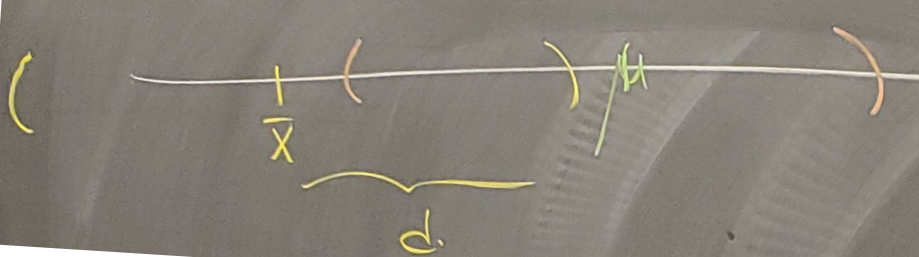
\includegraphics[width=5in]{10_3.png}\end{center}

\section{More about errors and sample size}

\nl \textbf{\color{eblue}Motivational example: } $X$ equals the breaking strength of a steel bar. If the bar is manufactured by Process I, it is known $X \sim N(50,\;36).$

\nl We now have Process II and it is hoped that the steel is 10\% stronger. i.e. $X \sim N(55,\;36)$.

\nl Our test? $$H_0 : \mu_I = 50 \hspace{1in} H_a : \mu_{II} = 55$$
{\red{Okay... we can't really test \say{this}}}

\nl But we can construct a hypothetical test where if $H_a$ is true, we can minimize (or control) both the Type I and Type II errors.

\nl For the sake of concrete-ness, set $n=16$. Then,
$$\sigma_{\Xbar}^2 = \frac{36}{16} \wideand \sigma_{\Xbar} = 1.5$$
\begin{center}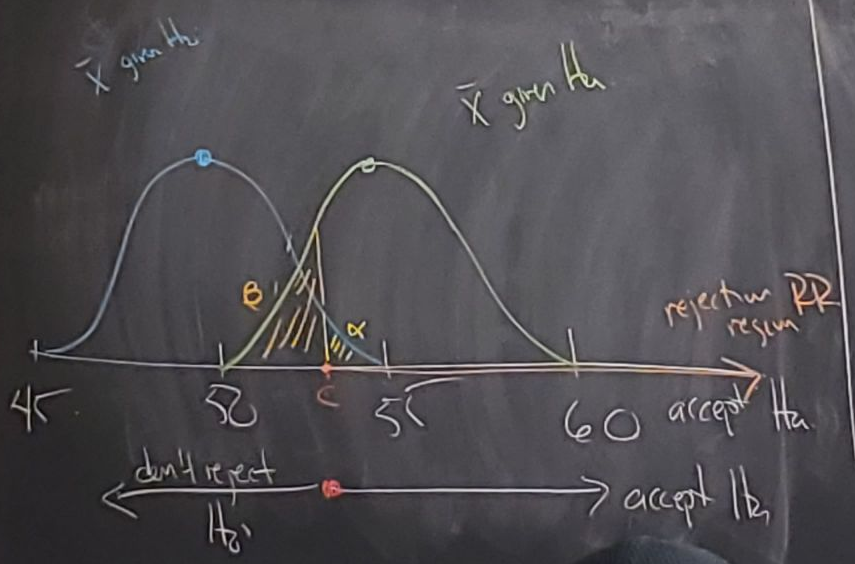
\includegraphics[width=6.5in]{2_25_1.png}\end{center}
$$\alpha = \P{\text{Type I}} \qquad H_0 : \mu = 50 \qquad H_a : \mu < 50$$
On the other hand, given $\alpha$, we can also see
$$\beta = \P{\text{Type II}} = \P{\text{accept } H_0 \text{ when } H_a \text{ is true}}$$


\nl Given $\alpha$, we can find $c$.
\begin{align*}
    \alpha &= \P{\Xbar > C \mid H_0}\\
    &= \P{\frac{\Xbar -{\color{blue}50}}{1.5} > \frac{C-{\color{blue}50}}{1.5}}
\end{align*}
and
\begin{align*}
    \beta &= \P{\Xbar < C \mid H_a}\\
    &= \P{\frac{\Xbar - {\color{ggreen}55}}{1.5} < \frac{C-{\color{ggreen}55}}{1.5}} 
\end{align*}
For fixed $n=16$, usually choose $\alpha$ small.
$$\alpha = \P{\Xbar -50 > 2\sigma_{\Xbar}} = 0.025$$%probably should be 1.960 instead of 2
Then $C = 50 + 2(1.5) = 53$ and
\begin{align*}
    \beta &= \P{\Xbar < 53 \mid H_a}\\
    &= \P{\frac{\Xbar - 55}{1.5} < 1.33}\\
    &= 0.0918
\end{align*}
Note almost four times as likely to make a Type II error than a Type I error. Of course, decreasing $\alpha$ with increase $\beta$.
$$\alpha = 0.01 \quad \implies \quad Z\text{-score} = 2.33 \qquad (Z_{0.98})$$
$$c = 50 + 2.33 (1.5) = 53.495$$
\begin{align*}
    \beta &= \P{\Xbar < 53.495 \mid H_a}\\
    &= \P{Z < -1.003}\\
    &= 0.1587
\end{align*}
Again, we note that the only way to decrease \textit{both} $\alpha$ and $\beta$ is to crank up the $n$.

\disc Choosing sample size $n$. We consider the 1-sided test
$$H_0 : \mu = \mu_0 \hspace{1in} H_a : \mu > \mu_0$$
Fix $\alpha$ at the start.
\begin{align*}
    \alpha &= \P{\Xbar > C \text{ when } \mu = \mu_0}\\
    &= \P{Z > \frac{C-\mu_0}{\sigma / \sqrt{n}}}\\
    &= \P{Z > Z_{\alpha}} \qquad Z_{\alpha} = \frac{C-\mu_0}{\sigma/\sqrt{n}}
\end{align*}
But, as with the power function, we need to choose specific $\mu_a$'s to work with (e.g. $\mu_a = 55$).
\begin{align*}
    \beta &= \P{\Xbar < C \text{ when } \mu = \mu_a}\\
    &= \P{Z < \frac{C-\mu_a}{\sigma / \sqrt{n}}}\\%
    &= \P{Z < -Z_{\beta}} \quad \text{when}\quad -Z_{\beta} = \frac{C-\mu_{\alpha}}{\sigma/\sqrt{n}}
\end{align*}
2 equations in the 2 unknows, $C,\;n$
$$C = \mu_0 + Z_{\alpha} \frac{\sigma}{\sqrt{n}} \wideand C = \mu_a - Z_{\beta} \frac{\sigma}{\sqrt{n}}$$
$$\mu + Z_{\alpha} \frac{\sigma}{\sqrt{n}} = \mu_a - Z_{\beta} \frac{\sigma}{\sqrt{n}} $$
Solve for $n$: 
$$(Z_{\alpha} + Z_{\beta})\frac{\sigma}{\sqrt{n}} = \mu_a - \mu_0$$
$$n = \frac{(Z_{\alpha} + Z_{\beta})^2 \sigma^2}{(\mu_a-\mu_0)^2}$$
Remark:
\begin{enumerate}[label=\textcircled{\raisebox{-1pt}{\arabic*}}]
    \item Of course all of this the fudge factor that we don't really know $\mu_a$.
    \item If we did $H_0 : \mu_0 = \mu_a$ and $H_a : \mu_0 > \mu_a$ we get the same formula for $n$. \say{sample size estimator for a one-sided $\alpha$-level test}
\end{enumerate}

\example* Back to the steel example

\nl If we decided at the start that we want $\alpha = \beta = 0.05$, what $n$ should we choose?

\nl For $\alpha = 0.05 \implies Z_{\alpha} = Z_{0.05} = 1.645$. Similarly for $\beta$, we need $Z_{\beta} = 1.645.$
Into our formula,
$$n = \pars{\frac{1.645+1.645}{\color{ggreen}55 \color{black} - \color{blue}50 \color{black}}}^2 \cdot 36 = \lceil 15.5867 \rceil = 16$$
Since we made $\alpha = \beta$ here, $C$ is the midpoint $C = \dfrac{55+50}{2} = 52.5$.
\begin{center}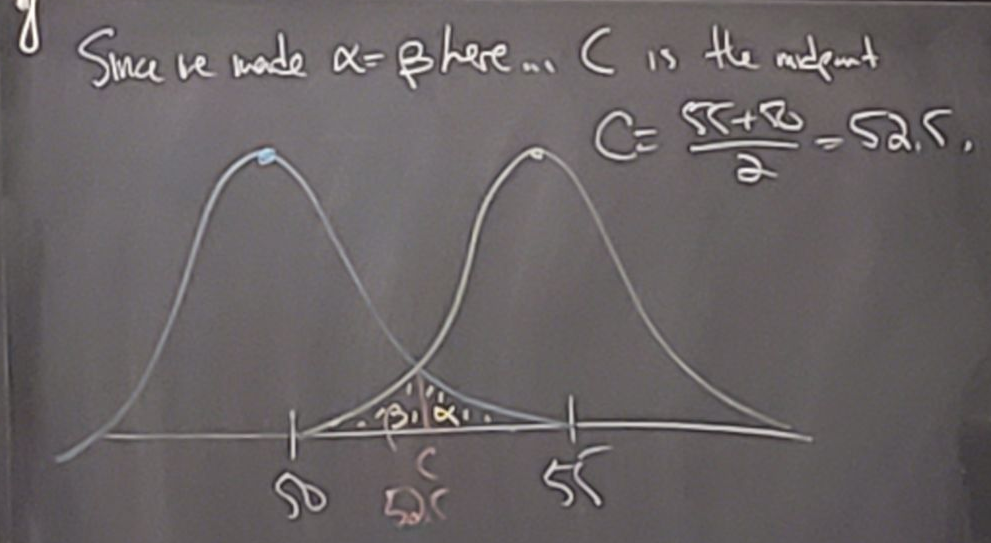
\includegraphics[width=4.5in]{2_25_2.png}\end{center}

\setSection{7}
\section{T tests} %10.8
Recall that for a small sample $n < 30$. We need to use the $t$-distribution.

\nl Chapter 8: t-stat confidence interval $\displaystyle \Xbar \pm t_{\alpha/2}(\text{df})\sqrt{\frac{s^2}{n}}$

\example 100 mL sample of water from swimming areas are tested for fecal colliform bacteria. It is considered to be safe if the level of bacteria is less than 400 in 3.3 oz.

\nl 20 Samples are taken: Found $\Xbar = 1231$ and $S = 1038$.

\nl Construct a test to determine if it's safe to swim. Our test:
\begin{align*}
    &H_0 : \mu_0 = 400\\
    &H_a : \mu_a > 400
\end{align*}
Test statistic $\displaystyle T = \frac{\Xbar - \mu_0}{S \big/ \sqrt{n}} = \frac{1231 - 1038}{1038\big/\sqrt{20}} = 0.350$ is the test statistic.

\nl The degrees of freedom is $n - 1 = 19$. Using table 5, $t_{0.005}(19)=2.861$ The $p$-value is: 
\begin{align*}
    p &= \Pr(T \geq 3.580 \mid \mu_0 = 400)\\
    &< \Pr(T \geq 2.861)\\
    &= 0.005
\end{align*}

\nl Reject $H_0$: There is poop in the water; stay out!

\remark* In general:
$$\displaystyle H_a := \begin{cases} \mu > \mu_0 \\ \setBlue \mu < \mu_0 \\ \setRed \mu \neq \mu_0 \end{cases} \implies \text{RR} := \underbrace{\begin{cases}t > t_{\alpha} \\ \setBlue t < -t_{\alpha}\\ \setRed \abs{t} > t_{\alpha/2} \end{cases}}_{\textstyle \text{the } t \text{-stat}}$$

\example Lifestyle comparison. Monitoring the active time (in minutes per day) between 2 populations: obese and lean.
\begin{center}
    \begin{tabular}{ |c|c|c|c| } 
        \hline
        \textbf{Group} & \textbf{Count} & \textbf{Standing/Walking} & $S$\\
        \hline
        Obese & $n=10$ & 373.269 & 67.498\\ 
        \hline
        Lean & $n=13$ &  525.751 & 107.121\\ 
        \hline
      \end{tabular}
    \end{center}


\nl Question: Are these two groups significant significant? This is a \say{are population means different} question.
\begin{align*}
    H_0 &: \mu_L = \mu_0 \quad \implies \quad  \mu_L - \mu_0 = 0\\
    H_a &: \mu_L \neq \mu_0 \quad \implies \quad \mu_L - \mu_0 \neq 0
\end{align*}
Questions about \say{\setRed different} results in a 2-sided test

\nl Confidence interval: $\displaystyle \Xbar_1 - \Xbar_2 \pm t_{\alpha/2}(\df)\pars{S_p\sqrt{\dfrac{1}{n_1} + \dfrac{1}{n_2}}}$
$$\color{orange} S_{\text{pool}} \setBlack = \sqrt{\dfrac{(n_1-1){S_1}^2 + (n_2-1){S_2}^2}{n_1 + n_2 - 2}} \quad \text{with } \df = n_1 + n_2 - 2$$
The difference in means $t$ test statistic is 
$$T = \dfrac{\Xbar_1 - \Xbar_2 - (\mu_1 - \mu_2)}{S_p \sqrt{\over*{n_1} + \over*{n_2}}}$$
Our $\Xbar_L - \Xbar_0 = 152.482$. $H_0 : \mu_L - \mu_0 = 0$ is the null hypothesis. $\df = 10+13-2=21.$
\begin{align*}
    S_p &= \sqrt{\dfrac{(13-1)107.121^2 + (10-1)67.498^2 }{13+10-2}}\\
    &= 92.247.\\
    \\
    T &= \frac{152.481}{92.247 \sqrt{\over*{10} + \over*{13}}}\\
    &= 3.93
    \\\\p &= \P{|T|>3.93} \\ &= 2 \cdot \P{T > 3.93}\\ &< 2 \cdot 0.0005 \tag{by table 5}\\
    & = 0.001
\end{align*}
So $p$ is super small ($p < \alpha$) which implies that we reject the null hypothesis. That is, $\mu_0 < \mu_L$ is true.

\nnl Our goal this week is to justify hypothesis testing. 

\nl Last day: Pearson Neyman Lamma

\nl $\thru{X} \sim$ via PDF $f(x \mid \theta)$ when $\theta_0$ and $\theta_a$ are two possible values of $\theta$. If there exists $a$ the constant $k$ and a subset $C$ of the sample space such that
\begin{enumerate}
    \item $P\{(\thru{x}) \in C \mid \theta_0\} = \alpha$
    \item $\dfrac{L(\theta_0)}{L(\theta_a)} \leq k$ for $\thru{x} \in C$.
    \item $\dfrac{L(\theta_0)}{L(\theta_a)} \geq k$ for $\thru{x} \in \overline{C}$
\end{enumerate}
Then $C$ is a best critical region of size $\alpha$ for testing $H_0 : \theta = \theta_0$ versus $H_a : \theta = \theta_a$.

\nl Before the proof\dots example.

\example Let $\thru{Y}$ from $\displaystyle f(y \mid \theta) = \frac{2}{\theta}y e^{-y^2/\theta}$ and $y > 0$. The Rayleight distribution.

\nl Want to test  $H_0 : \theta = \theta_0$ versus $H_a : \theta = \theta_a$.

\nl Note $\displaystyle L(\thru{Y} \mid \theta) = \frac{2}{\theta} y_i e^{-y_i^2/\theta} \cdots \frac{2}{\theta} y_n e^{-y_n^2/\theta}$.
$$\pars{\frac{2}{\theta}}^n \underbrace{\exp \brac{- \pars{\sum_1^n y_i^2} \bigg/ \theta }}_{g(S,\theta)} \underbrace{\prod_1^n y_i}_{h}$$
We will come back to this and connect to sufficiency next day.

The N-P ratio of likelihood function becomes
\begin{align*}
    \dfrac{L(\theta_0)}{L(\theta_a)} &= 
    \frac
    {\pars{\frac{2}{\theta_0}}^n \exp \brac{- \pars{\sum_1^n y_i^2} \bigg/ \theta_0 }\prod_1^n y_i}
    {\pars{\frac{2}{\theta_a}}^n \exp \brac{- \pars{\sum_1^n y_i^2} \bigg/ \theta_a }\prod_1^n y_i}\\
    &= \pars{\frac{\theta_a}{\theta_0}}^n \exp \brac{-\sum y_i^2 \cdot \pars{\over{\theta_0} - \over{\theta_a}}}
\end{align*}
We want $C$ to relate to our rejection region RR.

\nl So (2), implies \say{reject $H_0$ if}
$$\pars{\frac{\theta_a}{\theta_0}}^n \exp \brac{-\sum y_i^2 \cdot \pars{\over{\theta_0} - \over{\theta_a}}} \leq k$$
This looks scary, but $\theta_a$ and $\theta_0$ are fixed and $\theta_0 < \theta_a$ so $\pars{\over{\theta_0} - \over{\theta_a}} > 0$. In the end, making $\dfrac{L(\theta_0)}{L(\theta_a)}$ \say{small enough} for $k$ simlifies does to the condition that $\sum_{i}^n y_i^2$ is large enough. i.e. we need $\sum_1^n y_i^2 > k'$ for some $k'$ (dependent upon $k$). 

\nl New problem: To determine an appropriate $k'$, we need to know how $S = \sum_1^n y_i^2$ is distributed. 

\nl Using CDF method ($\S$ 6.3) we can show that the distribution of $y^2$ is exponention with mean $\theta$. Then, via products of moment generating functions. $$S = \sum_1^n y_i^2 \sim \operatorname{Gamma}\pars{n, \over{\theta}}$$
Stop! What just happened. 

\nl The N-P lemma tells us that the most powerful test of $H_0$ vs $H_a$ is to use the statistic $S = \sum y_i^2$. Then, given any $\alpha$ level significance (5\%, 1\%, whatever), we use the test on $S$ to be if $S$ is larger than $100(1-\alpha)$ percentile of the $\operatorname{Gamma}\pars{n, \over{\theta}}$ distribution\dots we reject $H_0$. 

\nl Picture with some $\gamma_*$ such that $\int_{\gamma_*}^{\infty} = \alpha$.

\nl $S > \gamma_*$, we reject the null hypothesis. Moreover, by the NP lemme, we don't have to compare the powe rof other possible tests because the lemma says any data
$$(\thru{Y}) \in C \leftrightsquigarrow S \geq \gamma_*$$
$$C := \left\{ (\thru{Y}) \mid \sum y_i^2 \geq \gamma_* \right\}$$
which is itself a consequence of our significance level $\alpha$ results in the most powerful test. 
$$P(C \mid \theta_a) \geq P(D \mid \theta_a)$$
where $D$ is another critical region $(P(D \mid \theta_a) = \alpha )$.

\defn The test using the best critical region is called the most powerful test. 

\nl Recap: We wanted to construct a hypothesis test at $\alpha$ significance level. All in one fell swoop, the N-P lemme says
\begin{enumerate}
    \item Here is the stat to use ($S = \sum y_i^2$ in last example) 
    \item Here is your rejection region ($S \geq \gamma_a$ in last example)
    \item in fact, this is the most powerful test possible.
\end{enumerate}
(This is kinda awesome)

Theorem: NP lemma;
\begin{proof} (Continuous)\\
    Let $B \subseteq \R^n$ and define $\displaystyle \underbrace{\int_B L(\theta) = \int \cdots \int}_{n \text{times}} L(\thru{x} \mid \theta) \, dx_1\, dx_2, \dots, dx_n  $.\\
    Assume there exists a critical region $C$ satisfying bullets 1 2 and 3.

    \nl $\alpha$ fixed, $\alpha = \int_C L(\theta_0)$ (same as $P(C \mid \theta_0)$)

    \nl Need to prove \say{best}, i.e. $P(C \mid \theta_a) \geq P(D \mid \theta_a)$

    \nl Assume $D$ is another critical region,
    $$\alpha = \int_D L(\theta)_0 = P(D\mid \theta_0)$$
    So $\displaystyle 0 = \int_C L(\theta_0) - \int_D L(\theta_0) $
    \begin{align*}0 &= \int_{C \cap D^C} L(\theta_0) + \int_{C \cap D} L(\theta_0) - \brac{ \int_{C \cap D} L(\theta_0) + \int_{C^C \cap D} L(\theta_0) }\\
        &= \int_{C \cap D^C} L(\theta_0) - \int_{C^C \cap D} L(\theta_0)\\
    &\text{By (2), there exists $k$ such that $\dfrac{L(\theta_0)}{L(\theta_a)} \leq k$ i.e. $L(\theta_0) \leq kL(\theta_a)$ at every point in $C$.}\\
    & \leq k \int_{C \cap D^C} L(\theta_a) - \int_{C^C \cap D} L(\theta_0)\\
    &\text{By (3) there exists $k$ such that $\dfrac{L(\theta_0)}{L(\theta_a)} \geq k$ i.e.  $L(\theta_0) \geq kL(\theta_a)$}\\
    & \leq k \brac{\int_{C \cap D^C} L(\theta_a) - \int_{C^C \cap D} L(\theta_a)}\\
    &= k \brac{\int_{C \cap D^C} L(\theta_a) + \int_{C \cap D} L(\theta_a) - \brac{ \int_{C \cap D} L(\theta_a) + \int_{C^C \cap D} L(\theta_a) }}\\
    &= k \brac{\int_C L(\theta_a) - \int_D L(\theta_a)}\\
    & \implies \int_C L(\theta_a) - \int_D L(\theta_a) \geq 0\\
    & \implies \int_C L(\theta_a) \geq \int_D L(\theta_a)\\
    & \implies P(C \mid \theta_a) \geq P(D \mid \theta_a)
    \end{align*}
    Here, $C$ is a best critical region of size $\alpha$ by defininition.
\end{proof}
\example Back to our old sample size example. 
$$\thru{X} \sim \operatorname{N}(\mu,\,36)$$
We played with $H_0 : \mu = 50$ and $H_a : \mu = 55$. 

\nl Consider the ratio of the likelihood functions.

\begin{align*}
    \frac{L(50)}{L(55)}
    &= \dfrac{(72 \pi)^{-n/2} \exp \brac{-\pars{\over{72}} \sum_1^n (X_i - 50)^2} }{{(72 \pi)^{-n/2} \exp \brac{-\pars{\over{72}} \sum_1^n (X_i - 55)^2} }}\\
    &= \exp \brac{ - \over{72} \sum_1^n \brac{(X_i-50)^2-(X_i-55)^2}}\\
    &= \exp \brac{-\over{72} \sum_1^n (10X_i -525) }\\
    &= \exp \brac{-\frac{5}{36} \sum_1^n X_i + \frac{175n}{24}} \leq k \text{ to satisfy (2)}\\
    & \implies -\frac{5}{36} \sum_1^n X_i + \frac{175n}{24} \leq \ln k\\
    & \implies \sum_1^n X_i \geq \frac{105n}
    {2} - \frac{36}{5} \ln k
    \\ & \implies \Xbar = \over{n}\sum_1^n X_i \geq \frac{105}{2} - \frac{36\ln k}{5n}
\end{align*}
We have our stat $\Xbar \geq k'$ thus will define our rejectoin rejection.

    %\text{    By (2), there exists $k$ such that $\dfrac{L(\theta_0)}{L(\theta_a)} \leq k$ i.e. $L(\theta_0) \leq kL(\theta_a)$ at every point in $C$.

    %By (3) there exists $k$ such that $\dfrac{L(\theta_0)}{L(\theta_a)} \geq k$ i.e.  $L(\theta_0) \geq kL(\theta_a)$}




% ^  stuff to finish









\chapter{Linear Models and Estimation by Least Squares}
\section{Introduction} We are going to do best-fit lines in 2 separate ways.

\nl Consider some sample (data) $S = \{(x_i,\, y_i)\}$. In the background, there can be an underlying joint PDF $f(x,y)$
\begin{center}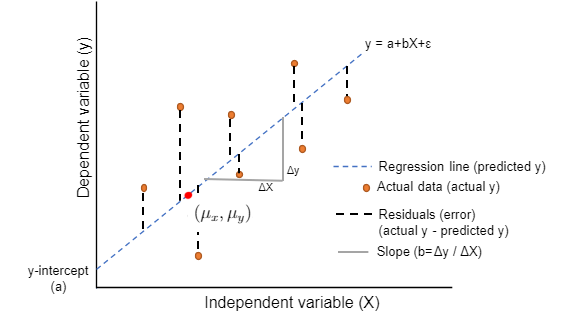
\includegraphics[width=4in]{ch11_regression.png}\end{center}
\section{Linear Statistical Models}

\noindent Assumptions
\begin{enumerate}[label=\textcircled{\raisebox{-1pt}{\arabic*}}]
    \item $Y$ is dependent upon $X$. (i.e. not an independent random variable.)
    \item In general, $y = mx + b$, the general relationship between $X$ and $Y$.
\end{enumerate} 

\newpage
\section{The Method of Least Squares}
\nl\textbf{A.) The probabalistic construction:}

\nl Given all possible lines $y=mx+b$ that \textit{could} describe the data, the \say{most likely} one will be a line that intersects the point $(\mu_x, \mu_y)$.

\nl That is $y - \mu_y = m(x-\mu_x)$. Because we are interpreting $y$ and a function of $x$, the \say{best line} should be one that minimizes the vertical distance (error (residuals)) in the $y$-direction.

\nl For a point $(x_k,\, y_k)$ in $S$, the vertical distaince is 
$$\text{dist} = \abs{y_k - \big(m(x_k - \mu_x) + \mu_y \big)}.$$
Minimizing absolute values is a pain, but calculus I suggests we square this,
$$\operatorname{dist}^2 = \Big((y_k-\mu_y) - m(x_k-\mu_x)\Big)^2.$$
As $x,y$ are distributed via some PDF, the best way to compute our minimization problem is to minimize expectation with respect to slope $m$:
$$K(m) := \E{\operatorname{dist}^2(m)} = \underbrace{\E{\Big((y_k-\mu_y) - m(x_k-\mu_x)\Big)^2}}_{\setRed **}.$$
\setRed ** \setBlack The $m$ that minimizes is called the solution to our \underline{least-squares problem}.
\begin{align*}
    K(m) &= \E{(y_k-\mu_y)^2  -2m(x_k-\mu_x)(y_k - \mu_y) + m^2(x_k-\mu_x)^2 }\\
    &= \E{(y_k-\mu_y)^2} -2m \E{(x_k-\mu_x)(y_k - \mu_y) } + m^2\E{(x_k-\mu_x)^2}\\
    &= S^2_y - 2m \Cov(X,Y) + m^2S^2_x
\end{align*}
Minimizing (with respect to $m$) $\dfrac{\partial}{\partial m}$,
$$K'(m) = -2 \Cov(X,Y) - 2mS^2_x.$$
With $K'(m) = 0$ then $m = \dfrac{\Cov(X,Y)}{S^2_x}$. 

\nl Note that by the second derivitive test, $K''(m) = 2S_x^2 > 0$. In AP Stats (MTH 111), the slope is moved to a \say{prettier} form:

\begin{align*}
    m &= \frac{\Cov(X,Y)}{S_x^2} \\
    &= \frac{\Cov(X,Y)}{S_x S_y} \cdot \frac{S_y}{S_x}\\
    &= \rho \cdot \frac{S_y}{S_x} \hspace{1in} \rho := \frac{\Cov(X,Y)}{S_xS_y}
\end{align*}

\nl \bu{FACT \#1}: The sign of the slope depends entirely upon $\rho$, where the sign is dependent upon $\Cov(X,Y)$

\nnl \bu{FACT \#2}: $-1 \leq \rho \leq 1$.

\nl (For my MTH 325 class, we proved this fact in full generality).

\nnl \bu{FACT \#3}: The closer $\abs{\rho}$ is to 1, the better the line $\widehat{y} = mx+b$ \say{fits} the data.
\begin{center}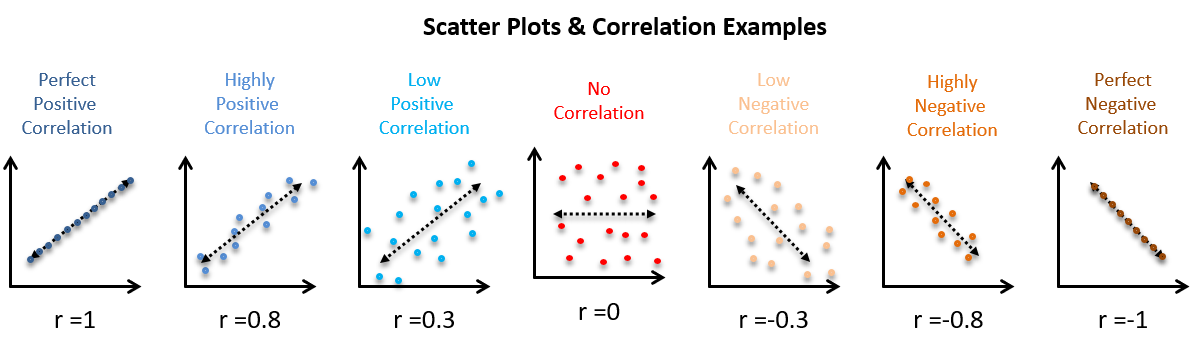
\includegraphics[width=6in]{ch11_scatter.png}\end{center}

\nl The AP Stats definition fo the best fit line is $\widehat{y} = \widehat{b}_0 + \widehat{b}_1x$ where $\widehat{b}_1 = \rho \dfrac{S_y}{S_x}$ and $\widehat{b}_0 = \bar{y} - \widehat{b}_1 \bar{x}$.

\nnl\textbf{B.) The linear algebra construction:}

\nl We still have $S = \{(x_k,\, y_k)\}$. We want $y = mx+b$. Using $S$ always yields an overdetermined (i.e. inconsistent) system
\begin{align*}
    y_1 &= mx_1 + b\\
    y_2 &= mx_2 + b\\
    & \;\;\vdots\\
    y_n &= mx_n + b.
\end{align*}
This is $n$ equations with 2 variables, but we can rewrite as vector equations. $$\vec{y} = m\vec{x} + b \vec{1} \quad \text{where } \vec{y} = \thru{y}, \vec{x} = \thru{x}, \text{ and } \vec{1} = \underbrace{(1,1,\dots,1)}_{n \text{ components}}.$$

\nl Trying to write $\vec{y}$ as a linear combination of $\vec{x}$ and $\vec{1}$. Consider the plane $P = \operatorname{span}\{\vec{x},\vec{1}\}$. Inconsistent implies that $\vec{y} \not \in P$.

\nl But the vector in $P$ that is closest to $\vec{y}$ is $\operatorname{proj}_P\vec{y}$. (Closest under Euclidean distance), recall $\inner{u,v} = u \cdot v$ in $\R^n$.
$$\operatorname{dist}^2 = \sum (y_i - v_i)^2, \quad \vec{v} \in P = \underbrace{\vec{y} \cdot \vec{v} = \inner{y,v}}_{\substack{\text{\say{least squares}}}}$$
\begin{center}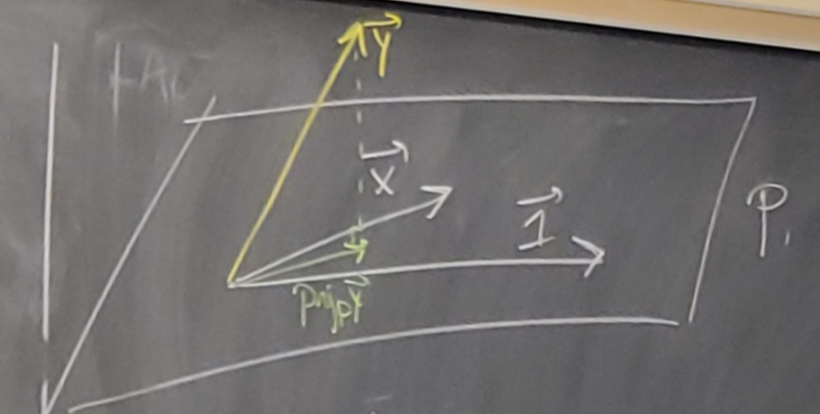
\includegraphics[width=4in]{ch11_proj.png}\end{center}

\noindent Easiest way to project onto $P$ is to have an orthogonal basis for $P$. We need an orthogonal basis for $P$: 
\begin{center}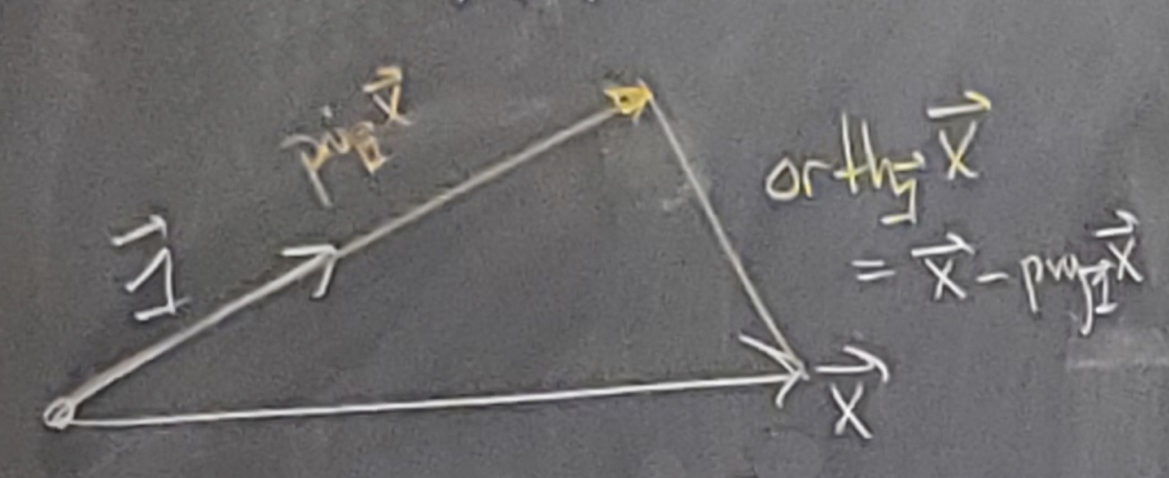
\includegraphics[width=4in]{ch11_basis.png}\end{center}

\nl $P = \operatorname{span}\left\{1, \, \operatorname{orth}_{1}x \right\} = \operatorname{span}\left\{1,\, v\right\}$ where
\begin{align*}
    v &= x - \proj{1}{x}\\
    &= x - \frac{\inner{x,1}}{\inner{1,1}}{1}\\
    &= x - \frac{\inner{x,1}}{n}{1}
\end{align*}
Then 
\begin{align*}
    \proj{P}{y} &= \frac{\inner{y,1}}{\inner{1,1}}1 + \frac{\inner{y,v}}{\inner{v,v}} v\\
    &= \frac{\inner{y,1}}{n}{1} + \frac{\inner{y,v}}{\inner{v,v}}x -\frac{\inner{y,v}}{\inner{v,v}} \cdot \frac{\inner{x,1}}{n}{1}\\
    &= \underbrace{\frac{\inner{y,v}}{\inner{v,v}}}_{\setGreen\substack{\textstyle m\\  \textstyle\text{(slope)}}}x + \underbrace{\pars{\frac{\inner{y,1}}{n} - \frac{\inner{y,v}}{\inner{v,v}}\cdot\frac{\inner{x,1}}{n}}}_{ \setGreen \substack{\textstyle b\\\textstyle\text{(}y \text{-intercept)}}}1
\end{align*}

\begin{align*}
    \inner{v,v} &= \inner{x - \frac{\inner{x,1}}{n}1,\; x - \frac{\inner{x,1}}{n}1}\\
    &= \inner{x,x} -2 \inner{x,\; \frac{\inner{x,1}}{n}1} + \inner{\frac{\inner{x,1}}{n}1,\; \frac{\inner{x,1}}{n}1}\\
    &= \inner{x,x} - 2 \frac{\inner{x,1}}{n}\inner{x,1} + \frac{\inner{x,1}^2}{n^2}\inner{1,1}\\
    &= \inner{x,x} - 2 \frac{\inner{x,1}^2}{n} + \frac{\inner{x,1}^2}{n}\\
    &= \frac{n \inner{x,x} - \inner{x,1}^2}{n}
    %
    %&= \inner{x,x} - 2 \frac{\inner{x,1}^2}{n} + \inner{\frac{\inner{x,1}^2}{n^2}1 ,\; 1}\\
    %&= x \cdot x - 2 \frac{\inner{x,1}^2}{n} + \frac{\inner{x,1}^2}{n}\\
    %&= \frac{n\inner{x,n} - \inner{x,1}^2}{n}
\end{align*}

\begin{align*}
    \inner{v,y} &= \inner{x,y} - \frac{\inner{x,1}\inner{y,1}}{n}\\
    &= n\inner{x,y} - \inner{x,1}\inner{y,1}
\end{align*}
Then
\begin{align*}
    m &= \frac{\inner{v,y}}{\inner{v,v}}\\
    &= \setBlue\frac{n\inner{x,y} - \inner{x,1}\inner{y,1}}{n\inner{x,x} - \inner{x,1}^2}
\end{align*}

% ^^^^ monday to finish

\noindent Then % b = (y dot 1 / n)    -    m (x dot 1 / n)
\begin{align*}
    b &= \frac{\inner{y,1}}{n} - m \frac{\inner{x,1}}{n}\\
    &= \bar{y} - m \bar{x}
\end{align*}
Which is what we got form the probabalistic approach.

\nnl Claim: The two-sets of formulas are identical

\begin{align*}
    m &= \frac{\Cov(X,Y)}{S_x^2} = \rho \frac{S_y}{S_x}\\
    &= \frac{\sum(x_i-\bar{x})(y_i-\bar{y})}{\sum (x_i - \bar{x})^2}
\end{align*}
Useful formula:
\begin{align*}
    \sum (x_i - \bar{x})(y_i - \bar{y}) &= \sum (x_i y_i - x_i \bar{y} - y_i \bar{x} + \bar{x}\bar{y})\\
    &= \sum x_i y_i - \bar{y} \sum x_i - \bar{x} y_i + \bar{x}\bar{y} \sum 1\\
    &= \sum x_i y_i - \bar{y} n \cdot \over{n} \sum x_i - \bar{x} n \cdot \over{n} \sum y_i + n \bar{x} \bar{y}\\
    &= \sum x_iy_i - n \bar{x} \bar{y} -  n\bar{x} \bar{y} +  n\bar{x} \bar{y}\\
    &= \sum x_i y_i - n\bar{x} \bar{y}
\end{align*}

\begin{align*}
    m &= \frac{\Cov(X,Y)}{S_x^2} = \rho \frac{S_y}{S_x}\\
    &= \frac{\sum(x_i-\bar{x})(y_i-\bar{y})}{\sum (x_i - \bar{x})^2}\\
    &= \frac{\sum x_iy_i - n  \bar{x} \bar{y}}{\sum x_i^2 - n \bar{x}^2}\\
    &= \frac{\inner{x,y} - n \pfrac*{\inner{x,1}}{n} \pfrac*{\inner{y,1}}{n} }{\inner{x,x} - n \pfrac*{\inner{x,1}}{n}^2}\\
    &= \setBlue \frac{n\inner{x,y} - \inner{x,1}\inner{y,1}}{n \inner{x,x} - \inner{x,1}^2}\\
    &= \frac{n\sum x_i y_i - \pars{\sum x_i}\pars{\sum y_i}}{n \sum x_i^2 - \pars{\sum x_i}^2}\\
    &= m
\end{align*}


\setSection{3}
\section{Properties of the Least-Squares Estimators: Simple Linear Regression}

\nl The Coefficents of the Best-Fit Line are Estimators. We have shown the best-fit line to be $\displaystyle \widehat{y} = \widehat{\beta_0} + \widehat{\beta_1}x$.

\nl Where $\displaystyle \widehat{\beta_1} = \dfrac{S_{xy}}{S_{xx}}$ with $S_{xy} = \sum (x_i - \bar{x})(y_i - \bar{y})$ and $S_{xx} = \sum (x_i - \bar{x})^2$. (i.e. $\Cov(X,Y)$ and $\Vb{X}$ via use of $\bar{x}$, $\bar{y}$ for $\mu_x$, $\mu_y$ ).

\nl $\displaystyle \widehat{\beta_0} = \bar{y} - \widehat{\beta_1}x$

\nl We recognize $\widehat{\beta_0}$ and $\widehat{\beta_1}$ as stats dependent upon $\bar{x}, S_x^2,$ and $\bar{y}$.


\nnl But what exactly are they estimating? In theory, $X \times Y$ distributed via pdf $f(x,y)$ and there is some \say{best} linear relationship over the same probabilty space. 
$$y = \beta_0 + \beta_1 x.$$

\nl In other words, when we are \say{at} $x_i$,
$$\Eb{Y} = \beta_0 + \beta_1 x_i.$$

\nl A modern approach to the distribution of $Y$ at $x$ is to add an error parameter $\red{\varepsilon}$. That is,
$$\setGreen y = \setBlack \underbrace{\setGreen \beta_0 + \beta_1 x}_{\substack{ \text{deterministic}\\\text{component}\\\text{of } Y}}
+ \underbrace{\red{\varepsilon}}_{\substack{\text{\say{random}}\\ \text{component}}}$$

\nl Still want $\Eb{Y} = \beta_0 + \beta_1 x$. By linearity,

\begin{align*}
    \Eb{Y} &= \Eb{\beta_0 + \beta_1x + \varepsilon}\\
    &= \Eb{\beta_0 + \beta_1x} + \Eb{\varepsilon}\\
    &\implies \Eb{\varepsilon} = 0 \quad \text{error averages to zero}
\end{align*}

\nl We make the additional assumption that the variance of $\varepsilon$ is independent of $x$. That is $\Vb{Y} = \Vb{\varepsilon} = \sigma^2$. The \say{value} of $y$ \textit{depends} on $x$, but the spread of the $y$-values does not.

\nnl\textbf{Proposition:} $\widehat{\beta_0}, \widehat{\beta_1}$ are unbiased estimators of $\beta_0, \beta_1$ where $Y = \beta_0 + \beta_1x + \varepsilon$.

\nl \textbf{Reason:} 
\begin{align*}
    \E*{\widehat{\beta_1}} &= \Eb{\frac{S_{xy}}{S_{xx}}}\\
    &= \Eb{\frac{\sum (x_i - \bar{x})(y_i - \bar{y})}{S_{xx}}}\\
    &= \Eb{\frac{\sum (x_i - \bar{x})y_i - \sum (x_i - \bar{x})\bar{y}}{S_{xx}}}\\
    &= \Eb{\frac{\sum(x_i - \bar{x})y_i - \overbrace{\bar{y} \sum(x_i - \bar{x})}^{0 \text{ by def'n of } \bar{x}}}{S_{xx}}}\\
    &= \Eb{\frac{\sum (x_i - \bar{x})y_i}{S_{xx}}}\\
    &= \frac{\sum (x_i - \bar{x}) \E*{y_i}}{S_{xx}}\\
    &= \frac{\sum (x_i - \bar{x}) \setGreen{(\beta_0 + \beta_1 x_i)}}{S_{xx}}\\
    &= \frac{\overbrace{\beta_0 \sum (x_i - \bar{x})}^{0} + \beta_1 \sum (x_i - \bar{x})x_i}{S_{xx}}\\
    &= \frac{\beta_1 \sum (x_i^2 - x_i \bar{x})}{S_{xx}}\\
    &= \frac{\beta_1 \pars{\sum x_i^2 - \bar{x} \sum x_i}}{S_{xx}}\\
    &= \frac{\beta_1 \pars{\sum x_i^2 - n\bar{x}^2}}{S_{xx}}\\
    &= \beta_1 \frac{S_{xx}}{S_{xx}}\\
    &= \beta_1
\end{align*}
Therefore our estimator is unbiased.

\nl The point of all that: $\E*{\widehat{\beta_1}} = \widehat{\beta_1}$.

\nl For $\E*{\widehat{\beta_0}} = \Eb{\bar{y} -\widehat{\beta_1} \bar{x}} = \Eb{\bar{y}} - \bar{x} \E*{\widehat{\beta_1}}$.

\nl But $\displaystyle \bar{y} = \over{n} \sum y_i = \over{n} \sum (\beta_0 + \beta_1 x + \varepsilon) = \beta_0 + \beta_1 \bar{x} + \varepsilon$.

\nl and $\Eb{\bar{y}} = \beta_0 + \beta_1 \bar{x}$. and $\Eb{\widehat{\beta_0}} = \beta_0 + \beta_1 \bar{x} - \beta_1 \bar{x} = \beta_0$.


\nnl \textbf{Corollary:} $\displaystyle \Var*{\widehat{\beta_1}} = \dfrac{\sigma^2}{S_{XX}}, \Var*{\widehat{\beta_0}} = \frac{\sigma^2 \sum x_i^2}{nS_{XX}} $.

\nl \textbf{Reason} 
\begin{align*}
    \Var*{\widehat{\beta_1}} &= \Var{\dfrac{\sum(x_i-\bar{x})(y_i - \bar{y})}{\sum(x_i-\bar{x})^2}}\\
    &= \Var{\dfrac{\sum(x_i-\bar x)^2y_i}{S_{XX}}}\\
    &= \over{{S_{XX}}^2} \Var{\sum (x_i-\bar x)y_i}\\
    &= \frac{\sum (x_i - \bar x)^2 \Var{Y_i}}{{S_{XX}}^2}
    \\ \text{assumption: } \Var{Y} = \Var{\varepsilon} = \sigma^2\\
    &= \frac{\sum (x_i - \bar x)^2 \sigma^2}{{S_{XX}}^2}\\
    &= \frac{\sigma^2 \sum(x_i - \bar x)^2}{{S_{XX}}^2}\\
    &= \frac{\sigma^2 S_{XX}}{{S_{XX}}^2} \\
    &= \frac{\sigma^2}{S_{XX}}.
\end{align*}

\begin{align*}
    \Var*{\widehat{\beta_0}} &= \Var{\bar y - \widehat{\beta_1} \bar x}\\
    \text{Note in our } \varepsilon & \text{ set up, } \bar y \text{ and } \widehat{\beta_1} \text{ both functions of } Y_i\text{'s\dots may be independent.}
    \\ &= \Var {\bar y} - \Var*{\widehat{\beta_1} \bar x} - 2 \Cov (\bar y, \widehat{\beta_1}\bar x)\\
    &= \Var{\bar y} + \bar x^2 \Var*{\widehat{\beta_1}} - 2\bar x^2 \Cov (\bar y, \widehat{\beta_1})
\end{align*}
And i.) $\displaystyle \Var{\bar y} = \Var{\bar{\varepsilon}} = \over{n} \Var{\varepsilon} = \over{x} \sigma^2$.
And ii.)
\begin{align*}
    \Cov (\bar y, \widehat{\beta_1}) &= \Cov \pars{\over{n}\sum y_i,\; \sum \frac{(x_i - \bar x)y_i}{S_{XX}}}\\
    &= \sum \frac{(x_i - \bar x) \Var{Y_i}}{nS_{xx}} + \sum \sum_{i \neq j} \frac{(x_j 0 \bar x)}{n S_{XX}} \underbrace{\Cov (Y_i, Y_j)}_{\text{independent } = 0}\\
    &= \frac{\sigma^2}{n S_{XX}} \sum (x_i - \bar x)\\
    &= 0.
\end{align*}
Then 
\begin{align*}
    \Var*{\widehat{\beta_0}} &= \Var{\bar y} + \bar x^2  \Var*{\widehat{\beta_1}} - 2 \bar x^2 \Cov (\bar y, \widehat{\beta_1})\\
    &= \frac{\sigma^2}{n} + \bar x^2 \cdot \frac{\sigma^2}{S_{XX}}\\
    &= \sigma^2 \pfrac{S_{XX}+n \bar x^2}{nS_{XX}}
\end{align*}

\begin{align*}
    S_{XX} &= \sum (x_i - \bar x)^2\\
    &= \sum(\bar x^2 - 2 \bar x) + \sum {x_i}^2\\
    &= n \bar x^2 - 2\bar x \sum x_i\\
    &= n \bar x^2 - 2 \bar x n \pfrac{\sum x_i}{n} + \sum {x_i}^2\\
    &= \sum {x_i}^2 - n \bar x^2 \qquad \text{i.e. } n \bar x^2 = \sum {x_i}^2 - S_{XX}
\end{align*}

\begin{align*}
    \Var*{\widehat{\beta_0}} &= \sigma^2 \pfrac{S_{XX} + \sum {x_i}^2 - S_{XX}}{n S_{XX}}\\
    &= \frac{\sigma^2 \sum {x_i}^2}{n S_{XX}}
\end{align*}

\nl Corollary: $\Cov (\widehat{\beta_0}, \widehat{\beta_1}) = - \frac{\bar x \sigma^2}{S_{XX}}$. Proof in textbook. Note: $\widehat{\beta_0}, \widehat{\beta_1}$ guaranteed to be dependent when $\bar x=0$.

\nnl \textbf{Topic: } estimating $\sigma^2$.

\nl We have working with the assumption that $\Var y = \Var{\varepsilon} = \sigma^2$, but this is usually unknown.

\nl In the past, we used $\displaystyle \Var Y = \over{n-1} \sum (y_i - \bar y)^2$.

\nl In our new setup, our point estimator for $y_i$ is no longer $\bar y$. Our estimator of $Y_i$ is the best-fit line: $\E{Y_i} = \widehat{\beta_0} + \widehat{\beta_1}x.$

\nl We define $S^2$ via sum square error
$$\operatorname{SSE} = \sum_{i=1}^n (y_i, \widehat{y_i})^2.$$
The term inside the summation is the residual; it is the error between the prediction and observed.
%residual pic

\nl We need to define an unbiased estimator for $\sigma^2$. Let 
\begin{align*}
    \that &:= K \cdot \operatorname{SSE} \\
    &= K \sum (y_i - (\widehat{\beta_0} + \widehat{\beta_1}x_i))^2
\end{align*}
By computing $\E*{\that}$, we choose $K$ so that $\E*{\that} = \sigma^2.$

\nl As we did in chapter 9, we can show that $\E*{\operatorname{SSE}} = (n-2) \sigma^2$. So, 
$$\boxed{S^2 = \over{n-2} \operatorname{SSE} = \over{n-2} \sum_{i=1}^n (y_i - \widehat{y_i})^2}$$

\nnl \textbf{Proposition: } $\E*{S^2} = \sigma^2$, (unbiased estimator).\\(aside: It would be nice to have a computation corollary like we did, i.e. $\Var{x} = \E{x^2} - \E x^2$)

\nl \textbf{Corollary: } The computation corollary
$$\operatorname{SSE} = S_{YY} - \widehat{\beta_1} S_{XY}$$
$$\text{where} \quad S_{YY} = \sum_{i=1}^n (y_i - \bar y)^2.$$

\example (11.16)\\
Potnecy of antibiotic ($y$): $(38,43,29), (32,26,33), (19,27,27), (14,19,21)$
\\After storage at $x^{\circ}$F: $30, 50, 70, 90$

$$\bar y = 27, \qquad \bar x = 60$$
$$S_{xy} = \sum (x_i-\bar x)(y_i i \bar y) = -1900$$
$$S_{xx} = \sum (x_i - \bar x)^2 = 6000$$
$$S_{yy} = \sum (y_i - \bar y)^2 = 792$$
Then $\widehat{\beta_1}= \dfrac{S_{xy}}{S_{xx}} = -\dfrac{19}{60}$ and $$\widehat{\beta_0} = \bar y - \widehat{\beta_1} \Xbar x = 27 - \pfrac*{-19}{60}60 = 46.$$
So the best fit line is $\widehat y = 46 - \frac{19}{60}x$. For 
\begin{align*}
    S^2 &= \over{n-2}\operatorname{SSE}\\
    &= \over{n-2}\pars{S_{yy}-\widehat{\beta_1}S_{xy}}\\
    &= \over{12-2}\pars{792 - \pfrac{-19}{60}(-1900)} = \frac{571}{30}
    \\ &\approx 19.0\overline{3}
\end{align*}

\disc Do we know how $S^2$ is distributed? This depends on our assumption on how $\varepsilon$ is distributed. 
$$y = \beta_0 + \beta_1 x + \varepsilon.$$
We have $\E*{\varepsilon} = 0$ and $\Var*{\varepsilon} = \sigma^2$, and thus are independent of $X$. 

\nl Note that the distribution of the point estimators $\widehat{\beta_0}$ and $\widehat{\beta_1}$ are $\sigma^2$ dependent (which we will estimate with $S^2$).

\nl However, the common assumption is that \say{everything} is normal! We assume $\varepsilon \sim \operatorname{N}(0, \sigma^2)$.

\nl We can now prove a Fisher's Theorem like result for the new $S^2$. 

\nl Namely\dots Theorem: $\displaystyle \frac{(n-2)S^2}{\sigma^2} = \frac{\operatorname{SSE}}{\sigma^2} \sim \chi^2(n-2)$, moreover $S^2$ is independent of $\widehat{\beta_0}$ and $\widehat{\beta_1}$. Proof: Omitted for mental health reasons. 
\section{Inferences concerning the point estimators}

\noindent Under the assumption $\varepsilon \sim \operatorname{N}(0,\sigma^2)$, we have that $\widehat{\beta_0}$ and $\widehat{\beta_1}$ are normal $\operatorname{N}(\beta_i, \Var*{\beta_i})$. Thus we can do confidence intervals for the true $\widehat{\beta_0}$ and $\widehat{\beta_1}$.
$$y = \beta_0 + \beta_1 x + \varepsilon$$
Use the same $\mathcal Z / \mathcal T$ rules as before, ($n \leq 30$ use $\mathcal T$ and $n > 30$ use $\mathcal Z$).

\nl As always, the standardization is 
$$\frac{\that - \theta}{\sqrt{\sigma_{\that}}} = \frac{\that - \theta}{\sqrt{\Var*{\that}}}$$

\example Given $Z_{\alpha/2}$ ($n > 30$), $\widehat{\beta_1} \pm Z_{\alpha/2}\sqrt{\Var*{\widehat{\beta_1}}}$ is an $\alpha$-level 2-sided C.I. for the true $\beta_i$.

\example Find a 90\% C.I. for the slope $\widehat{\beta_1}$ of the potency example. We have $\widehat{\beta_1} = \dfrac{-19}{60} \approx -0.3166\overline{7}$. 
\begin{align*}
    \Var*{\widehat{\beta_1}} &= \frac{\sigma^2}{S_{xx}}\\
    &\approx \frac{S^2}{S_{xx}}\\
    &= \frac{19.03}{6000}\\
    &= 0.00317\\
    \implies & S_{\widehat{\beta_1}} = \sqrt{\Var*{\widehat{\beta_1}}} = 0.0563
\end{align*}
Using $S^2$ implies we use $S^2$ degrees of freedom, $n=12$ implies $10$ degrees of freedom. Thus $S^2 \sim \chi^2(10)$. We need $t_{0.05}(10) = 1.812$ by table and 
\begin{align*}
    & \widehat{\beta_1} \pm t_{0.05}(10)S_{\widehat{\beta_1}}\\
    &- 0.31667 \pm (1.812)(0.0563)\\
    &- 0.31667 \pm 0.1020\\
    & \pars{-0.4187,\, -0.214}
\end{align*}

\example (Potency again)\\
We will assume that it is commonly know that penicillin derivatives are considered \say{effective} if when stored in a deep freezer ($0^{\circ}$F) the potency is 50 or better. We wish to test if our new drug is \say{effective}.

\nl We have $\widehat y = \widehat{\beta_0} + \widehat{\beta_1}x = 46 - \frac{19}{60}x$. When $\widehat{y}(0)=\widehat{\beta_0} = 46$. We construct the test: If the true $\widehat{\beta_0} = 50$, given our sample observation $\widehat{\beta_0}=46$\dots is this rare or not.
$$H_0 : \widehat{\beta_0} = 50 \qquad H_a : \widehat{\beta_0} < 50$$
Again, $S^2 \sim \chi^2(10)$,\dots we need to use t-test. We are assuming $\widehat{\beta_0} \sim \operatorname{N}(\beta_0, \Var*{\beta_0}) \approx \operatorname{N}(\beta_0, \Var*{\widehat{\beta_0}})$. p-value:
\begin{align*}
    p &= \Pr \pars{\widehat{\beta_0} \leq 46 \mid \widehat{\beta_0} = 50}\\
    &= \Pr \pars{\dfrac{\widehat{\beta_0} - \beta_0}{\sqrt{\Var*{\widehat{\beta_0}}}} \leq \dfrac{46-50}{\sqrt{\Var*{\widehat{\beta_0}}}}}
\end{align*}
Pausing to compute some of these
$$\Var*{\widehat{\beta_0}} = \dfrac{\sigma^2 \sum {x_i}^2}{nS_{xx}} \sim \dfrac{S^2 \sum {x_i}^2}{nS_{xx}}$$
Here $S^2 = 19.0\overline{3}$, $n=12$, and $S_{xx} = 6000$.

\nl $\displaystyle \sum {x_i}^2 = 3\cdot(30^2+50^2+70^2+90^2) =49200$ and $\Var*{\widehat{\beta_0}} = \dfrac{19.03 \cdot 49200}{12 \cdot 6000} = 13.004$ and $\sqrt{\Var*{\widehat{\beta_0}}} = 3.606$. Then,
$$p = \Pr \pars{T \leq \frac{46-50}{3.606}} = P(T \leq -1.09) = 0.150641$$
Cannot reject the null hypothesis! So maybe it \textit{is} actually 50. \underline{Let's sell it!}

%tony's notes

\section{Predictions via least squares regression line}
Using $\widehat y = \widehat{\beta_0} + \widehat{\beta_1}x$. Our emphasis so far has been on the coefficients $\widehat{\beta_0}$ and $\widehat{\beta_1}$ and their distributions. The goal is to understand $y$ as a function of $x$. $y$ is the exact, deterministic expectation whereas $\widehat y$ is our best attempt to approximate something that isn't exact. 

\example (Potency Example Again)
$$\widehat y = \widehat{\beta_0} + \widehat{\beta_1}x = 46 - \dfrac{19}{60}x$$
If we store the antibiotic at temperature $x = 20^{\circ}\text{F}$, what would we expect the potency to be? 
$$\widehat y = 46 - \frac{19}{60}(20) = 39.\overline{6}$$
But, what does this really mean? This is the expected value of $y$ when $x = 20$. If we store a bunch of samples at $20^{\circ} \text{F}$, we would expect the sample mean to be approximately $39.\overline6$. In other words, $\widehat y = \widehat{\beta_0} + \widehat{\beta_1}x$ is a point estimator of $\E{Y}$.

\nl $\widehat y$ is a statistic of its own. And, where there exists point estimators, there exists interval estimators (confidence intervals). We have that 
$$\widehat{\beta_i} \sim \operatorname{N}(\beta_i, \Varb{\beta_i}).$$
So, $\widehat y$ is also normal for every fixed value of $x$. 

\nl To avoid formula confusion, we use $x^*$ for the fixed $x$. Note:
$$\E{\widehat y (x^*)} = \E{\widehat{\beta_0} + \widehat{\beta_1}x^*} = \E{\widehat{\beta_0}} + x^* \E{\widehat{\beta_1}} = \beta_0 = \beta_1 x^*.$$
We now need the variance, $\Varb{\widehat y}$.
\begin{align*}
    \Varb{\widehat y} &= \Varb{\widehat{\beta_0} + \widehat{\beta_1}x^*}\\
    &= \Varb{\widehat{\beta_0}} + (x^*)^2 \Varb{\widehat{\beta_1}} + 2x^* \Cov (\widehat{\beta_0}, \widehat{\beta_1})\\
    &= \frac{\sigma^2 \sum {x_i}^2}{n S_{xx}} + (x^*)^2 \frac{\sigma^2}{S_{xx}} + 2x^* \pfrac*{-\bar x \sigma^2}{S_{xx}}\\
    &= \frac{\sigma^2}{S_{xx}} \pfrac*{\sum {x_i}^2 + n(x^*)^2 - 2x^* \bar x n}{n}\\
    \text{Note: $S_{xx}$} &= \text{$\sum {x_i}^2 - n\bar x^2$}\\
    &= \frac{\sigma^2}{S_{xx}} \pfrac*{S_{xx} + n \bar x^2 + n(x^*)^2 - 2x^* \bar x n}{n}\\
    &= \frac{\sigma^2}{S_{xx}} \pfrac*{S_{xx} + n \brac{\bar x^2 + (x^*)^2 - 2x^* \bar x}}{n}\\
    &= \sigma^2 \pars{\over n + \dfrac{(x^* - \bar x)^2}{S_{xx}}}
\end{align*}
When estimating $\sigma^2$, make sure to use the new one:
$$S^2 = \over{n-2} \operatorname{SSE}.$$

\nnl Recap: $\widehat y$ estimator: $$\E{\widehat y} = \beta_0 + \beta_1 x^*$$ and $$\Varb{\widehat y} = \sigma^2 \pars{\over n + \dfrac{(x^* - \bar x)^2}{S_{xx}}}.$$

\nl Standardize (as always):
$$\dfrac{\that - \theta}{\sigma_{\that}} = \frac{\widehat y (x^*) - (\beta_0 + \beta_1 x^*)}{\displaystyle S \sqrt{\dfrac{1}{n} + \dfrac{(x^* - x)^2}{S_{xx}}}}.$$
This is a test statistic with $(n-2)$ degrees of freedom (df).

\nl It follows that $\alpha (1-\alpha)$ level confidence interval is given by:
$$\pars{\widehat{\beta_0} + \widehat{\beta_1}x^*} \,\pm\, t_{\alpha / 2} (n-2) S \sqrt{\dfrac{1}{n} + \dfrac{(x^* - \bar x)^2}{S_{xx}}}.$$

\example Find a 90\% confidence interval for the average potency when stored at $20^{\circ}$F. 
\begin{align*}
    &x^* = 20\\
    &\widehat y(20) = 39.\overline6
    &n=12 \implies so \operatorname{d.f.} = 10\\
    & \bar x = 60\\
    & S^2 = \frac{571}{30}
    & S_{xx} = 6000
\end{align*}
\textbf{Answer:}
$$39.\overline6 \pm \underbrace{(1.812)}_{\textstyle \text{table}} \sqrt{ \displaystyle \underbrace{\dfrac{571}{30}}_{\textstyle S^2} \pars{\over{12} + \frac{(20-60)^2}{6000}}}$$
$$39.\overline6 \pm 4.677$$

\nl \textbf{Remark:} We can now talk about hypothesis testing.

\nl For example,
$$H_0: \, y(x^*) = y_0 \qquad \text{or} \qquad H_a : \, y(x^*) \neq y_0$$
Our t-stat
$$\mathcal T = \dfrac{y-0 - (\widehat{\beta_0} + \widehat{\beta_1}x^* )}{\displaystyle S \sqrt{\over n + \frac{(x^* - \bar x)^2}{S_{xx}}}}$$
\section{Predictions on $y$}
The difference between this section and the previous is perspective. In $\S$11.6 we focused on the spread of the average of $y$. In other words, $\E*{\widehat y}$.


\nl Wha tif instead, we wanted to focus on the distribution of the values that $y$ can take when $x = x^*$. Recall:
$$y = \underbrace{\beta_0 + \beta_1 x}_{\text{deterministic}} + \underbrace{\varepsilon}_{\text{\say{spread} of } y}$$
and $\Var{y} = \Var{\varepsilon} = \sigma^2$. Our estimator for $y$ at $x^*$ is defined 
$$\widehat y^* = \widehat{\beta_0} + \widehat{\beta_1} x^* + \varepsilon.$$
Since $\varepsilon \sim \operatorname{N}(0,\sigma^2)$.
\begin{align*}
    \E{\widehat{y}^*} &= \E{ \widehat{\beta_0} + \widehat{\beta_1} x^*} + \E{\varepsilon}\\
    &= \E{\widehat{y}(x^*)}\\
    &= \beta_0 + \beta_1 x^*
\end{align*}

Computing variance is surprisingly easy. As before, $\widehat{y}^*$ is a sum of Normal random variables. Hence, $\widehat y^*$ is Normally distributed.

\nl Moreover, our assumption on $\varepsilon$ is that it is independent of $x$.

\nl We have that $S^2$ is independent of $\widehat{\beta_0}$ and $\widehat{\beta_1}$. So 
\begin{align*}
    \Var{\widehat y^*} = \Var{\widehat{\beta_0} + \widehat{\beta_1} x^*} + \Var{\varepsilon} \tag{by independence}\\
    &= \sigma^2 \pars{\dfrac{1}{n} + \dfrac{\pars{x^* - \bar x}^2}{S_xx}} + \sigma^2 \\
    &= \sigma^2 \pars{\red{1} + \over{n} + \dfrac{\pars{x^* - \bar x}^2}{S_xx}}
\end{align*}
\red{This is the only difference from last sections $\Var{\widehat y}$}.

\nl When $\sigma^2$ unknown.
$$\Var{\widehat y^*} = S^2 \pars{1 + \over{n} + \dfrac{\pars{x^* - \bar x}^2}{S_xx}}$$
For the $1 - \alpha$ level confidence interval (two sided)
$$\Pr \pars{ \abs{T} > t_{\alpha/2} (\text{df})} = 1 - \alpha$$
$$\mathcal Z = \dfrac{y^* - \E{\widehat y^*}}{\sigma_{\widehat y^*}}$$
or
$$\mathcal T = \dfrac{y^* - \pars{\widehat{\beta_0} + \widehat{\beta_1} x^*}}{S \displaystyle \sqrt{1 + \over{n} + \dfrac{\pars{x^* - \bar x}^2}{S_xx}}}$$
t-distributed with $n-2$ degrees of freedom and $1-\alpha$ level confidence interval is 
$$\pars{\widehat{\beta_0} + \widehat{\beta_1} x^*} \, \pm \, t_{\alpha/2}(\text{df})S \displaystyle \sqrt{1 + \over{n} + \dfrac{\pars{x^* - \bar x}^2}{S_xx}}$$

\disc Confidence and prediction bands.
\\ In $\S$11.6, we had C.I. for the mean of $\widehat y (x^*)$.
\\ In $\S$11.7, we have C.I. for the spread of $y$ at $x^*$,

\nl In either case, as $x^*$ moves away from $\bar x$, the $\dfrac{(x^* - \bar x)^2}{S_{xx}}$ increases as does the standard error. i.e. the intervals get longer.

%hyperbolic image
\begin{center}
    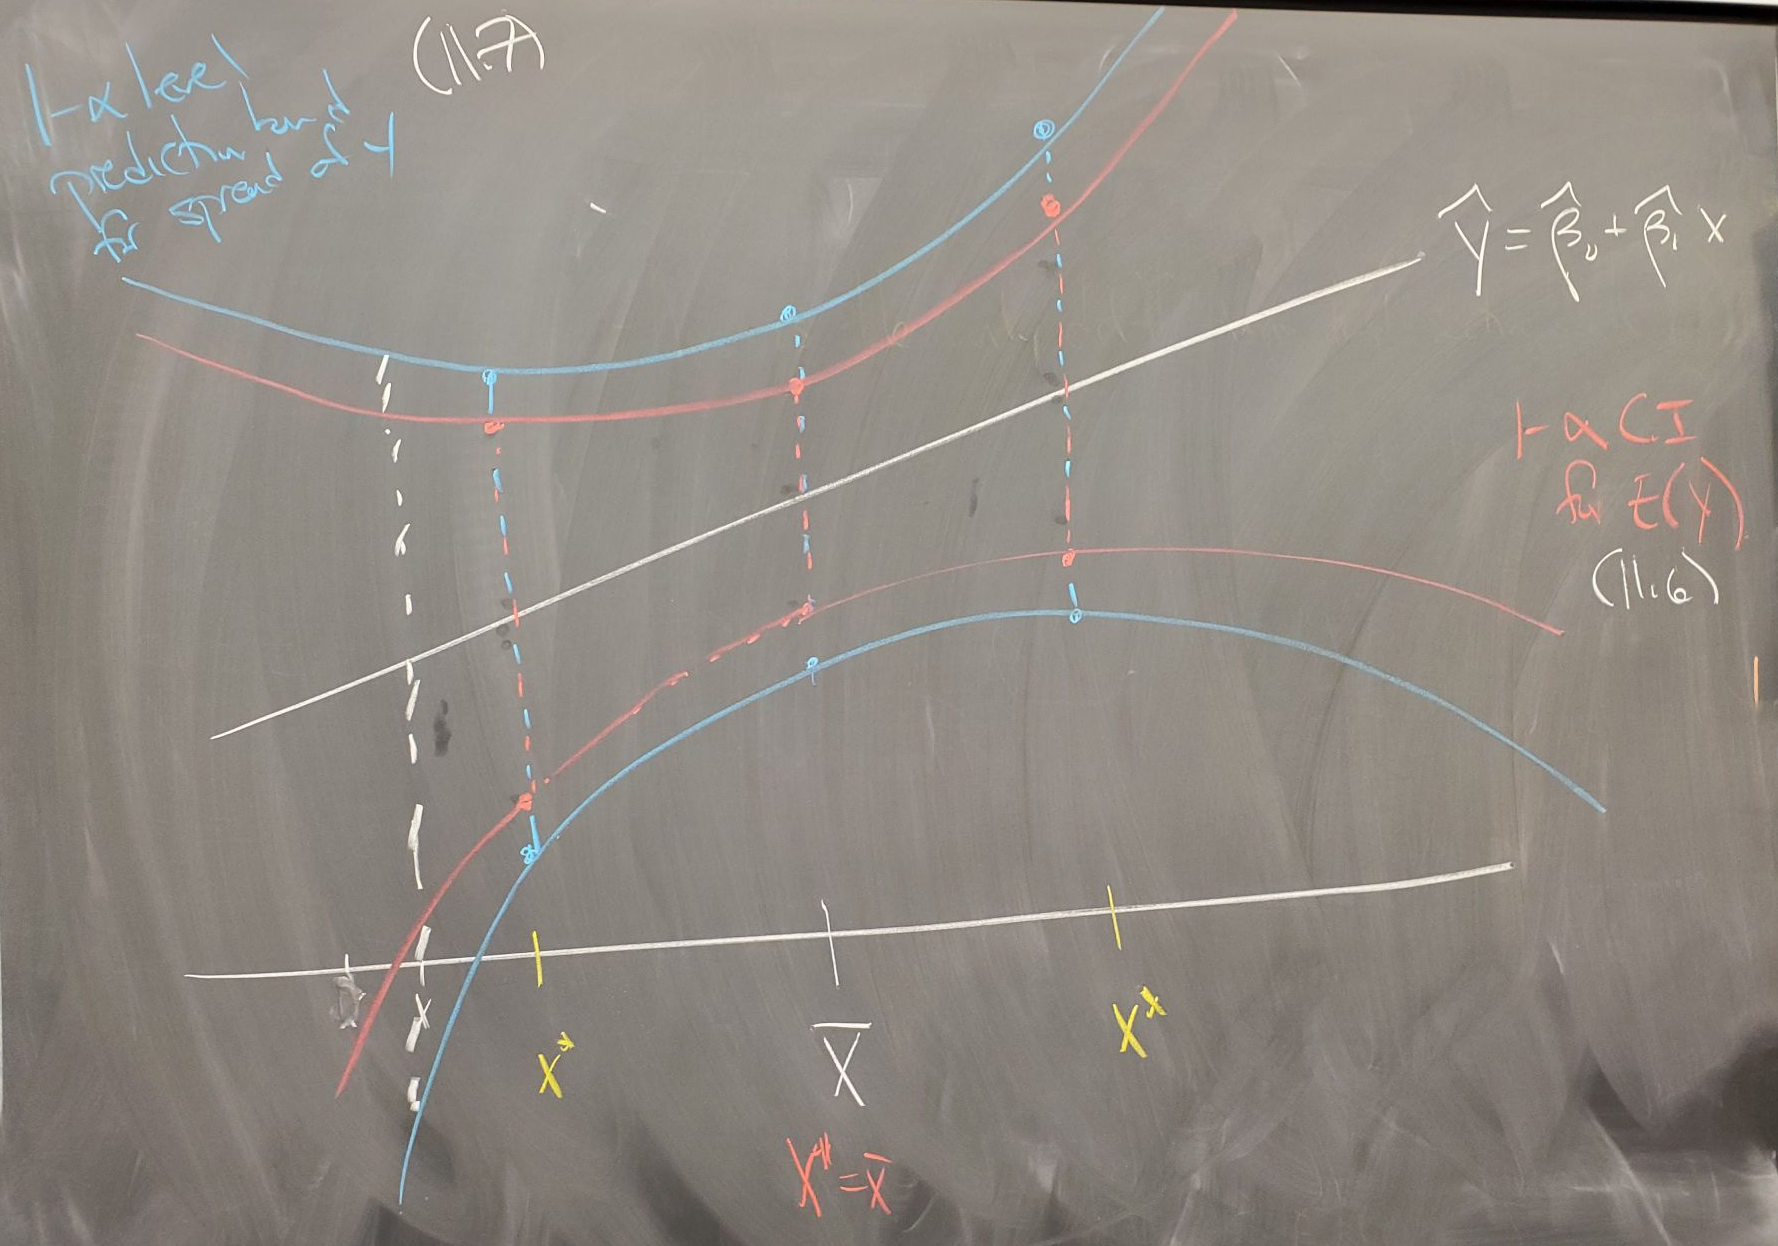
\includegraphics[width=6.5in]{11_7_hyperbola.png}
\end{center}

\noindent \textbf{Example: } Potency of antibiotic when stored at $20^{\circ}$F. Last day we showed that $\E{\widehat y(20)}$ had 90\% confidence interval
$$\setRed \underbrace{\setBlack 39.6 \pm 4.677}_{\text{red cross-section}}$$
What spread of potency would we expect to see with 90\% confidence if stored at $20^{\circ}$F. The same calculation as the last but with new standard error 
$$39.\overline6 \pm 1.812 \sqrt{1 + \over{12} + \frac{1600}{6000}}$$
$$\setBlue \underbrace{\setBlack 39.6 \pm 5.069}_{\text{blue cross-section}}$$



\setSection{9}
\section{Multiple Linear Regression}
\textbf{\color{eblue}Example: } Consider the data:
  \begin{center}
    \begin{tabular}{|l|c|c|c|c|c|} 
         \hline
         $x$ & -1 & 1 & 2 & 3\\
         \hline 
         $y$ & 0.5 & -1 & -0.5 & 2\\
         \hline
    \end{tabular}
\end{center}
The the plot does not look linear:
\begin{center}
    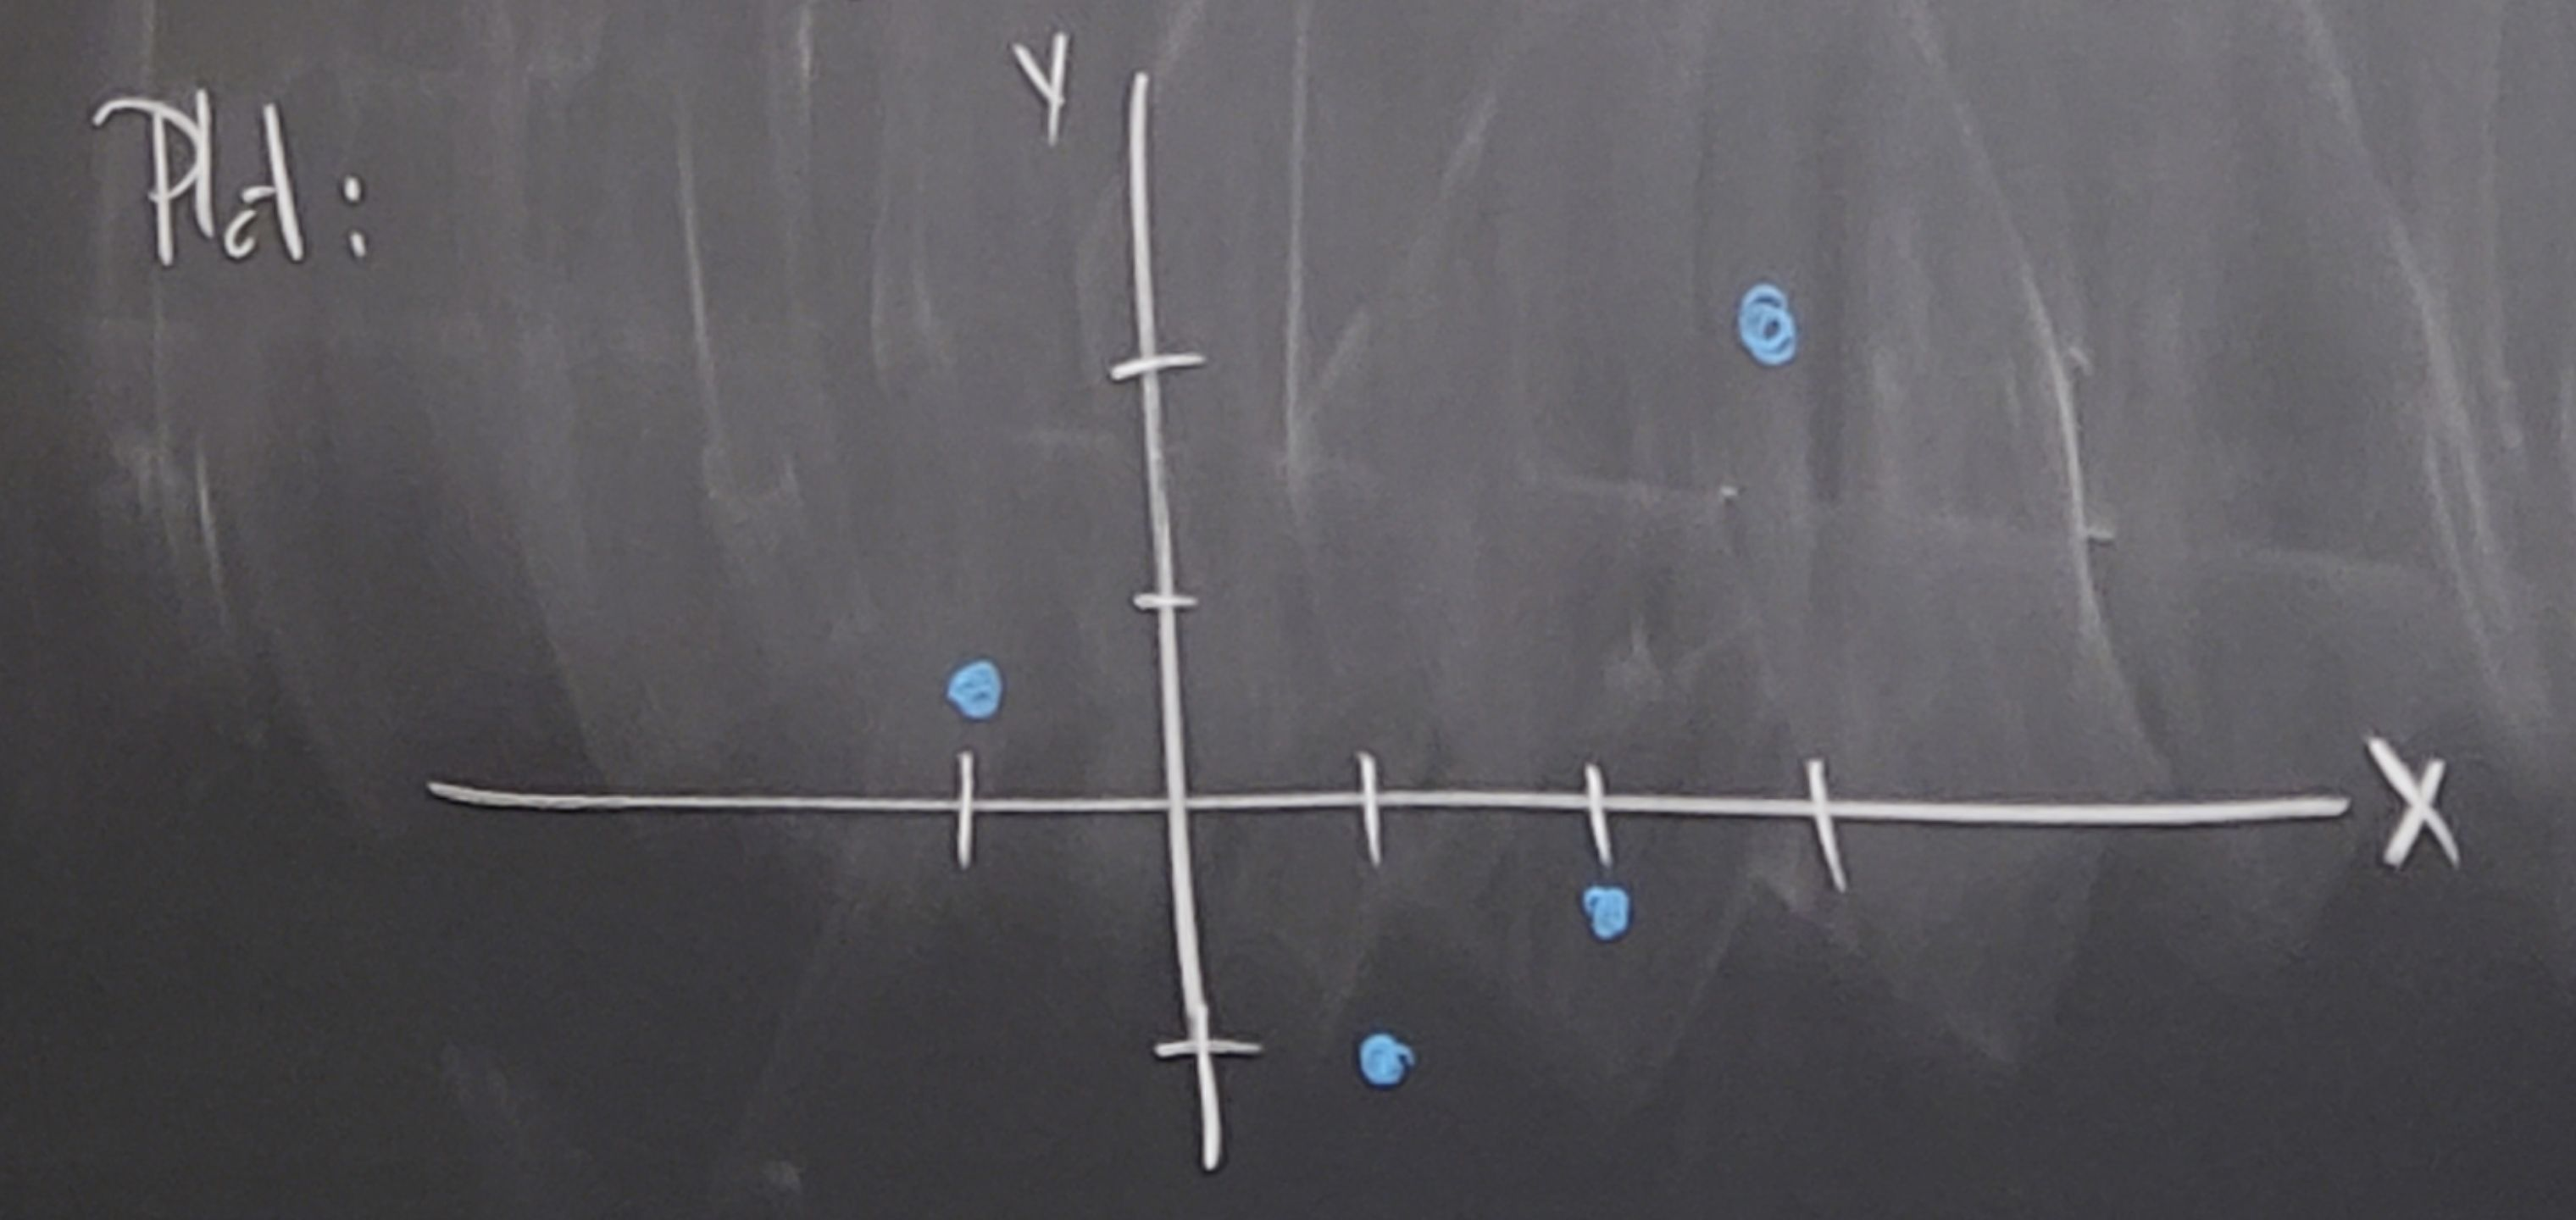
\includegraphics[height=2in]{11_10 plot.jpg}
\end{center}

\nl Seems unlikely that a line will fit well. What about a parabola? Want $y = \beta_0 + \beta_1x + \beta_2x^2$. Of course, in the probabilistic setup:
$$y = \underbrace{\beta_0 + \beta_1x + \beta_2x^2}_{\text{deterministic}} + \setRed \underbrace{ \varepsilon}_{\text{error}}$$
Using the data:
\begin{align*}
    \over{2} &= \beta_0 + \beta_1(-1) + \beta_2(-1)^2\\
    -1 &= \beta_0 + \beta_1(1) + \beta_2(1)^2 \\
    -\over{2} &= \beta_0 + \beta_1(2) + \beta_2(2)^2\\
    2 &= \beta_0 + \beta_1(3) + \beta_2(3)^2
\end{align*}
But this is the same idea as before, just in higher dimensions (3 coefficents).
$$\vec y = \beta_0 \vec 1 + \beta_1 \vec x + \beta_2 \vec{x^2}$$
$$= \beta_0 \begin{pmatrix}
    1\\1\\1\\1
\end{pmatrix} + \beta_1 \begin{pmatrix}
    -1\\1\\2\\3
\end{pmatrix} + \beta_2 \begin{pmatrix}
    1\\1\\4\\9
\end{pmatrix}$$
Or, as a matrix equation,
$$\begin{bmatrix}
    1 & -1 & 1\\ 1 & 1 & 1 \\ 1 & 2 & 4 \\ 1 & 3 & 9
\end{bmatrix} \begin{bmatrix}
    \beta_0 \\ \beta_1 \\ \beta_2
\end{bmatrix} = \begin{bmatrix}
    1/2 \\ -1 \\ -1/2 \\ 2
\end{bmatrix}.$$
Remark: This is why this process is called \textbf{linear} regression.

\nl The system for the coefficients will be a linear system. It has \red{nothing} to do with the underlying model\dots WHich here is quadratic $y = \beta_0 + \beta_1 x + \beta_2 x^2$.

\nl Just as before, we have an overdetermined system, which implies there is no solution. Hence, the best we can do is find the projection.

\nl We need a way to solve this projection problem in general. 

\nnl \textbf{Topic: The Normal Equations: }\\
In complete generality, $$y = \beta_0 + \beta_1 f_1(x) + \beta_2 f_2(x) + \cdots + \beta_n f_n(x) + \varepsilon.$$
Let there be $m$ data points $(x_i, y_i)$.

\nl This yields a matrix equation:
$$\begin{bmatrix}
    1 & f_1(x_1) & f_2(x_1) & \cdots & f_n(x_1)\\
    1 &  f_1(x_2) & f_2(x_2) & \cdots & f_n(x_2)\\
    \vdots & \vdots & \vdots & \ddots & \vdots \\
    1 &  f_1(x_n) & f_2(x_n) & \cdots & f_n(x_n)\\
\end{bmatrix} \begin{bmatrix}
    \beta_0 \\ \beta_1 \\ \vdots \\ \beta_n
\end{bmatrix} = \begin{bmatrix}
    y_1\\ y_2 \\ \vdots \\ y_n
\end{bmatrix}$$
Write $\mathbf X \vec{\beta} = \vec y$. Then $\mathbf X$ is $m$x$n$.

\nl Note, this setup really only makes sense when the system is overdetermined (more equations than unknowns). That is, more rows then columns in $\mathbf X$. i.e. $m > n$. We seek the coefficient vectors $\widehat{\beta} = [\thru{\widehat{\beta}}]$ such that $\norm{y - \mathbf X \widehat{\beta}}$ is minimized (LSR).

\nl In the gernal case, there are 2 new issues to content with:
\begin{enumerate}[label=\textcircled{\raisebox{-1pt}{\arabic*}}]
    \item no reason the column vectors of $\mathbf X$ are actually a basis for $\operatorname{Col} \mathbf X (might just be a spanning set)$.
    \item Certainly no reason columns are an orthogonal set. 
\end{enumerate}
The implication of $\textcircled{\raisebox{-1pt}{1}}$ is that a least squares solution $\widehat{\beta}$ need not be unique. As for $\textcircled{\raisebox{-1pt}{2}}$, ends we don't need this. By definition $\vec y - \mathbf X \widehat{\beta}$ is orthogonal to $\operatorname{Col}\mathbf X$.

\nl In other words, $\vec y - \mathbf X \widehat{\beta}$ must lie in the null space of $\mathbf X ^T$. (Recall $(\operatorname{Col} )^{\perp} = \operatorname{null}A^T$).

\nl Thus, $\mathbf X^T (y - \mathbf X \widehat{\beta}) = \vec 0$. 
$$\implies \underbrace{\mathbf X^T y}_{m \text{ vector}} - \underbrace{\mathbf X^T \mathbf X \widehat{\beta}}_{m \text{ vector}} = \underbrace{0}_{m}$$
$$\implies \mathbf X^T \mathbf X \widehat{\beta} = \mathbf X^T y$$
Definition: The normal equations:
$$\mathbf X^T \mathbf X \widehat{\beta} = \mathbf X^T y$$

\nl Facts:
\begin{enumerate}[label=\textcircled{\raisebox{-1pt}{\arabic*}}]
    \item $\mathbf X^T \mathbf X$ is an $n$x$n$ matrix.
    \item The normal equation is always a consistent system. That is, there is a solution to the least squares problem.
    \item If the columns of $\mathbf X$ are linearly independent, then $\mathbf X^T \mathbf X$ is an invertible square matrix and the unique solution to the least squares problem is
    $$\widehat{\beta} = \pars{\mathbf X^T \mathbf X}^{-1}\mathbf X^T y$$ 
\end{enumerate}

\example Our best fit parabola. 

$$\mathbf X = \begin{bmatrix}
    1 & -1 & 1\\ 1 & 1 & 1 \\ 1 & 2 & 4 \\ 1 & 3 & 9
\end{bmatrix}, \qquad \mathbf X^T = \begin{bmatrix}
    1 & 1 & 1 & 1\\ -1 & 1 & 2 & 3 \\ 1 & 1 & 4 & 9
\end{bmatrix}$$
$$\widehat{\beta} = [\widehat{\beta}_0, \widehat{\beta}_1, \widehat{\beta}_2], \quad y = \brac{ \over{2}, -1, -\over2, 2 }$$
$$\mathbf X^T \mathbf X = \begin{bmatrix}
    4 & 5 & 15\\ 5 & 15 & 35 \\ 15 & 35 & 99
\end{bmatrix}$$
Note that $\operatorname{det} (\mathbf X^T \mathbf X ) = 440 \neq 0$ so it is invertible. 
\begin{align*}
    \widehat{\beta} &= (\mathbf X^T \mathbf X )^{-1} \mathbf X^T y\\
    &= \begin{bmatrix}
        -41/44\\ -379/440 \\ 53/88
    \end{bmatrix}
\end{align*}
So, the best-fit parabola is 
\begin{align*}
    y &= -\frac{41}{44} - \frac{379}{440}x + \frac{53}{88}x^2\\
    &\approx -0.932 - 0.861x +0.602x^2
\end{align*}


\disc{Revisit the best-fit line}

\nl Given $n$ $(x_i,\, y_i)$'s, $y = \beta_0 + \beta_1 x + \varepsilon$. 
$$\implies \begin{bmatrix}
    \vec 1 & \bar x
\end{bmatrix} \widehat{\beta} = \vec y \wideand \widehat{\beta} = \begin{bmatrix}
    \widehat{\beta}_0\\ \widehat{\beta}_1
\end{bmatrix}$$
Here $\mathbf X = \begin{bmatrix}
    \vec 1 & \bar x
\end{bmatrix}$ is a $n\,\text{x}\,2$ matrix and $\mathbf X^T = \begin{bmatrix}
    1^T\\ x^T
\end{bmatrix}$ is $2\,\text{x}\,n$.

\nl Then
\begin{align*}
    \mathbf X^T \mathbf X &= \begin{bmatrix}
        1^T\\ x^T
    \end{bmatrix} \begin{bmatrix}
        \vec 1 & \bar x
    \end{bmatrix}\\
    &= \begin{bmatrix}
        1 \cdot 1 & 1 \cdot x\\ x \cdot 1 & x \cdot x \end{bmatrix}\\
        &= \begin{bmatrix}
            n & \sum x_i\\ \sum x_i & \sum {x_i}^2
        \end{bmatrix}
\end{align*}
Normal equation $X^TX \widehat{\beta} = X^T y$. Can we solve uniquely? 

\begin{align*}
    \det (X^TX) &= n \sum {x_i}^2 - \pars{\sum x_i}^2\\
    &= n \sum {x_i}^2 - n^2 \bar x^2\\
    &= n \pars{\sum {x_i}^2 - n \bar x}\\
    &= n S_{xx}\\
    &>0
\end{align*}
Therefore $X^TX$ is invertible! ($\det A \ne 0 \iff A^{-1}$ exists)

\nl So $\widehat{\beta} = (X^TX)^{-1}X^Ty$

\recall* $\displaystyle \begin{bmatrix}
    a & b \\ c & d
\end{bmatrix}^{-1} = \over*{\det A} \bigbrac{(\operatorname{tr}A)I - A} = \over{ad-bc} \begin{bmatrix}
    d & -b\\ -c & a
\end{bmatrix}$.

\nl So $$\displaystyle (X^TX)^{-1} = \over{nS_{xx}} \begin{bmatrix}
    \sum {x_i}^2 & - \sum x_i \\  - \sum x_i & n
\end{bmatrix} $$
and
$$X^T y = \begin{bmatrix}
    1^T \\ x^T
\end{bmatrix} y = \begin{bmatrix}
    1 \cdot y \\ x \cdot y
\end{bmatrix} = \begin{bmatrix}
    \sum y_i\\ \sum x_i y_i
\end{bmatrix}$$
Then
\begin{align*}
    \widehat{\beta} &= \over{nS_{xx}} \begin{bmatrix}
        \sum {x_i}^2 & - \sum x_i\\ -\sum x_i & n
    \end{bmatrix} \begin{bmatrix}
        \sum y_i \\ \sum x_i y_i
    \end{bmatrix}
    \\
    &= \over{n S_{xx}} \begin{bmatrix}
        (\sum {x_i}^2)(\sum y_i) - (\sum x_i)(\sum x_i y_i)\\
        -(\sum x_i)(\sum y_i) + n \sum x_i y_i
    \end{bmatrix}
\end{align*}
Same $\widehat{\beta}_0, \widehat{\beta}_1$ as earlier. But wait there's more\dots, Look at $(X^TX)^{-1}$:
\begin{align*}
    (X^TX)^{-1} &= \over{nS_{xx}} \begin{bmatrix}
        \sum {x_i}^2 & -n \bar x\\ -n \bar x & n
    \end{bmatrix}\\
    &= \begin{bmatrix}
        \dfrac{\sum {x_i}^2}{n S_{xx}} & -\dfrac{\bar x}{S_{xx}}\\ -\dfrac{\bar x}{S_{xx}} & \dfrac{1}{S_{xx}}
    \end{bmatrix}
\end{align*}
And
\begin{align*}
    \sigma^2 (X^TX)^{-1} &= \begin{bmatrix}
        \Var{\betah_0} & \Cov (\betah_0, \betah_1)
        \\ \Cov (\betah_0, \betah_1)  & \Var{\betah_1}
    \end{bmatrix}
\end{align*}
\textbf{FACT:} This always happens. $\sigma^2 (X^TX)^{-1}$ is the table of covariances:
$$\sigma^2 - a_{i\,j} = \Cov (\betah_i, \betah_j) \quad \text{where} \quad [a_{i\,j}] = (X^TX)^{-1}$$
Lastly,
$$S^2 = \frac{\operatorname{SSE}}{n-2} = \frac{\displaystyle \sum (y_i - \widehat{y}_i)^2}{n-2}$$
And \say{by some matrix algebra} (Wackerly),
$$\operatorname{SSE} = y^Ty - \betah^T \mathbf X^T y.$$

\example* (Antibiotic again)
\begin{center}
    \begin{tabular}{|l||c|c|c|c|c|c|c|c|c|c|c|c|} 
         \hline
         $x$ & 30 & 30 & 30 & 50 & 50 & 50 & 70 & 70 & 70 & 90 & 90 &90 \\
         \hline 
         $y$ & 38 & 43 & 29 & 32 & 26 & 33 & 19 & 24 & 23 & 14 & 19 & 21\\
         \hline
    \end{tabular}
\end{center}
$n = 12$ and $X^TX \displaystyle = \bmat{n}{\sum x_i}{\sum x_i}{\sum {x_i}^2} = \bmat{12}{720}{720}{\num{49200}}$. Then $\det (X^TX) = \num{72000}$. Then
$$(X^TX)^{-1} = \over{\num{72000}} \begin{bmatrix}
    \num{49200} & -700 \\ -700 & 12
\end{bmatrix}.$$
\setRed \textbf{Note:} \setBlack $\Var*{\betah_0} = \dfrac{41}{60}\sigma^2$, and $\Var*{\betah_1} = \dfrac{\sigma^2}{6000}$. 

\nl Then $X^Ty \displaystyle = \vvec*{\sum y_i}{\sum x_iy_i} = \vvec*{324}{\num{17540}}$ and $\betah = (X^TX)^{-1}X^Ty = \vvec*{46}{-19/60}$ (same as before). Hence 
$$\widehat{y} = 46 - \frac{19}{60}x$$
$$\operatorname{SSE} = y^Ty - \betah^T X^Ty = \frac{2961}{15}$$
$$\sigma^2 \approx \frac{\operatorname{SSE}}{n-2} = \frac{2971/15}{10} \approx 19.8067.$$
\section{A big ol theorem}

\nl Theorem: Let $Y_i = \beta_0 + \beta_1 f_1(x_i) + \cdots + \beta_k f_k (x_i) + \varepsilon_i$ where $\varepsilon_i \sim \normalDist{0, \sigma^2}$ (with $\Eb{\varepsilon} = 0$).

\nl Then the least-squares estimates are given by $\widehat{\beta} = (X^TX)^{-1}X^Ty$ provided $(X^TX)^{-1}$ exists. Then 

\begin{enumerate}[label=\textcircled{\raisebox{-1pt}{\arabic*}}]
    \item $\E*{\betah_i} = \betah_i \qquad \text{(unbiased)}$
    \item $\Var*{\betah_1} = c_{i\,i} \sigma^2$ \hspace{.2in} where $(X^TX)^{-1} = [c_{i\,j}]$
    \item $\Cov(\betah_i, \betah_j) = c_{i\,j} \sigma^2$
    \item $S^2 = \dfrac{\operatorname{SSE}}{n-(k+1)}$ \hspace{.1in} with $k+1 \; \betah_i$'s and $\operatorname{SSE} = y^Ty - \betah^T X^Ty$ and $\E{S^2} = \sigma^2$ (unbiased)
    \item $\betah_i$ is normally distributed.
    \item $\dfrac{(n-(k+1))S^2}{\sigma^2} \sim \chi^2(n-(k+1))$
    \item $S^2$ and $\betah_1$ are independent for all $i$.
\end{enumerate}
\section{Hypothesis Testing C.I.}
Motivation: Testing a specific $\betah_i$.

\nl We have $\betah = (X^TX)^{-1}Ty = [\betah_0, \dots, \betah_k]$. To pick off a specific $\betah_i$, we use the dot product.

\nl Let $e_i$ (standard basis vector), then $\displaystyle \betah_i = \underbrace{e_i \cdot \betah}_{\text{dot product}} = \underbrace{{e_i}^T \betah}_{\substack{\text{matrix} \\ \text{multiplication}}}$

\nl Note: $\E*{e_i \cdot \betah} = \E*{1 \cdot \betah_i} = \E*{\betah_i} = \beta_i$.
\\ Same with $\Var*{e_i \cdot \betah} = \Var*{\betah_i}$.

\nl So a test of the form
\begin{align*}
    H_0 &: \betah_i = (\beta_i)_0\\
    H_a &: \betah_i \neq (\beta_i)_0
\end{align*}
yields same old statistics.
$$Z = \frac{\betah_i - (\beta_i)_0}{\sqrt{\Var*{\beta_i}}} = \frac{\betah_i - (\beta_i)_0}{\sqrt{c_{i\,i}\sigma^2}} \qquad \text{with} \qquad [c_{i\,i}] = (X^TX)^{-1}$$
$$T = \frac{\betah_i - (\beta_i)_0}{S \sqrt{c_{i\,i}}} \qquad \text{with} \qquad n-(k+1) \text{ df.}$$

\example*
We fit
\begin{center}
    \begin{tabular}{|l|c|c|c|c|c|}
         \hline
         $x$ & -1 & 1 & 2 & 3\\
         \hline
         $y$ & 0.5 & -1 & -0.5 & 2\\
         \hline
    \end{tabular}
\end{center}
with $y = \beta_0 + \beta_1 x + \beta_2 x^2$ because it \say{looked} non-linear.
\begin{center}
    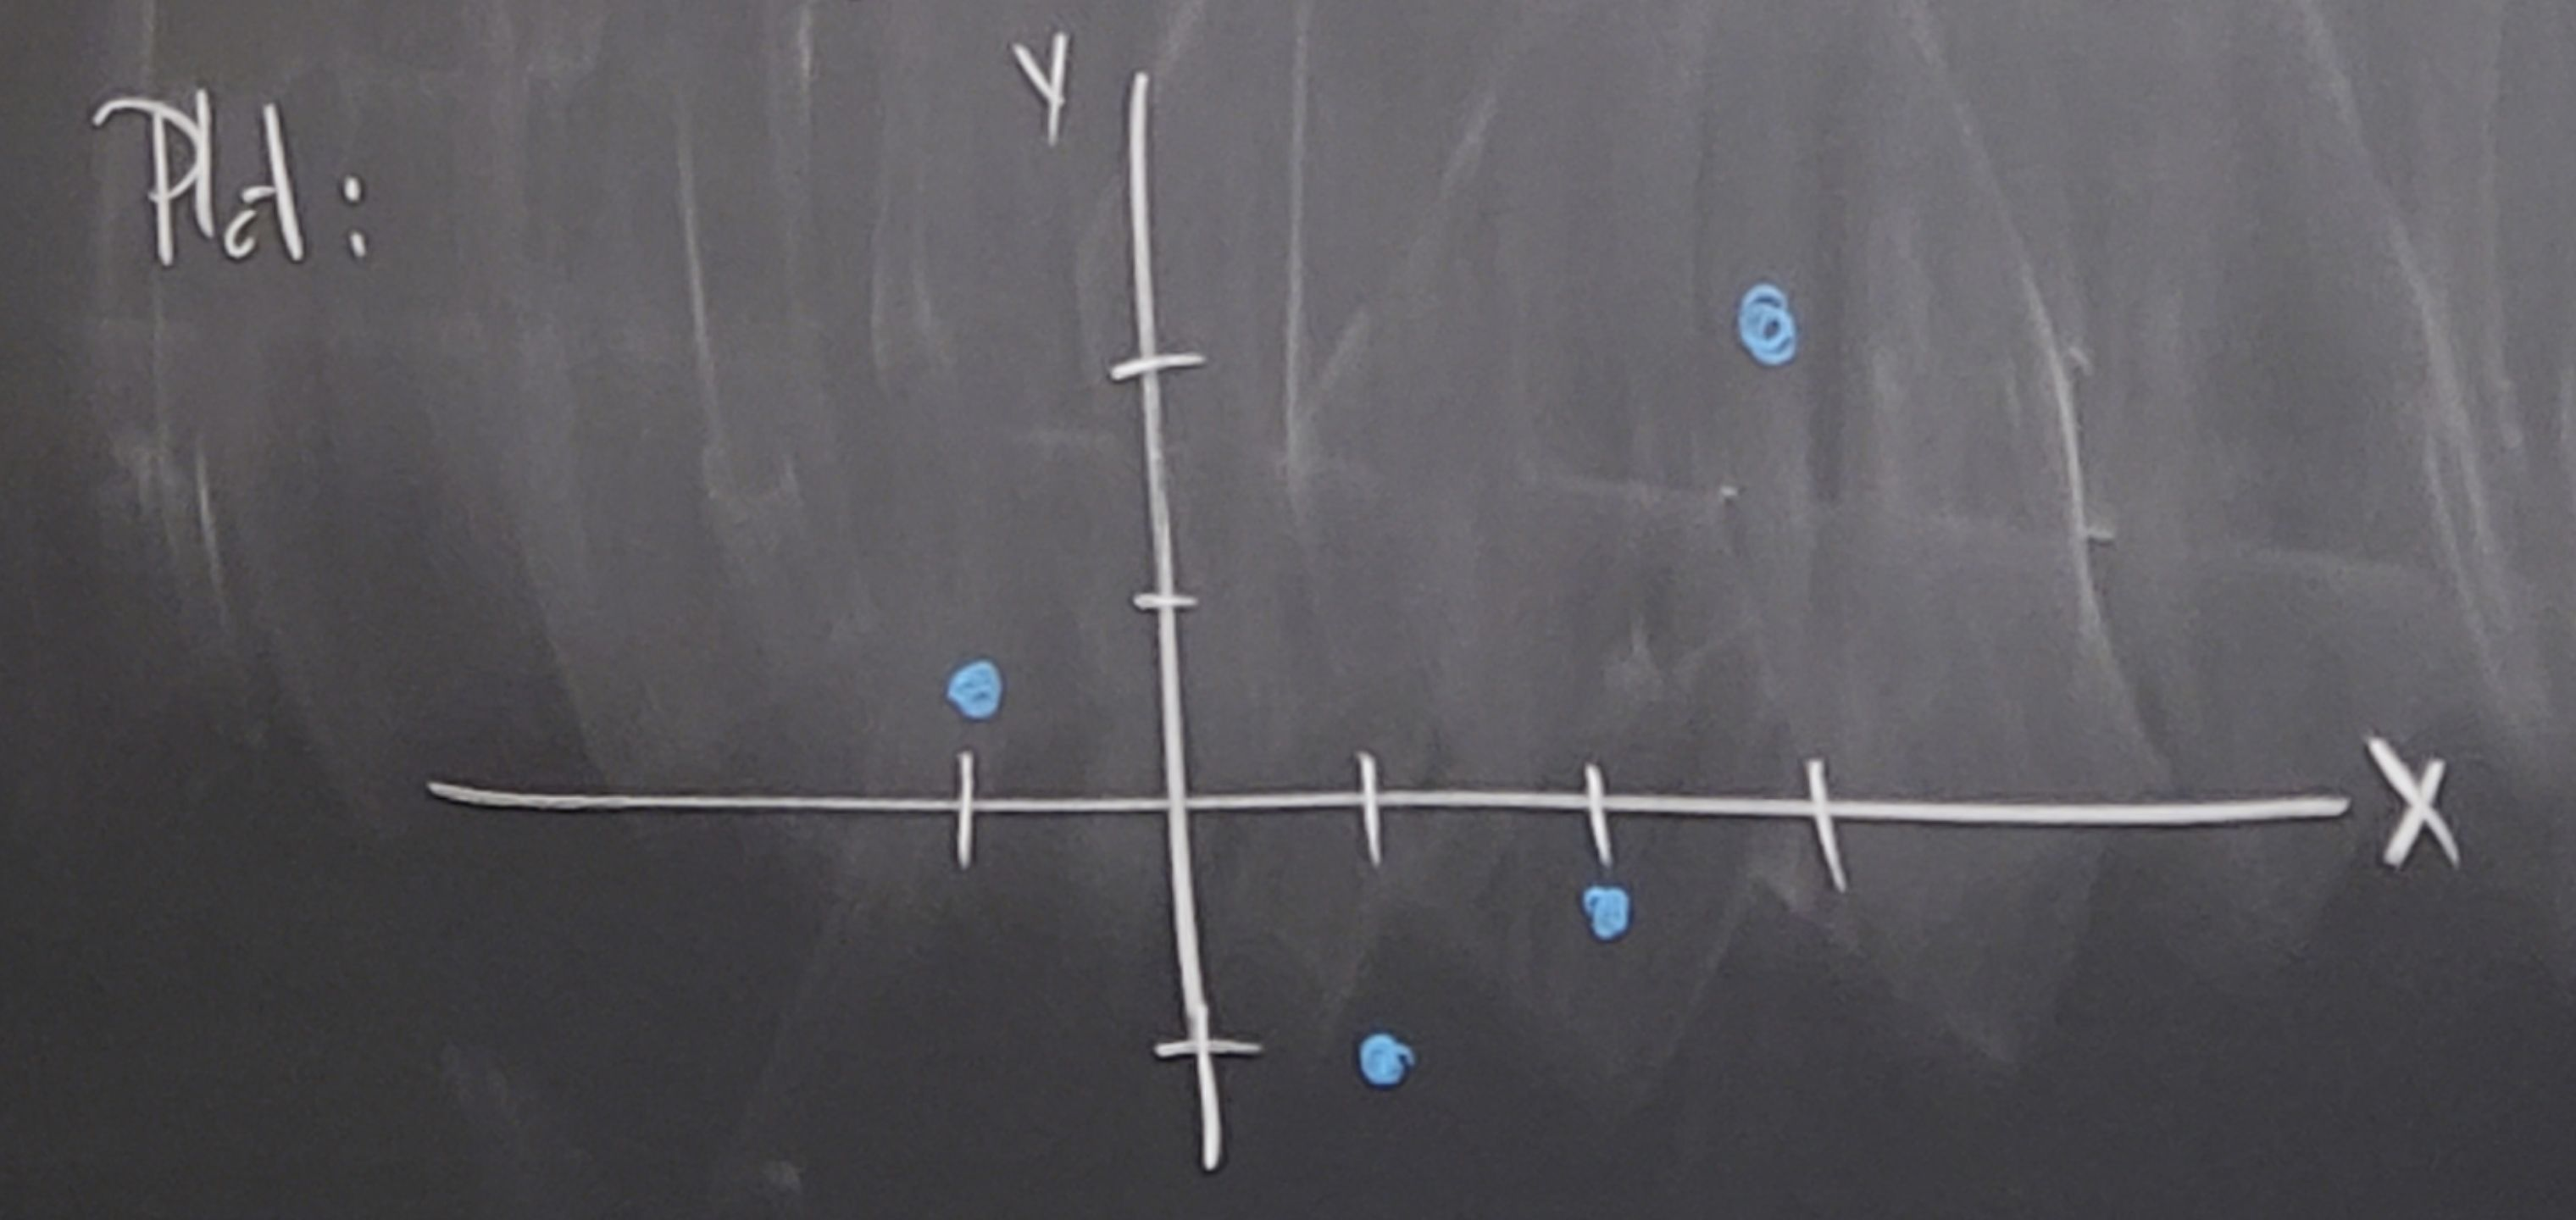
\includegraphics[height=2in]{11_10 plot.jpg}
\end{center}
Is there evidence that the data is in fact non-linear? That is, are we reasonably certain $\beta_{\alpha} \neq 0$.
\begin{align*}
    H_0 &: \beta_{\alpha} = 0\\
    H_a &: \beta_{\alpha} \neq 0
\end{align*}
We had
\begin{align*}
    \widehat{\beta} &= (\mathbf X^T \mathbf X )^{-1} \mathbf X^T y\\
    &= \begin{bmatrix}
        -41/44\\ -379/440 \\ 53/88
    \end{bmatrix}\\
    &= \vvec*{\betah_0}{\betah_1}{\betah_2}
\end{align*}
$e_3 = (0,0,1)$ and ${e_3}^T\betah = \dfrac{53}{80}$. We had
$$\mathbf X^T \mathbf X = \begin{bmatrix}
    4 & 5 & 15\\ 5 & 15 & 35 \\ 15 & 35 & 99
\end{bmatrix}$$
and $\det (\mathbf X^T \mathbf X) = 440$. Then
$$(\mathbf X^T \mathbf X)^{-1} = \over{440} \begin{bmatrix}
    260 & 30 & -50 \\
    30 & 171 & -65\\
    -50 & -65 & 35
\end{bmatrix}$$
With $\Var*{\betah_2} = c_{2\,2} \sigma^2 = \dfrac{35}{440}\sigma^2$. % was this beta2?

\nl For $\sigma^2$, we need $S^2 = \dfrac{\operatorname{SSE}}{n-2}$.
$$\operatorname{SSE} = y^Ty - \betah^T X^Ty = \frac{4791}{440}.$$
$$S^2 = \frac{\frac{4791}{440}}{n-2} = \frac{4791}{850} \approx 5.44432.$$
$$\Var*{\betah_2} \approx c_{2\,2} S^2 \cdots \sqrt{\Var*{\betah_2}} = 0.690201.$$
So
\begin{align*}
    T &= \frac{e_3 \cdot \betah - (\betah_2)_0}{\sqrt{\Var*{\betah_2}}}\\
    &= \frac{\frac{53}{88}-0}{0.690201}\\
    &= 0.872604
\end{align*}
$$\P{\abs{T} \geq 0.872604 \mid \df = 2} = 0.4748909.$$
\red{This sucks! It supports the null Hypothesis.}

\example* (Potency again)
\begin{center}
    \begin{tabular}{|l||c|c|c|c|c|c|c|c|c|c|c|c|}
         \hline
         $x$ & 30 & 30 & 30 & 50 & 50 & 50 & 70 & 70 & 70 & 90 & 90 &90 \\
         \hline
         $y$ & 38 & 43 & 29 & 32 & 26 & 33 & 19 & 24 & 23 & 14 & 19 & 21\\
         \hline
    \end{tabular}
\end{center}
I tried quadratic $y = \beta_0 + \beta_1x + \beta_2x^2$.
$$X = \begin{bmatrix}
    1 & x & x^2
\end{bmatrix}$$
$$(X^TX)^{-1} = \over{1.92 \times 10^6} \begin{bmatrix}
    1.092 \times 10^6 & -391200 & 3100\\
    -391200 & 14720 & -120\\
    3100 & -120 & 1
\end{bmatrix}$$
Note: $\Var*{\betah_2} = \over*{1.92 \times 10^6}\sigma^2 \approx \dfrac{S^2}{1920000}$.
$$\operatorname{SSE} = y^Ty + \betah^TX^Ty = 189.$$
$$S^2 = \frac{\operatorname{SSE}}{n-2} = \frac{\operatorname{SSE}}{10} = 18.9$$
$$\Var*{\betah_2} = 9.84775 \times 10^{-6}.$$
$$\sqrt{\Var*{\betah_2}} = 0.00313748$$
Testing
\begin{align*}
    H_0 &: \beta_2 = 0\\
    H_a &: \beta_2 \neq 0
\end{align*}
I computed $\betah_2 = \over*{1200}$.
$$t = \frac{\betah_2 - (\beta_2)_0}{\sqrt{\Var*{\betah_2}}} = 0.2656$$
With $\df = 10$, $\P{\abs{T} > 0.2656} = 0.79$, which is HUGE again. Hence it supports the null hypothesis.

\nl Of course, this is a math class and we love to generalive. We don't have to use a standard basis vector $e_i$. Let $\vec{a}$ be a constant vector $a = (a_0, \dots, a_k)$. Then
$$a^T\betah = a_0 \betah_0 + \dots + a_k \betah_k.$$
Note:
\begin{align*}
    \E*{a^T \betah} &= \sum{i=1}^k a_i \E*{\betah_i} \tag{by linearity}\\
    &= \sum{i=1}^k a_i \beta_i \tag{by unbiases estimators}\\
    &= a^T \beta
\end{align*}
for $\beta = (\beta_0, \dots, \beta_k)$. Also,
\begin{align*}
    \Var*{a^T \betah} &= \Var*{a_0 \betah_0 + \cdots + a_k \betah_k}\\
    &= \sum{i=1}^k \sum{j=1}^k \Cov (a_i \betah_i, a_j \betah_j)\\
    &= \sum{i=1}^k \sum{j=1}^k a_i a_j \underbrace{\Cov (\betah_i, \betah_j)}_{\substack{\text{These are } c_{i\,j} \sigma^2 \text{'s} \\ \text{from } (X^TX)^{-1}}}
\end{align*}
This entire double sum can be written as the matrix product
$$\Var*{a^T \betah} = a^T (X^TX)^{-1}a \cdot \sigma^2$$
% = 1xk, kxk, kx1
$$\implies Z = \frac{a^T \betah - \E{a^T \betah}}{\Var{a^T\betah}} = \frac{a^T \betah - a^T \beta}{\sigma \sqrt{a^T (X^TX)^{-1} a} }$$

\nl Given $H_0 : a^T \beta = (a^T \beta)_0$ versus some alternative, use
$$T = \frac{a^T \betah - (a^T \beta)_0}{S \sqrt{a^T (X^TX)^{-1}a}}$$
with $n-(k+1)$ degrees of freedom. 
\setChapter{12}
\chapter{One-way Analysis of Variance}
We know how to test fit the difference in 2 means
\begin{align*}
    H_0 &: \mu_1 = \mu_2 \qquad \text{i.e} \qquad \mu_1 - \mu_2 = 0.\\
    H_a &: \mu_1 \neq \mu_2  \qquad \text{i.e} \qquad \mu_1 - \mu_2 \neq 0
\end{align*}
Now we endeavor to construct a test to detect difference in means over multiple groups.

\example* 24 expert typists test three new keyboard designs. Randomly assign 8 to each type of keyboard and assigned the same document to type up. The time of the task is recorded with the idea that a group with significantly less time on task would imply a better keyboard design
  \begin{center}
    \begin{tabular}{|c|c|}
         \hline
         design & times\\
         \hline
         KB1 & 364 366 394 386 379 398 371 370\\
         KB2 & 355 359 374 342 378 355 376 358\\
         KB3 & 360 345 374 390 386 373 393 366\\
         \hline
    \end{tabular}
\end{center}
An obvious stat to look at is means
$$\bar{A} = 378.5 \qquad \bar{B} = 362.125 \qquad \bar{C} = 373.375$$
$B$ \say{looks} better, but can we design a test to determine if it is \say{significantly} so? This is our goal.

\nl The standard null hypothesis is that the true population means are the same for each group, $H_0: \mu_1 = \mu_2 = \cdots = \mu_k = \mu_0$. The alternative $H_a$ is that at least one of the $\mu_i$'s are different.

\nl Notation: Let $i$ indicate the \say{group}. E.g. $k_i$ with $i = 1, 2, 3$. ($k$ for keyboard). Let $j$ denote the data point in that group. i.e. $Y_{1\,3} = 394$, $Y_{2\,5} = 378$.

\nl Let $n_i$ be the number of data points in the $i^{\text{th}}$ group. Here $n_1 = n_2 = n_3 = 8$. Let $n$ be the total of all data points. $n = \sum_{i=1}^k n_i$. Here $n = 24$.

\nl Formally, we assume $Y_{i\,j} \sim N(\mu_i, \sigma^2)$ where each group has mean $\mu_i$, but all groups have the same variance $\sigma^2$.
\\We need a stat.

\nl To find \say{a} stat, we construct a likelihood ratio test. For $H_0$ we have our usual MLEs. If there is only $\mu_0$
$$\muh_0 = \over{n} \sum_{i=1}^k \sum_{j=1}^{n_i} Y_{i\,j}$$
and $${S_0}^2 = \sum_{i=1}^k \sum_{j=1}^{n_i} (Y_{i\,j} - \muh_0)^2.$$
Under the alternative hypothesis, for the individual means, we again use the standard MLE
$$\muh_i = \over{n_i}\sum_{j=1}^{n_i} Y_{i\,j} = \bar{Y_i}.$$
Aside: In our motivational example, $\bar{A} = \bar{Y_1} = 378.5$, $\bar{B} = \bar{Y_2} = 362.125$, etc.

\nl But we are still assuming a unique $\sigma^2$ for all groups. So the MLE for $$S_a^2 = \over{n} \sum_{i=1}^k \sum_{j=1}^{n_i} (Y_{i\,j} - \muh_i)^2.$$
Remark: Proving that this is an MLE is a good review and will be coming to a homework soon.

\nl Construct a likelihood function:
\begin{align*}
    L(\text{All } Y_{i\,j} \mid \muh_0, S_0^2) &= \prod_{i=1}^k \prod_{j=1}^{n_i} \pover{2\pi S_0^2}^{1/2} \exp \pfrac{-(Y_{i\,j - \muh_0})^2}{2S_0^2}\\
    &= \pover{2\pi S_0^2}^{n/2} \exp \pars{- \over{2S_0^2} \sum_{i=1}^k \underbrace{\sum_{j=1}^{n_i} (Y_{i\,j} - \muh_0)^2}_{\textstyle nS_0^2}}\\
    &= \pover{2\pi S_0^2}^{n/2} \exp \pars{- \frac{nS_0^2}{2S_0^2}}\\
    &= \pover{2\pi S_0^2}^{n/2} e^{-n/2}
\end{align*}
Under $H_a$, same \say{algebra} occurs.
$$L(\text{All } Y_{i\,j} \mid \muh_0, S_a^2) =  \pover{2\pi S_a^2}^{n/2} e^{-n/2}$$
Then the ratio of likelihood functions yields
$$\frac{
    L(\text{All } Y_{i\,j} \mid H_0)
}{
    L(\text{All } Y_{i\,j} \mid H_a)
} = \frac{
    \pover{2\pi S_0^2}^{n/2} e^{-n/2}
}{
    \pover{2\pi S_a^2}^{n/2} e^{-n/2}
} = \pfrac{S_a^2}{S_0^2}^{n/2} < k$$
Implies the statistic $T = \dfrac{S_a^2}{S_0^2}$ and small values of $T$ support the alternative hypothesis (define our RR). This makes sense because if the true means are different then $S_a^2$ will be the correct estimator for $\sigma^2$ and $S_0^2$ will be larger (on average).

\nl We have a problem\dots This is an entirely new stat for us.

\nl One thing we should show is that (a)
$$S_a^2 \text{ is an estimator of } \sigma^2$$
moreover, we need it unbiased.

\nl Note that via multiplying by the correct degrees of freedom $\nu$, and dividing by $\sigma^2$, the numerator and denominator are $\chi^2$ distributed. This lead to the advent of the $F$-distribution.

\nnl Topic: The $F$-distribution. Suppose $X_1 \sim \chi^2(m)$ and $X_2 \sim X^2(n)$ and are independent. Define
$$Y_i := \frac{X_1\big/  m}{X_2 \big/ n}$$
to be an $F$ random variable with $m$ numerator degrees of freedom and $n$ denominator degrees of freedom. We usually write $Y_i \sim F(m,n)$.

\nl The derivation is akin to the derivation of the $T$-stat. We used the Jacobian method of transformations. ($\S6.6$ in the text. This is usually skipped in MTH 325.)

\nl Letting $Y_2 = X_2$, we can find the joint density function of $Y_1$ and $Y_2$, then we integrate the joint density to get the marginal density of $Y_i$\dots
$$
    f(y_1) = \dfrac{
        \Gamma \pfrac*{m+n}{n}
    }{
        \Gamma \pfrac*{m}{2} \Gamma \pfrac*{n}{2}
    } \pfrac{m}{n}^{n/2}
    \frac{
        y_1^{m/2 -1}
    }
    {
        \pars{1 + \pfrac*{my_1}{n}^{(m+n)/2}}
    } \text{ and } y_i > 0.
$$

%"last day" picture
\nl \textbf{Last day:} Looking at at designing a test $H_0 : \mu_1 = \mu_2 = \cdots = \mu_k = \mu_0$ versus $H_a$ not all equal.

\nl Theorem: Likelihood ration, find a new (for us) statistic that looked like a $\dfrac{\chi^2 \text{ r.v.}}{\chi^2 \text{ r.v.}}$. This lead us to the $F$-distribution.

$$Y \sim F(m,n) \qquad \text{when} \qquad Y = \frac{X_1/m}{X_2/n}$$
and
$$X_1 \sim \chi^2(m) \wideand X_2 \sim \chi^2(n).$$
Graph $f(y), y >0$:
\notab{
    \begin{center}
        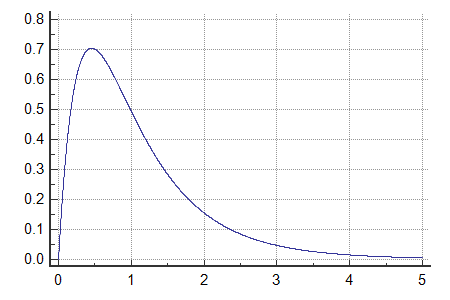
\includegraphics[width=3in]{F_graph.png}
    \end{center}
}

\nl For $\E{Y}$ and $\Var{Y}$.
\begin{align*}
    \E{Y} &= \E{ \frac{X_1/m}{X_2/n}}\\
    &= \E{\frac{n}{m}\cdot \frac{X_1}{X_2}}\\
    &= \frac{n}{m} \E{X_1 \cdot \over{X_2}}\\
    &= \frac{n}{m} \E{X_1} \E{\over{X_2}} \tag{by independence}\\
    &= \frac{n}{m} \cdot m \E{\over{X_2}}\\
    &= n \E{\over{X_2}} \tag{numerator df has no impact}\\
    &= n \cdot \underbrace{\over{n-2}}_{\text{by thm.}}
\end{align*}
$$\E{Y} = \frac{n}{n-2}.$$
Also, with proof omitted,
$$\Var{Y} = \frac{2n^2 (m+n-2)}{n(n-2)^2(n-4)}.$$
End $F$-distribution background. Then,
$$T = \frac{{S_0}^2}{{S_a}^2} = \frac{
    \over{n} \sum_{i=1}^k \sum_{j=1}^{n_i} (Y_{i\,j} - \muh_0)^2
}{  \over{n} \sum_{i=1}^k \sum_{j=1}^{n_i} (Y_{i\,j} - \muh_i)^2}$$
and the $\over{n}$ can cancel. If $S_0^2$ and $S_a^2$ were independent, then dividing by their degrees of freedom would yield an $F$-distribution. Sadly, they aren't. But we can algebra to independent ratios. Start with the top,
\begin{align*}
    {S_0}^2 &=  \sum_{i=1}^k\sum_{j=1}^{n_i} (Y_{i\,j} - \muh_0)^2\\
    &= \sum_{i=1}^k \sum_{j=1}^{n_i} \pars{(Y_{i\,j} - \muh_i) + (\muh_i - \muh_0)}^2\\
    &= \sum_{i=1}^k \sum_{j=1}^{n_i} \brac {
        (Y_{i\,j} - \muh_i)^2 + 2(Y_{i\,j- \muh_i})(\muh_i - \muh_0) + (\muh_i - \muh_0)^2
    }\\
    &=  \sum_{i=1}^k \sum_{j=1}^{n_i} (Y_{i\,j} - \muh_i)^2 + 2 \sum_{i=1}^k \bigbrac{
        (\muh_i - \muh_0) \underbrace{
            (Y_{i\,j} - \muh_i)
        }_{
            \substack{= 0\text{ as it's the} \\ \text{sum of all} \\ \text{deviations for} \\ \text{mean within a} \\ \text{group from group mean}}
        }
    } + \sum_{i=1}^k n_i( \muh_i - \muh_0 )^2\\
    &= \sum_{i=1}^k \sum_{j=1}^{n_i} (Y_{i\,j} - \muh_i)^2 + \sum_{i=1}^k n_i( \muh_i - \muh_0 )^2\\
    &= {S_a}^2 +  \sum_{i=1}^k n_i( \muh_i - \muh_0 )^2
\end{align*}
Then
$$\frac{{S_0}^2}{{S_a}^2} = 1 + \frac{
    \sum_{i=1}^k n_i (\muh_i - \muh_0)^2
}{
    \sum_{i=1}^k \sum_{j=1}^{n_i} (Y_{i\,j} - \muh_i)^2
}$$
We are pretty close to independence. Recall we have Fisher's Theorem:
 $\chi^2 \sim N(\mu, \sigma^2)$ then $\Xbar$ and $S^2$ are independent random variables and $\Xbar \sim N(\mu, \sigma^2/n).$
 $$(n-1)\frac{S^2}{\sigma^2} \sim \chi(1)$$
Thus the $\muh_i$'s up top are independent of all the variances ${S_i}^2$ in sum of the denominator. Also, $\muh_0$ \underline{is} a function of $\muh_i$
$$\muh_0 = \frac{
    n_1 \muh_1 + n_2 \muh_2 + \cdots + n_k \muh_k
}{n}$$
And the entire numerator is independent of the variance terms in the numerator when $H_0$ is true. Now, when $H_0$ is true, all the resultant variable (top and bottom) are $\chi^2$ distributed. The last thing to do is figure out degrees of freedom. Given $\mu_0$,
$$\frac{\muh_1 - \mu_0}{\sigma / \sqrt{n_i}} \sim N(0,1) \wideand \frac{n_i(\muh_i - \mu_0)^2}{\sigma^2} \sim \chi^2(1)$$
So, the sum of $\chi^2$ random variables is also a $\chi^2$ rv and the degrees of freedom add. Thus
$$\over{\sigma^2} \sum_{i=1}^k n_i (\muh_i - \mu_0)^2 \sim \chi^2(k).$$
On the other hand, to use these facts, use the say \say{trick} again
$$\muh_1 - \mu_0 = \red{(} \muh_1 - \muh_0 \red{)} + \red{(} \muh_0 - \mu_0 \red{)}$$
And
$$\sum_{i=1}^k n_i (\muh_i - \mu_0)^2 = \underbrace{
\sum_{i=1}^k n_i (\muh_i - \muh_0)^2
}_{
    \text{the numerator}
} + n \underbrace{
    (\muh_0 - \mu_0)^2
}_{
    \substack{\text{divide by } \sigma^2, \\ \text{this is } \chi^2(1)}
}$$
In the end
$$\underbrace{
    \over{\sigma^2} \sum_{i=1}^k n_i (\muh_i - \mu_0)^2
}_{\textstyle \chi^2(k)} = \underbrace{
    \over{\sigma^2}  \sum_{i=1}^k n_i (\muh_i - \muh_0)^2
}_{
    \substack{\text{the numerator is} \\ \textstyle \chi^2(k-1)}
} + \underbrace{
    n\frac{ (\muh_0 - \mu_0)^2}{\sigma^2}
}_{\textstyle \chi^2(1)}$$
Denominator is much easier,
$$\sum_{i=1}^k \underbrace{\sum_{j=1}^{n_i} \frac{(Y_{i\,j} - \mu_i)^2}{\sigma^2}}_{\textstyle {S_i}^2 \sim \chi^2(n_i - 1)}$$
and by independences, summing all the $\chi^2(n_i -1)$ variables yield a
$$\chi^2 \underbrace{\pars{\sum_{i=1}^k (n_i - 1)}}_{\text{add all \df}} = \chi^2(n-k)$$
This is a ton of work, but in the end we have
$$F = \frac{
    \sum_{i=1}^k n_i (\muh_i - \mu_0)^2 \Big/ k-1
} {
    \sum_{i=1}^k \sum_{j=1}^{n_i} (Y_{i\,j} - \muh_i)^2 \Big/ n-k
} \sim F(k-1,\, n-k)$$
when $H_0$ is true.

\nl Topic: The ANOVA test.
\begin{enumerate}[label=\textcircled{\raisebox{-1pt}{\arabic*}}]
    \item Compute the null and alternative estimate of all the sample means.
    \item Use these to compute the sum of squares in our $F$-statistic
    \item Construct a table (R or Excel?) to compute the $p$-value.\\$F_{\text{obs}}$ is $F$ observed. We computed this.
    $$\P{F > F_{\text{obs}}},\; F - F(k-1,n-k)$$
    \notab{
    \begin{center}
        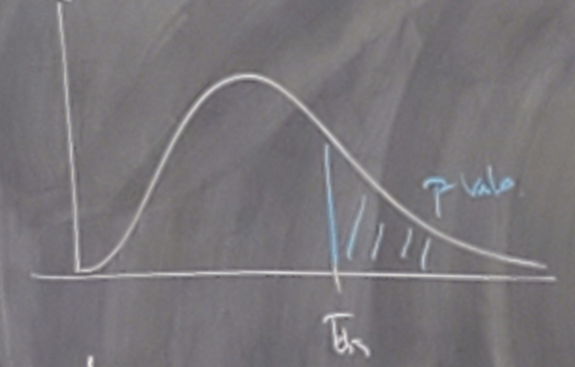
\includegraphics[width=3in]{upperTail_F.png}
    \end{center}
}
    \item Conclusion. There is standard language for all this. In the denominator,
    $$\SSW = \sum_{i=1}^k \sum_{j=1}^{n_i} (Y_{i\,j} - \muh_i)^2$$
    the sum of squares \underline{WITHIN} a group. And the numerator
    $$\SSA = \sum_{i=1}^k n_i (\muh_i - \mu_0)^2$$
    the sum of the squares \underline{AMONG} groups. A measure of variance among the sample means. Recall originally,
    $$\frac{{S_0}^2}{{S_a}^2} = \frac{{S_a}^2 + \SSA}{\SSW}$$
    Thus we showed the factorization yield \underline{total variation}.
    $$S_{0}^2 = \SSW + \SSA \qquad \text{or} \qquad \SST = \SSW + \SSA$$
\end{enumerate}

%F observed = Fobs start of 4/22
\nnl ANOVA Test
$$\SSA = \sum_{i=1}^k n_i (\muh_1 - \muh_0)^2 \qquad \text{(SS among groups)}$$
$$\SSW = \sum_{i=1}^k \sum_{j=1}^{n_i} (Y_{i\,j} - \muh_i)^2 \qquad \text{SS within groups}$$
$${S_0}^2 = \SST = \SSA + \SSW$$
$$R^2 = \frac{\SSA}{\SST} \quad \text{coef. of determination}$$

\nl Discussion: The ANOVA table
% Source | SS  |  df | MS      | F_obs   | p value
% -------+-----+-----+---------+---------+
% among  | SSA | k-1 SSA/(k-1) | MSA/MSW | P(F(k-1,n-k)>F_obs)
% within | SSW | n-k SSW/(n-k) |
% total  | SST | n-1

  \begin{center}
    \begin{tabular}{|l|c c c c c|}
         \hline
         Source & SS & df & Mean Squares & $F_{\text{obs}}$ & $p$-value\\
         \hline
         among & $\SSA$ & $k-1$ & $\SSA/(k-1)$ & $\operatorname{MSA}/\operatorname{MSW}$ & $\P{F(k-1, n-k) > F_{\text{obs}}}$ \\
         within & $\SSW$ & $n-k$ & $\SSW/(n-k)$ & & \\
         total & $\SST$ & $n-1$ & & &\\
         \hline
    \end{tabular}
\end{center}

\example*
\begin{center}
    \begin{tabular}{|l|c c c|}
         \hline
         Treatment & & Data & \\
         \hline
         1 & 2 & 4 & 3 \\ 2 & 6 & 4 & \\ 3 & 3 & 5 & 4\\
         \hline
    \end{tabular}
\end{center}
Mean squares $k=3, n_1 = 3, n_2 = 2, n_3 = 3, n = 8, \muh_1 = 3, \muh_2 = 5, \muh_3 = 4$.
$$\muh_0 = \frac{\sum \sum Y_{i\, j}}{n} = \frac{n_1 \muh_1 + n_2 \muh_2 + n_3 \muh_3}{n} = \frac{9+10+12}{8} = 3.875.$$
\notab{\begin{align*}
    \SSA &= \sum_{i=1}^k n_i (\muh_1 - \muh_0)^2\\
    &= 3(3-3.875)^2 + 2(5-3.875)^2 + 3(4-3.875)^2 \\ &= 4.875.\\
    \SSW &= \sum_{i=1}^k \sum_{j=1}^{n_i} (Y_{i\,j} - \muh_i)^2\\
    &= \underbrace{(2-3)^2 + (4-3)^2 + (3-3)^2}_{i=1}
    + \underbrace{(6-5)^2 + (4-5)^2}_{i=2} + \underbrace{(3-4)^2 + (5-4)^2 + (4-4)^2}_{i=3}\\
    &= 6 \\
    \SST &= \SSW + \SSA = 10.875.
\end{align*}}
Note that $R^2 = \dfrac{\SSA}{\SST} \approx 0.326$. Make table:
\begin{center}
    \begin{tabular}{|l|c c c c c|}
         \hline
         Source & SS & df & Mean Squares & $F_{\text{obs}}$ & $p$-value\\
         \hline
         among & 4.875 & 2 & 2.4375 & 2.03125 & 0.2261023 \\
         within & 6 & 5 & 1.2 & & \\
         total & 10.875 & 7 & & &\\
         \hline
    \end{tabular}
\end{center}
\begin{align*}
    p &= \P{F(2,5) > F_{\text{obs}} = 2.03125}\\
    &= \text{\code{pf(F{\text{obs}}, k-1, n-k, \text{{lower.tail=FALSE}})}} \tag{R code}\\
    &= 0.2261023.
\end{align*}
Hence a large $p$-value does not support the alternative. No evidence that the means are different.

\example Recall the typists/keyboards designs:
\begin{center}
    \begin{tabular}{|c|c|}
         \hline
         design & times\\
         \hline
         KB1 & 364 366 394 386 379 398 371 370\\
         KB2 & 355 359 374 342 378 355 376 358\\
         KB3 & 360 345 374 390 386 373 393 366\\
         \hline
    \end{tabular}
\end{center}
Then $\muh_1 = 378.5, \muh_2 = 362.125, \muh_3, 373.375$. $k=3, n_1 = n_2 = n_3 = 8, n=24$.

\nl R-code, with little c for column. {\fontfamily{qcr} y = c (364, 355, 360, 366, 359, 345, \dots, 370, 358, 366)}.
typists = rep (1:3, 8) anova (lm (y~factor(typists))). R spits out:
\begin{center}
    \begin{tabular}{|l|c c c c c|}
         \hline
          & df & SS & Mean Squares & $F_{\text{obs}}$ & $p$-value\\
         \hline
         factor(typists) & 2 & 532.0 & 266.00 & 1.5181 & 0.2422 \\
         residuals & 21 & 3679.6 & 175.22 & & \\
         \hline
    \end{tabular}
\end{center}
Conclusion, again, fairly large $p$ value. Cannot reject $H_0$. Practical conclusion: No evidence that our keyboard design is different in use that another. Remark: Missing from R's table is $\SST = \SSW + \SSA = 4211.6$ and $R^2 = \SSA/\SST = 0.126$.

\example Background sounds and impact on memory. 30 students are randomly divided into 3 sets of 10. Silence, classical, and jazz. They are told to \say{study}. The \say{data ish}
\begin{center}
    \begin{tabular}{|l|c c c|}
         \hline
          & Quiet & Classical & Jazz\\
         \hline
        $\muh_i$ sample means & 89.5 & 89.7 & 79.4\\
        $S_i$ sample standard dev. & 8.91 & 10.25 & 7.06\\
         \hline
    \end{tabular}
\end{center}
Need $k=3$ treatments. $n_1 = n_2 = n_3 = 10$ and $n=30$. Then
$$\muh_0 = \frac{
    n_1 \muh_1 + n_2 \muh_2 + \cdots + n_k \muh_k
}{n} = 86.2$$
\begin{align*}
    \SSA &= \sum_{i=1}^k n_i (\muh_1 - \muh_0)^2\\
    &= 10(89.5-86.2)^2 + 10(89.7-86.2)^2 + 10(79.4-86.2)^2\\ &= 680.3
\end{align*}
Note we have $S_i^2 = \dfrac{\sum_j (Y_{i\,j} - \muh_i)^2}{n_i -1}$.
\begin{align*}
    \SSW &= \sum_{i=1}^k \sum_{j=1}^{n_i} (Y_{i\,j} - \muh_i)^2\\
    &= \sum_{j=1}^{10} (Y_{1\,j} - \muh_1)^2 + \sum_{j=1}^{10} (Y_{2\,j} - \muh_2)^2 + \sum_{j=1}^{10} (Y_{3\,j} - \muh_3)^2\\
    &= 9 \pars{ \over{9} \sum_{j=1}^{10} (Y_{1\,j} - \muh_1)^2 + \over{9} \sum_{j=1}^{10} (Y_{2\,j} - \muh_2)^2 + \over{9} \sum_{j=1}^{10} (Y_{3\,j} - \muh_3)^2}
\end{align*}
So $\SSW = 9(S_1^2 + S_2^2 + S_3^2)$. Fact, $\displaystyle \SSW = \sum_{i=1}^k (n_i-1) {S_i}^2$.
Here, $\SSW = 2108.65$.
\begin{center}
    \begin{tabular}{|l|c c c c c|}
         \hline
         Source & SS & df & Mean Squares & $F_{\text{obs}}$ & $p$-value\\
         \hline
         among & 680.3 & 2 & 340.15 & 4.3598 & 0.022863\\
         within & 2108.65 & 27  & 78.09815 & & \\
         total & 2788.95 & 7 & & &\\
         \hline
    \end{tabular}
\end{center}

%begin 4/25
\example* Background sounds (again)
\begin{center}
    \begin{tabular}{|l|c c c|}
         \hline
          & Quiet & Classical & Jazz\\
         \hline
        $\muh_i$ sample means & 89.5 & 89.7 & 79.4\\
        $S_i$ sample standard dev. & 8.91 & 10.25 & 7.06\\
         \hline
    \end{tabular}
\end{center}
$n_1 = n_2 = n_3 = 10$ and $n = 30$ and $k = 3$. Then
$$\muh_0 =\frac{\sum n_i \muh_i}{n} = 86.2$$
$$\SSA = \sum_{i=1}^{3} n_i \pars{\muh_1 - \muh_0}^2 = 680.3$$
$$\SSW = \sum_{i=1}^3 \sum_{j=1}^{10} (Y_{i\;j - \muh_i})^2 = \sum_{i=1}^3 0.95_i^2 = 2108.65$$
FACT: $\displaystyle \SSW = \sum_{i=1}^k (n_i - 1){S_i}^2$. Recall:
\begin{center}
    \begin{tabular}{|l|c c c c c|}
         \hline
         Source & SS & df & Mean Squares & $F_{\text{obs}}$ & $p$-value\\
         \hline
         among & 680.3 & 2 & 340.15 & 4.3598 & 0.022863\\
         within & 2108.65 & 27  & 78.09815 & & \\
         total & 2788.95 & & & &\\
         \hline
    \end{tabular}
\end{center}
Where $p$-value is $\P{F(2,27) > 4.3598} \approx 2.28\%$.

\nl At $\alpha = 0.05$ level, we cannot reject $H_0$. Conclusion: \say{At least one of the group means is different than the others.}

\nnl Topic: Confidence interval ($\S$ 13.7)\\
We may be interested in a CI for the group mean. We clearly have an estimate for $\mu_i$ and $\muh_i$.
$$\text{C.I.} \equiv \that \pm t^* \sqrt{\Var{\that}}.$$
Big question: What do we use for variance?

\nl We have estimators ${S_0}^2, {S_a}^2$ which are MLE. \\Issue: As with the original $S^1 = \displaystyle \over{n}\sum (X_i - \Xbar)^2$, our MLEs are biased.

\nl $H$ is true if $H_0$ is true. Both alone are \say{good} estimators. If $H_a$ is true, it stands to reason that ${S_a}^2$ is \say{better}. Using a bit of algebra, we can make an unbiased estimator of ${S_a}^2$.

\nl Last day: we showed
$$\SSW = \sum_{i=1}^k \sum_{j=1}^{n_i} (Y_{i\;j} - \muh_i)^2 = \sum_{i=1}^k (n_i - 1){S_i}^2.$$
This is a weighted sum of unbiased estimators ${S_i}^2$ for $\sigma^2$. As individually, each ${S_i}^2 \sim \sigma^2$ (unbiased). Then the collective average should be an even better approximation.
$$\sigma^2 = \frac{\sum_{i = 1}^k (n_i - 1){S_i}^2}{(n_1 - 1) + \cdots + (n_k -1)} = \frac{\sum_{i=1}^k (n_i - 1) {S_i}^2}{n-k} = \operatorname{MSW}$$

\nl \textbf{FACT:} We can use the MSW as an unbiased estimator for $\sigma^2$.
\\Aside: Isn't this just the pooled estimator written largely?
$${S_p}^2 = \frac{(n_1-1){S_1}^2 + (n_2 - 1){S_2}^2}{n_1 + n_2 + k}$$
Here $$S_{.}^2 = \frac{(n_1-1){S_1}^2 + \cdots + (n_k-1){S_k}^2}{n_1 + n_2 + \cdots + n_k -k}$$
We are constructing hypothesis of different of CI. The \say{t} inherits the df from $S^2$. For our CI we need $\df = n-k$.

\example* Background sounds (again)
\begin{enumerate}[label=\alph*.)]
    \item Find a 95\% CI for the mean score for someone listening to Jazz.

    \nl Here, $n_3 =10$ and $t_{\alpha/2}(\df) = t_{0.025}(27) \approx 2.052$.
    \\ Then, $\muh_3 \pm t_{0.025}(27) \sqrt{S^2 / n_3}$ with $S^2/n$ being the total variance affiliated with samling dist.

    We have $\displaystyle 79.4 \pm 2.052 \sqrt{\frac{78.09815}{10}}$ which is
    $$79.4 \pm 5.734 \wideor (73.665, \; 85.134)$$
    Note $\muh_1 = 89.5$ and $\muh_2 = 89.7$ this is still a couple standard errors away.

    \item Is the proof of the other 2 $\mu_i$'s are different? Note: We could ANOVA again without Jazz, or do chapter 9 stuff:

    \nl Doing Ch. 9 stuff, consider $\muh_1 - \muh_2 = -0.2$. Then to make a CI we use the exact same formula from before (Ch9) but we use the \say{ANOVA} estimator for $S^2 = \operatorname{MSE}$ with $\df = n-k$.
    \begin{align*}
        \muh_1 - \muh_2 \pm t_{0.025}(27)\sqrt{\frac{S^2}{n_1} + \frac{S^2}{n_2}}
        &=         \muh_1 - \muh_2 \pm t_{0.025}(27) S\sqrt{\over{n_1} + \over{n_2}}\\
        &= -0.2 \pm 20.052 \sqrt{\frac{75.09815}{5}}\\
        &= -0.2 \pm 7.95\\
        &\equiv (-8.15, \; 7.75)
    \end{align*}
    And notice that $0 \in \text{CI}$.
\end{enumerate}
Summary: 2-sided $1-\alpha$ level CI.
$$\muh_i \pm t_{\alpha/2}(\df) \frac{S}{\sqrt{n_i}} = \muh_i - \muh_j \pm t_{\alpha/2}(\df) S \sqrt{\over{n_i} + \over{n_j}}$$
Where $S^2 = \operatorname{MSW} = \dfrac{\SSW}{n-k}$ with $\df = n-k$.

\example* Arbitrary numbers (no story)\\
\begin{center}
    \begin{tabular}{|l|c c c c|}
         \hline
         A & 80 & 85 & 71 & 64 \\
         B & 70 & 72 & 75 & \\
         C & 83 & 70 & & \\
         \hline
    \end{tabular}
\end{center}
Then $n_1 = 4$, $n_2 = 3$, $n_3 = 2$, $n=9$, $\bar{A} = 75$, $\bar{B} = 217/3$, $\bar{C} = 153/2$ and
$$\muh_0 = \frac{4 \bar A + 3 \bar B + 2 \bar C}{9} = \frac{690}{9}.$$
\begin{center}
    \begin{tabular}{|l|c c c c|}
         \hline
          & SS & df & MS & $F_{\text{obs}}$\\
         \hline
         among & $\SSA = 23.0556$ & 2 & 11.5278 & 0.192575\\
         within & $\SSW = 359.167$ & 6 & 39.8611 & \\
         \hline
    \end{tabular}
\end{center}
The above was computed on mathematica. Using R for the $p$-value, $p \approx 82.97\%$. We cannot reject $H_0$.

\nl The R code:
\begin{lstlisting}[style=sql]
    scores = c(80, 85, 71, 64, 70, 72, 75, 83, 70)
    treat = c(rep("A", 4), rep("B", 3), rep("C", 2))
    table = data.frame(saved, treat)
    results = aov(scores ~ treat, data = table)
    summary(results)
\end{lstlisting}
The output is
\begin{center}
    \begin{tabular}{|l|c c c c c|}
         \hline
          & df & Sum Square & Mean Square & $F$ & $\P{ > F}$\\
         \hline
         treat & 2 & 23.1 & 11.53 & 0.193 & 0.83\\
         residual & 6 & 359.2 & 59.86 & & \\
         \hline
    \end{tabular}
\end{center} 
\end{document}

%\begin{enumerate}[label=\textcircled{\raisebox{-1pt}{\arabic*}}]




%   \begin{center}
%     \begin{tabular}{|l|c|c|c|c|c|}
%          \hline
%          & cal & fat (g) & sodium (mg) & carbs (g) & protein (g)\\
%          \hline
%          BK Jr. & 310 & 18 & 390 & 27 & 13\\
%          Wendy's Jr. & 250 & 11 & 420 & 25 & 13\\
%          McDonald's & 250 & 9 & 480 & 31 & 12\\
%          Culvers & 390 & 17 & 480 & 38 & 20\\
%          Steak-n-Shake & 320 & 14 & 830 & 32 & 15\\
%          Sonic Jr. & 330 & 16 & 610 & 32 & 15\\
%          \hline
%     \end{tabular}
% \end{center}

% http://mirrors.ibiblio.org/CTAN/macros/latex/contrib/physics/physics.pdf



%piecewise:
% \left\{ \begin{array}{cc}
%     0 & \hspace{5mm} \sum Y_i \neq k \\
%     y=mx+b & \hspace{5mm} \sum Y_i = k
%     \end{array} \right.

%\substack{\text{top} \\ \text{bottom}} 